\documentclass[12pt, twoside,a4paper,toc=bibliography]{scrbook}
\usepackage{doc}
\usepackage{a4wide}
\usepackage{makeidx}
\usepackage[tight,footnotesize]{subfigure}
\usepackage{amsmath}
\usepackage{amsfonts}
\usepackage{multirow}
\usepackage{booktabs}
\newtheorem{theorem}{Theorem}
\newtheorem{problem}{Problem}
\newtheorem{definition}{Definition}
\usepackage{graphicx}
\graphicspath{{./figs/}}
%\usepackage{algorithmic}
\usepackage{listings}
\usepackage[utf8]{inputenc}
\usepackage[noend]{algpseudocode}
\usepackage{hyperref}
\hypersetup{
colorlinks,
citecolor=black,
filecolor=black,
linkcolor=black,
urlcolor=black
}

% tikz
%\usepackage{tikz}
%\usetikzlibrary{patterns,shapes,calc,matrix,plotmarks}
%\RequirePackage{ifthen}
% pgf
%\usepackage{pgfplots}

\hyphenation{
	MATLAB
}

\DeclareMathOperator*{\argmin}{arg\,min}
\DeclareMathOperator*{\argmax}{arg\,max}

\usepackage[table]{xcolor}
\newcommand{\figref}[1]{Figure~\protect\ref{#1}}
\newcommand{\secref}[1]{Section~\protect\ref{#1}}
\newcommand{\chapref}[1]{Chapter~\protect\ref{#1}}
\newcommand{\defref}[1]{Definition~\protect\ref{#1}}
\newcommand{\coderef}[1]{Algorithm~\protect\ref{#1}}
\newcommand{\appref}[1]{Appendix~\protect\ref{#1}}



\usepackage{color}
\definecolor{lightgray}{rgb}{.9,.9,.9}
\definecolor{darkgray}{rgb}{.4,.4,.4}
\definecolor{purple}{rgb}{0.65, 0.12, 0.82}
\renewcommand{\ttdefault}{pcr}
\lstdefinelanguage{JavaScript}{
keywords={typeof, new, true, false, catch, function, return, null, catch, switch, var, if, in, while, do, else, case, break,for,with},
basicstyle=\ttfamily,
keywordstyle=\bfseries,
ndkeywords={class, export, boolean, throw, implements, import},
ndkeywordstyle=\color{darkgray}\bfseries,
identifierstyle=\color{black},
sensitive=false,
comment=[l]{//},
morecomment=[s]{/*}{*/},
commentstyle=\color{purple}\ttfamily,
stringstyle=\color{red}\ttfamily,
morestring=[b]',
morestring=[b]"
}

\lstset{
language=JavaScript,
backgroundcolor=\color{lightgray},
extendedchars=true,
basicstyle=\footnotesize\ttfamily,
showstringspaces=false,
showspaces=false,
numbers=left,
numberstyle=\footnotesize,
numbersep=9pt,
tabsize=2,
breaklines=true,
showtabs=false,
captionpos=b
keywords={with},
}
\renewcommand{\lstlistingname}{Algorithm}

\newcommand{\nreq}{L}
\newcommand{\req}{M}
\newcommand{\setR}{\ensuremath{\mathbb{R}}}
\newcommand{\col}{\ensuremath{c}}
\newcommand{\row}{\ensuremath{r}}
\newcommand{\field}[1]{\mathbb{#1}}
\newcommand{\R}{\ensuremath{\field{R}}}
\newcommand{\todo}[1]{\textbf{#1}}
\newcommand{\nnz}[1]{\ensuremath{\operatorname{nz}(#1)}}
% Define the name of the two minimization problems
\newcommand{\MinStaBic}{\textsc{Minimum Star Bicoloring}}
\newcommand{\MinUniCom}{\textsc{Minimum Unidirectional Compression}}
\newcommand{\MinBidCom}{\textsc{Minimum Bidirectional Compression}}

\newcommand{\MinRStaBic}{\textsc{Minimum Restricted Star Bicoloring}}
\newcommand{\MinRUniCom}{\textsc{Minimum Partial Unidirectional Compression}}
\newcommand{\MinRBidCom}{\textsc{Minimum Partial Bidirectional Compression}}

\begin{document}
\pagenumbering{roman}
\begin{titlepage}
\centering

\includegraphics[width=0.3\linewidth]{logo}
\par
\vspace{1cm}
{\Large\textbf{Combining partial Jacobian computation and preconditioning: 
New heuristics, educational modules, and applications}\par}
\vspace{1cm}
{\Large Mohammad Ali Rostami\par}
\vspace{2cm}
{\large Reviewers:\par}
\vspace{0.6cm}
{\Large Prof. Martin B{\"u}cker\par}
{\Large Faculty of Mathematics and Computer Science\\Friedrich Schiller University Jena, Germany\par}
\vspace{1cm}
{\Large Prof. Trond Steihaug\par}
{\Large Faculty of Computer Science\\University of Bergen, Norway\par}
\vspace{1cm}
{\Large \today}
\end{titlepage}
\chapter*{Abstract}
Solving problems originating from the real-world applications are often based
on the solution of some system of linear equations leading to a huge sparse Jacobian matrix.
Hence, there
is much research to exploit the sparsity structure and to decrease the amount of needed storage. 
In contrast to full Jacobian computation in which all elements are meant to be determined, 
partial Jacobian computation is looking at a subset of these elements. This property brings a lot of conventions leading to a faster
and more efficient computation.
Determining these nonzero elements in full or partial Jacobian computations by automatic differentiation techniques
can be modeled as graph coloring in graph language.

Since a matrix-vector product (instead of the whole Jacobian)
is needed in iterative solvers, automatic differentiation fits
the best in the iterative solvers.
On the other hand, the preconditioning techniques are used to improve the convergence of iterative solvers and need access to the nonzero elements. So, a sparsification applies on the Jacobian before computing the preconditioner. The elements produced from the sparsification are also considered as the required elements in the restricted coloring.
There is a procedure which selects a subset of the remaining nonrequired elements and adds to the sparsified matrix such that no fill-ins or increase of the number of colors happens.
The current thesis first looks at different ways to optimize
the processes of selecting elements.
At the second part of this thesis, we introduce an interactive educational module to teach these
tricky concepts as well as other concepts from combinatorial scientific computing in the classroom.

\chapter*{Zusammenfassung}

Die Lösung von Real-world Anwendungen basieren oft auf der Lösung von Lineares Gleichungssystem,
die zu größe dünnbesetze Jacobi-Matrix führen. Deshalb gibt es viele Rechechen, die 
die Struktur von Matrix ausnutzt, um die Speicher reduzieren.


\chapter*{Acknowledgments}
\noindent This project would not have been possible without
the support of many people. I must express my first gratitude
towards \textit{Prof. Dr. Martin B\"ucker} for his continuous
support during my research, patience, immense knowledge,
and attention to details.
I should confess that I can not imagine a better and friendlier supervisor.
Besides, I would like to thank \textit{Michael Lülfesmann}
Finally, I wish to thank my wife \textit{Masoumeh Seydi} and
my best friend \textit{Azin Azadi} for encouraging me throughout all my studies at University.

\tableofcontents
\chapter{Introduction}
\pagenumbering{arabic}
In scientific computing, it is common to solve the scientific computing problems by the methods from the combinatorial mathematics. In particular, graphs are ubiquitous in the numerical linear algebra if the underlying matrices are sparse. 

The origin of the scientific computing problems in this thesis is the solution of a linear equation whose coefficient matrix is a sparse, large, and nonsingular Jacobian matrix $J$. 
This Jacobian matrix is computed by Automatic Differentiation (AD)~\cite{Griewank2008EDP,Rall1981ADT} without numerical errors.
AD computes a product of Jacobian and a give so-called seed matrix.
A careful choice of the seed matrix would reduce the computational effort as well as 
the storage which can be formulated to different graph problems.

These systems of equations are solved using iterative methods which are accelerated by preconditioning techniques in practice.
The preconditioning techniques need most of the time access to
the elements of Jacobian which is in contrast to the requirements of automatic differentiation.
Applying a sparsification operator first on the Jacobian matrix and do the ILU preconditioning
on the sparsified matrix would be a solution to the problem of determination of
all elements. This process becomes complete by trying to add more elements to the matrix
without producing more fill-ins or colors. We introduce new heuristics for this purpose.

Our work is based on the idea of exploiting the sparsity pattern of a matrix in favor of 
reducing the computational complexity. The assumption here is that the sparsity pattern is
known beforehand formulated from the actual physical problem.
Curtis, Powell, and Reid~\cite{Curtis1974117} were first to study the determination of 
a sparse Jacobian matrix based on the sparsity exploitation.
Coleman and Mor{\'e}~\cite{Coleman1983EoS} transformed this sparse matrix problem
into the problem of vertex coloring in the graph theory. The idea is to formulate
the compression of the columns such that all the nonzeros are determined, so called
a one-sided compression.
Later, a two-sided compression is introduced and analyzed in~\cite{Coleman1996SaE}
and~\cite{hs:csj} which can result in a better computational complexity.
Several other graph models are studied further in Hossain and Steihaug~\cite{hs:gmei} 
like the pattern graph which keeps explicitly the structure of the matrix.
A recent graph formulation is to group together rows into blocks 
and partition the resulting column segments in~\cite{optimal_diret_determination}.
On the other hand, some other problems from scientific computing targets the computation
of only a proper subset of the nonzero elements (so called required elements)
rather than computing all nonzero elements.
These problems are called partial Jacobian computation.
Gebremedhin, Manne, and Pothen~\cite{Gebremedhin05whatcolor} first introduced
the rules of the partial Jacobian computation and its corresponding graph problems. 
Several examples in the partial Jacobian computation are studies later in
\cite{CalotoiuMaster} and \cite{LulfesmannMaster}. 

Lülfesmann~\cite{Lulfesmann2012Fap} introduced for the first time in his dissertation
the idea of combining of the partial Jacobian computation and the ILU preconditioning. 
This idea is implemented using the greedy algorithm for the restricted coloring. 
We analyze this idea further in this thesis by defining new heuristic algorithms
to increase the nonzero elements which are determined.

This dissertation is structured as follows.
First, we go through basic definitions in \chapref{prel} needed in other chapters.
We discuss the known graph models for full Jacobian computation and partial Jacobian
computation. A sparsification is introduced which helps in the formulation of
mix of automatic differentiation and preconditioning.
\chapref{package} discusses new heuristics for distance-$2$ coloring and
star bicoloring. We also look at a simple parallelization technique for the
coloring algorithm. Also, we look at the ordering for the ILU preconditioning.
In this chapter, we introduce a new software
containing new heuristic algorithm.
\chapref{explain} discuss an interactive educational module
which is designed to teach algorithms from the combinatorial scientific computing in the classroom.
We summarize our previous publications
\cite{2013:05,2014:01,2014:02,2014:09,2015:3} in this chapter and discuss also 
some new features.
Finally, the conclusion and future work come in \chapref{conc}.

\chapter{Known graph models from scientific computing}
\label{prel}
In this chapter, we briefly discuss known graph formulations and
models needed in this thesis. In each section of this chapter,
we provide some references which explains further these concepts in details.
We look at the ideas to determine the nonzeros of sparse matrices in
\secref{s.det.nonzero}.
We look at definitions of combining ILU preconditioning and 
partial Jacobian computation in \secref{s.precond}.

%===================================================================================================
\section{Determining nonzeros of sparse matrices}
\label{s.det.nonzero}
%===================================================================================================
There are many references on exploiting the sparsity pattern of Jacobian matrix
to improve the performance of automatic differentiation.
Here, we look at full and partial Jacobian computation in
\secref{s.full.jac} and \secref{s.part.jac}.
%===================================================================================================
\subsection{Full Jacobian computation}
\label{s.full.jac}
%===================================================================================================
Assume a program computes a function $f(x) : \setR^n \rightarrow \setR^m$
at the computational cost $t$.
Techniques of automatic differentiation (AD)~\cite{Griewank2008EDP,Rall1981ADT} generate
computer programs capable of evaluating the $m \times n$ Jacobian matrix $J$.
The so-called forward mode of automatic differentiation generates a program automatically
which computes the product of the Jacobian matrix with a given so-called seed matrix $V$,
i.e., $JV$. There is an reverse mode of automatic differentiation which computes the product $WJ$
where $W$ is another seed matrix.
These techniques of automatic computes the matrix-matrix products $JV$ and $WJ$
without assembling it.

Suppose the matrix $V$ has $\col$ columns and the matrix $W$ has $\row$ rows,
the computational costs of these products using the forward and reverse modes
would be $\col t$ and $\row t$, respectively.
In general, the Jacobian $J$ is computed choosing either $c=n$ and $V$ as the identity of
order~$n$ in the forward mode or $r = m$ and $W$ as the identity of order $m$ in the
reverse mode. However, if $J$ is sparse and its sparsity pattern is known, the number of
columns of~$V$ in the forward mode or the number of rows of~$W$ in the reverse mode can
be reduced to $\col < n$ or $\row < m$ such that all nonzero entries of $J$ still appear
in the product $JV$ or $WJ$. This way, the computational cost is decreased using either
the forward mode with an appropriate linear combination of the columns of~$J$ or the reverse
mode with a suitable linear combination of the rows of~$J$; see the
survey~\cite{Gebremedhin05whatcolor}.
Later in this chapter, we formulate problems to compute the
minimum values for $\col$ and $\row$ and the corresponding combinatorial problem.
%===================================================================================================
\subsubsection{Scientific computing problem}
\label{ss.problem.full}
%===================================================================================================
Here, we find a seed matrix in which
the number of rows and columns is smaller than the actual Jacobian matrix, so-called compression.
A unidirectional compression is a compression in either rows or columns in contrast to
a bidirectional compression in which both rows and columns are compressed at the same time.
The key idea behind this \emph{unidirectional compression} is now illustrated for the
forward mode. First, we present a definition as follows,
\begin{definition}[Structurally Orthogonality]
\label{d:struct_orth}
Let $J=[c_1, c_2, \dots, c_n]$ denote the $m\times n$ Jacobian matrix 
in which $c_i \in \setR^m$ is the $i$th
column. Two columns $c_i$ and $c_j$ are
called \emph{structurally orthogonal} if they do not have any nonzero element in a same
row. Two columns are called \emph{structurally non-orthogonal} if there is at least one
row in which both columns, $c_i$ and $c_j$, have a nonzero element.
Analogously, two rows are
\emph{structurally orthogonal} if they do not have any nonzero element in a same column.
\end{definition}
We can compute a linear combination of structurally orthogonal columns of the Jacobian matrix
such that this linear combination contains all elements of these columns.
The definition of the structurally orthogonal columns can be similarly adapted to rows. 
It follows that the number of structurally orthogonal groups scales 
with the computational cost either for columns or rows.
\figref{f.mat-ex-for-orth} (Left) and \figref{f.mat-ex-for-orth} (Middle) show two examples
of matrices which can be compressed efficiently by columns and rows, respectively.
\begin{figure}
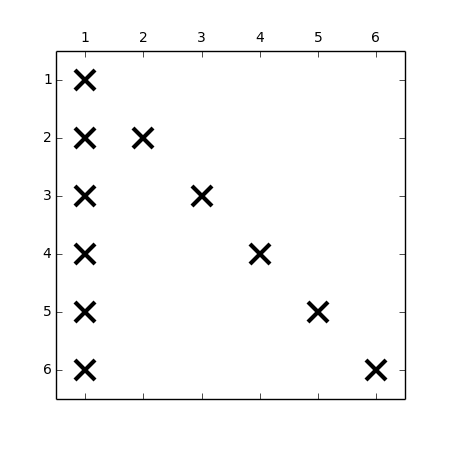
\includegraphics[width=0.3\linewidth]{diag-col}
\hfill
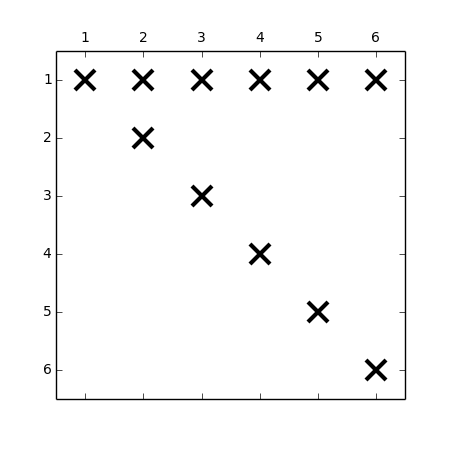
\includegraphics[width=0.3\linewidth]{diagrow}
\hfill
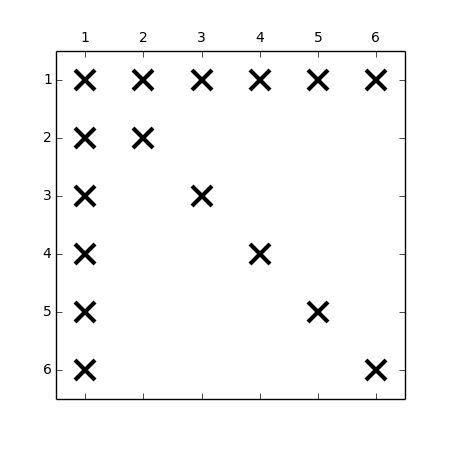
\includegraphics[width=0.3\linewidth]{arrow}
\caption{
(Left) An example of a matrix compressed efficiently by columns.
(Middle) An example of a matrix compressed efficiently by rows.
(Right) An example of a matrix which cannot be compressed efficiently either by columns nor by rows.
}
\label{f.mat-ex-for-orth}
\end{figure}
Now, consider the matrix in \figref{f.mat-ex-for-orth} (Right) that has neither structurally orthogonal columns nor structurally orthogonal rows.
Therefore, there is no unidirectional compression of the
matrix, neither by columns nor rows.
However, the technique of bidirectional compression, 
which compresses both columns and rows at the same time, 
will reduce the computational cost at that example. 
This technique uses both forward and reverse modes of automatic differentiation.

For general sparsity patterns,
it is not straightforward to figure out how to linearly combine columns and rows such that
the computational cost is minimized. Hence, we introduce the combinatorial
optimization problems~\ref{p.seed.uni} and ~\ref{p.seed.bid}
for unidirectional and bidirectional compression to determine 
the nonzero elements of large Jacobian matrices efficiently.

\begin{problem}[\MinUniCom]
\label{p.seed.uni} Let $J$ be a sparse ${m\times n}$ Jacobian matrix with a known sparsity
pattern. Find a binary seed matrix $V$ of dimension $n\times \col$
whose number of columns is minimized
such that all nonzero elements of $J$ also appear in
the matrix-matrix product $JV$.
\end{problem}

\begin{problem}[\MinBidCom]
\label{p.seed.bid} Let $J$ be a sparse ${m\times n}$ Jacobian matrix with known sparsity
pattern. Find a pair of binary seed matrices $V$ of dimension $n\times \col$ and $W$~of
dimension $\row \times m$ in which the number of columns of $V$ and the number of rows of $W$ sum up to a minimal value, $\col + \row$, such that all nonzero elements of $J$ also appear in
the pair of matrix-matrix products $JV$ and $WJ$.
\end{problem}

%==========================================================================================
\subsubsection{Combinatorial model}
\label{s.modeling.full}
%==========================================================================================
We reformulate the scientific computing problems which
we have discussed in \secref{ss.problem.full}.
The new formulation is an equivalent problem defined on a
carefully chosen graph model. The survey \cite{Gebremedhin05whatcolor}
discusses different methods
to exploit the sparsity involved in derivative computations.
We first look at a simple graph model for the unidirectional compression.
%
\begin{definition}[Column Intersection Graph]
\label{d:cig}
The column intersection graph $G = (V,E)$ associated with an $n \times n$ Jacobian matrix $J$
consists of a set of vertices $V=\{v_1, v_2, \dots, v_n\}$ whose vertex $v_i$ represents
the $i$th column $J(:,i)$. Furthermore, there is an edge $(v_i,v_j)$ in the set of edges
$E$ if and only if the columns $J(:,i)$ and $J(:,j)$ represented by $v_i$ and $v_j$ 
are structurally non-orthogonal.
\end{definition}

As we have a graph model interpreted from our Jacobian matrix in \defref{d:cig},
the grouping of columns can be encoded in the following well-known graph coloring problem.
%
\begin{definition}[Coloring]
A coloring of $G$ is a mapping $\Phi : V \to {1, \dots, p}$ with the property
$\Phi(v_i)\neq \Phi(v_j)$ if $(v_i,v_j) \in E$.
\end{definition}
%
Coleman and Mor\'{e} \cite{Coleman1983EoS} then showed that Problem~\ref{p.seed.uni}, which
asks for a seed matrix with a minimal number of columns, is equivalent to the following
coloring problem.

\begin{problem}[Minimum Coloring]
\label{p:mincol}
Find a coloring $\Phi$ of the column intersection graph $G$ with a minimal number of
colors.
\end{problem}

Although, this model is convincing for the unidirectional compression,
the bidirectional compression can not be an instance of this model.
A bidirectional compression needs the information of both rows and columns. Therefore, a bipartite graph model is defined for this purpose as in~\cite{Coleman1996SaE,cv:ecs,hs:csj}.

\begin{definition}[Bipartite Graph Model]
\label{d.bip.graph}
In the bipartite graph model, the vertex set $V=V_c\cup V_r$
is decomposed into a set of vertices~$V_c$ representing columns of $J$ and another set of
vertices~$V_r$ representing rows. The set of edges~$E$ is used to represent the nonzero
elements and it is defined as follows. An edge $(c_i , r_j) \in E$ connects a column
vertex $c_i \in V_c$ and a row vertex $r_j \in V_r$ if there is a nonzero element in $J$
at the position represented by $c_i$ and $r_j$. The graph is bipartite indicating that
all edges connect vertices from one set~$V_c$ to the other set $V_r$. That is, there is
no edge connecting vertices within the set $V_c$ or within $V_r$. Moreover, two vertices
that are connected by a path of length two, are called \emph{distance-$2$ neighbors}.
\end{definition}

The coloring problem in the column-intersection graph \ref{p.seed.uni} can also be represented in
this bipartite graph model. This equivalent coloring is done only in the set of
column vertices. Also, \emph{distance-$2$ neighbors} should be considered instead of
edges.

The overall idea behind transforming Problem \ref{p.seed.bid}, \MinBidCom, into an equivalent
problem using the bipartite graph model is as follows. The grouping of the columns and
rows is expressed by representing each group by a color. Vertices that belong to the same
group of columns/rows are assigned the same color. Formally, this is represented by a
coloring of a bipartite graph. Such a coloring is mapping
$$
\Phi:V_c \cup V_r \to \{0,1,\dots ,p\}
$$
that assigns to each vertex a color represented by an integer. 
The coloring~$\Phi$ also involves a ``neutral'' color
representing this ``don't color'' situation. A vertex $v \in V_c \cup V_r$ that is not
used in the grouping of columns/rows is assigned the neutral color $\Phi(v)=0$. More
precisely, if $\Phi(v)=0$ for a column vertex $v$ then every nonzero represented by an
incident edge of $v$ is determined by a linear combination of rows. Similarly, a nonzero
entry represented by an edge that is incident to a neutrally-colored row vertex is
determined by a linear combination of columns.

To represent the process of finding seed matrices using the bipartite graph model, it is
necessary to consider the underlying properties, which are as follows:
\begin{enumerate}
\item The computational cost roughly consists of the number of groups of columns and
rows. Since the overall cost is the sum of the costs associated with the forward mode
and the reverse mode, the (non-neutral) colors for the forward mode and the
(non-neutral) colors for the reverse mode need to be different.

\item It may happen that some nonzero
elements may be computed twice, by the forward mode in $JV$ and by the reverse mode
in $WJ$. Therefore, an edge representing such a nonzero element connects two
vertices with two different non-neutral colors. In general, since the
\MinBidCom problem asks for computing \emph{all} nonzero elements, at least one vertex of
every edge has to be colored with a non-neutral color.

\item Suppose two columns are structurally non-orthogonal and have a nonzero element in a
same row. If this row is not handled by the reverse mode, these two columns need to
be in different column groups. The same argument holds for corresponding situations
with row groups.

\item Consider three nonzero elements in the matrix positions $(i,k)$, $(i,\ell)$, and
$(j,k)$. Suppose that the nonzero at $(i,k)$ is computed by the reverse mode
assigning some (non-neutral) color to the row vertex $r_i$. Then, if $(j,k)$ is
also computed via the reverse mode, a second (non-neutral) color is needed for
$r_j$. Now, if $(i,\ell)$ is already determined by the reverse mode for the row $i$ the
column vertex $c_\ell$ is assigned the neutral color. However, if $(i,\ell)$ is
computed by the forward mode, a third (non-neutral) color is needed for $c_\ell$. A
similar argument holds if $(i,k)$ is computed by the forward mode.
\end{enumerate}

Based on these considerations, the following definition captures these properties.

\begin{definition}[Star Bicoloring]\label{d.coloring}
Given a bipartite graph $G=(V_c\cup V_r, E)$, then a mapping $\Phi:V_c \cup V_r \to
\{0,1,\dots ,p\}$ is a star bicoloring of $G$ if the following conditions are satisfied:
\begin{enumerate}
\item Vertices in $V_c$ and $V_r$ receive disjoint colors, except for the neutral color~$0$. That
is, for every $c_i \in V_c$ and $r_j \in V_r$, either $\Phi(c_i) \neq \Phi(r_j)$ or
$\Phi(c_i)=\Phi(r_j)=0$.

\item At least one vertex of every edge receives a non-neutral color. That is, for every
$(c_i,r_j)\in E$, the conditions $\Phi(c_i)\neq 0$ or $\Phi(r_j)\neq 0$ hold.

\item For every path $(u,v,w)$ with $\Phi(v) = 0$, the condition $\Phi(u)\neq \Phi(w)$ is
satisfied.
\item Every path of length three with four vertices uses at least three colors
(possibly including the neutral color).
\end{enumerate}
\end{definition}

Using the bipartite graph model and the definition of a star bicoloring, the problem
\MinBidCom\ is equivalent to the following graph problem.

\begin{problem}[\MinStaBic]
\label{p.coloring} Given the bipartite graph $G=(V_r\cup V_c, E)$ associated with a sparse Jacobian
matrix~$J$, find a star bicoloring of $G$ with a minimal number of non-neutral colors.
\end{problem}

A unidirectional compression is a special case of a bidirectional compression. More precisely, a
unidirectional compression with respect to columns corresponds to a star bicoloring in which all
the vertices in $V_c$ are colored with a non-neutral color and all row vertices are colored with
the neutral color. This way, the coloring constraint of a star bicoloring reduces to coloring
distance-$2$ neighbors in the bipartite graph using different (non-neutral) colors. This distance-2
coloring in the bipartite graph model is then equivalent to a coloring in the undirected graph
model in which all neighbors are colored differently. Finally, a discussion of the computational
complexity of Problem~\ref{p.coloring} including recent new results is given in~\cite{jj:cjr}.

%To illustrate the tricky transformation from \MinBidCom\ to \MinStaBic, we design a new
%educational module explained in Section~\ref{s.bidirectional}.
%%%%%%%%%%%%%%%%%%%%%%%%%%%%%%%%%%%%%%%%%%%%%%%%%%%%%%%%%%%%%%%%%%%%%%%%%%%%%%%%%%%%%%%%%%%%%%%%%%%%%%%%%
\subsection{Partial Jacobian computation}
\label{s.part.jac}
%%%%%%%%%%%%%%%%%%%%%%%%%%%%%%%%%%%%%%%%%%%%%%%%%%%%%%%%%%%%%%%%%%%%%%%%%%%%%%%%%%%%%%%%%%%%%%%%%%%%%%%%%
Gebremedhin et al.~\cite{Gebremedhin05whatcolor} introduced the concept of partial Jacobian computation
in which only a subset of Jacobian, the so-called required elements,
are to be determined.
L{\"u}lfesmann~\cite{Lulfesmann2012Fap} studied this area in more details and
introduced some heuristics for partial computation.
%%%%%%%%%%%%%%%%%%%%%%%%%%%%%%%%%%%%%%%%%%%%%%%%%%%%%%%%%%%%%%%%%%%%%%%%%%%%%%%%%%%%%%%%%%%%%%%%%%%%%%%%%
\subsubsection{Scientific computing problem}
\label{ss.problem.part}
%%%%%%%%%%%%%%%%%%%%%%%%%%%%%%%%%%%%%%%%%%%%%%%%%%%%%%%%%%%%%%%%%%%%%%%%%%%%%%%%%%%%%%%%%%%%%%%%%%%%%%%%%
Let $R$ be the set representing required elements. 
The definition of
\emph{structurally orthogonality} is adapted for partial Jacobian computation as follows,
\begin{definition}[Partially Structurally Orthogonal]\label{d.part.str.orth}
Two columns $c_i$ and $c_j$ are partially structurally orthogonal with respect to $R$
if and only if they do not have a nonzero element in a same row where at least
one of these nonzero elements is required.
\end{definition}

The corresponding combinatorial optimization problem for the unidirectional and bidirectional 
compression restricted to the required elements
can be formulated as follows.
\begin{problem}[\MinRUniCom]
\label{p.seed.runi} Let $J$ be a sparse ${m\times n}$ Jacobian matrix with known sparsity
pattern and $R$ be a subset of $J$. Find a seed matrix $V$ of dimension $n\times \col$
whose number of columns of $V$ sums up
to a minimal value, $\col$, such that all nonzero elements of $R$ also appear in
the matrix-matrix product $JV$.
\end{problem}

\begin{problem}[\MinRBidCom]
\label{p.seed.rbid} Let $J$ be a sparse ${m\times n}$ Jacobian matrix with known sparsity
pattern and $R$ be a subset of $J$.
Find a pair of binary seed matrices $V$ of dimension $n\times \col$ and $W$~of
dimension $\row \times m$ whose number of columns of $V$ and number of rows of $W$ sum up
to a minimal value, $\col + \row$, such that all nonzero elements of $R$ also appear in
the pair of matrix-matrix products $JV$ and $WJ$.
\end{problem}

Now, we discuss an equivalent graph-theoretical formulation of this problem.

\subsubsection{Combinatorial model}
Based on \cite{Gebremedhin05whatcolor,Lulfesmann2012Fap}, the definitions
of full Jacobian coloring are adapted for the restricted colorings as follows,
\begin{definition}[Restricted distance-$2$ coloring]\label{d.coloring.d2}
Given a bipartite graph $G=(V_c\cup V_r, E)$ and a subset of required edges
$E_R\subseteq E$, then a mapping $\Phi:V_c \to
\{0,1,\dots ,p\}$ is a distance-$2$ coloring
of $G$ restricted to $E_R$ if no column vertex gets a zero color and
for every path $(c_k,r_i,c_j)$ with $c_k, c_j\in V_c$, $r_i\in V_r$, and $(r_i,c_j)\in E_R$,
$\Phi(c_k) \neq \Phi(c_j)$.
\end{definition}
\begin{definition}[Restricted star bicoloring]\label{d.coloring.bicol}
Given a bipartite graph $G=(V_c\cup V_r, E)$ and a subset of required edges
$E_R\subseteq E$, then a mapping $\Phi:V_c \cup V_r \to
\{0,1,\dots ,p\}$ is a star bicoloring of $G$ restricted to $E_R$
if the following conditions are satisfied:
\begin{enumerate}
\item Vertices in $V_c$ and $V_r$ receive disjoint colors, except for the neutral color~$0$. That
is, for every $c_i \in V_c$ and $r_j \in V_r$, either $\Phi(c_i) \neq \Phi(r_j)$ or
$\Phi(c_i)=\Phi(r_j)=0$.

\item At least one end point of an edge in $E_R$ receives a nonzero color.
\item For every edge $(r_i,c_j)\in E_R$, $r_i, r_l\in V_r$, and
$c_j, c_k\in V_c$,
\begin{itemize}
\item if $\Phi (r_i) = 0$, then for every path $(c_k,r_i,c_j)$, $\Phi (c_k)\neq \Phi (c_j)$
\item if $\Phi (c_j) = 0$, then for every path $(r_i,c_j,r_l)$, $\Phi (r_i)\neq \Phi (r_l)$
\item if $\Phi (r_i) \neq 0$ and $\Phi (c_j) \neq 0$, then for every path $(c_k,r_i,c_j,r_l)$,
$\Phi (c_k)\neq \Phi (c_j)$ or $\Phi (r_i)\neq \Phi (r_l)$
\end{itemize}
\end{enumerate}
\end{definition}

Now, the optimization problems are formulated as follow.

\begin{problem}[Minimum Restricted Distance-$2$ Coloring]
\label{p.restricted.d2} Given the bipartite graph $G=(V_r\cup V_c, E)$
associated with a sparse Jacobian
matrix~$J$ and a set of required edges $E_R$,
find a distance-$2$ coloring of $G$ restricted to $E_R$
with a minimal number of non-neutral colors.
\end{problem}

\begin{problem}[Minimum Restricted Star Bicoloring]
\label{p.restricted.star} Given the bipartite graph $G=(V_r\cup V_c, E)$
associated with a sparse Jacobian
matrix~$J$ and a set of required edges $E_R$,
find a star bicoloring of $G$ restricted to $E_R$
with a minimal number of non-neutral colors.
\end{problem}


%%%%%%%%%%%%%%%%%%%%%%%%%%%%%%%%%%%%%%%%%%%%%%%%%%%%%%%%%%%%%%%%%%%%%%%%%%%%%%%%%%%%%%%%%%%%%
\section{Combining partial Jacobian computation and ILU}
\label{s.precond}
%%%%%%%%%%%%%%%%%%%%%%%%%%%%%%%%%%%%%%%%%%%%%%%%%%%%%%%%%%%%%%%%%%%%%%%%%%%%%%%%%%%%%%%%%%%%%
Given a large sparse nonsingular $n\times n$ Jacobian matrix $J$,
we are considering the solution to the following system of linear equations,
$$
J x = b,
$$
in which $x$ and $b$ are $n\times 1$ vectors. 
Iterative solvers are considered to be among the effective solution techniques~\cite{ilu2003}.
These solvers are matrix-free which makes AD as a suitable method of differentiation.

Iterative techniques are typically used with some set of
the preconditioning techniques~\cite{precond1,ilu2003}.
Rather than solving the previous system,
we can solve the preconditioned system
\begin{equation}
\label{e:precond}
M^{-1} J x= M^{-1} b,
\end{equation}
where the $n \times n$ matrix $M$ serves as a preconditioner that approximates
the coefficient matrix,
$$M \approx J.$$

It is well known \cite{ros:gra} that the reordering has an effect on the number and positions of
the fill-in elements. We are interested in a particular permutation matrix $P$ such that
reordering the Jacobian matrix with $P$ is of the following form,
$$
P^T J P =
\begin{bmatrix}
A_1 & 0   & \cdots & 0 & B_1^T \\
0   & A_2 & \cdots & 0  & B_2^T \\
\vdots& \vdots & \ddots & 0 & \vdots \\
0   &   0 & \cdots & A_p & B_p^T \\
B_1 & B_2 & \cdots & B_p& C
\end{bmatrix} .
$$
This approach, the so-called nested dissection ordering, is first 
introduced George~\cite{nested_diss1}. An extensive discussion 
can be found in \cite{ilu_ordering4}.

%%%%%%%%%%%%%%%%%%%%%%%%%%%%%%%%%%%%%%%%%%%%%%%%%%%%%%%%%%%%%%%%%%%%%%%%%%%%%%%%%%%%%%%%%%%%%
\subsection{Scientific computing problem}
\label{ss.problem.precond}
%%%%%%%%%%%%%%%%%%%%%%%%%%%%%%%%%%%%%%%%%%%%%%%%%%%%%%%%%%%%%%%%%%%%%%%%%%%%%%%%%%%%%%%%%%%%%
Today, there is no general and established
strategy on how to combine automatic differentiation with preconditioning. The reason is
that standard preconditioning techniques typically need access to individual nonzero
elements of the coefficient matrix whereas automatic differentiation gives efficient
access to a different level of granularity, namely rows or columns.
%In \cite{Lulfesmann2012Fap}, a novel strategy is explained.
%We discuss this method briefly here.

Common approaches to constructing the preconditioner $M$ are based on accessing individual
nonzero entries $J(i,j)$ of the Jacobian. For instance, diagonal scaling consists of the
diagonal matrix $M$ whose diagonal entries $M(i,i)$ are equal to $J(i,i)$ for all
$i=1,2,\dots, n$. Another option is to compute a decomposition of the form
$$M = LU$$
where $L$ is a unit lower triangular matrix and $U$ is an upper triangular matrix
resulting from performing Gaussian elimination on $J$ and dropping out nonzero elements
that would be generated by this process in certain predetermined positions. Similar to
diagonal scaling, this incomplete LU factorization (ILU) needs access to individual
nonzero entries of $J$ or segments of rows/columns of $J$. In general, accessing an
individual nonzero entry via automatic differentiation is as efficient as accessing a
complete column or row. In practice, an access to some individual nonzero entry is
therefore prohibitively expensive regarding computing time.
%\begin{figure}%
%\centering
%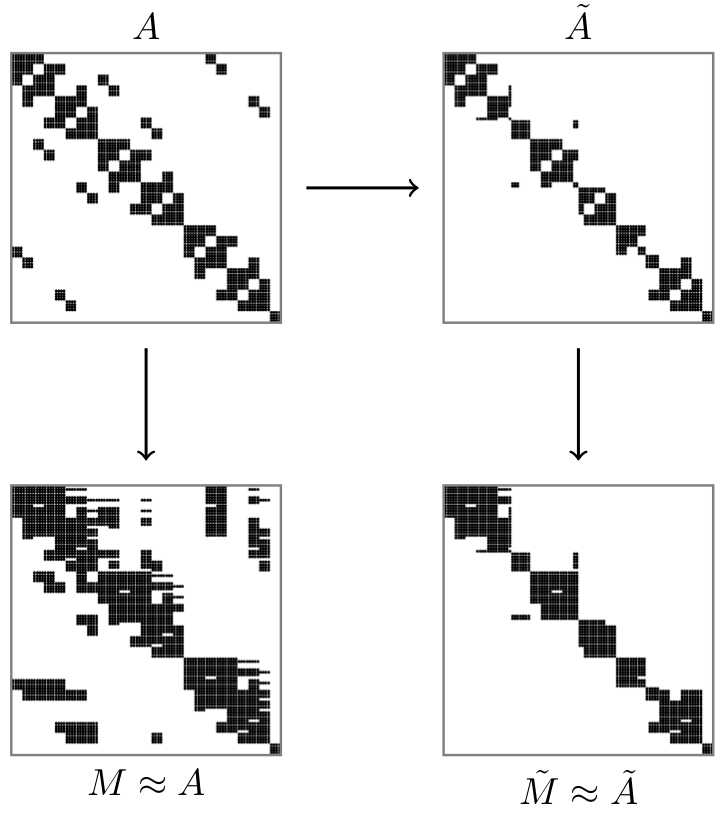
\includegraphics[width=0.5\linewidth]{combine_ad_ilu2.png}
%\caption{Determine the preconditioner~$M$ with access to all nonzero elements of Jacobian matrix~$A$. New approach: Determine the preconditioner~$\tilde M$ with access to a subset of $A$ using the sparsification operator~$\rho$. Based on Figure 4.1 from Lülfesmann~\cite{Lulfesmann2012Fap}.}%
%\label{f:luelfesmann-sparsify}%
%\end{figure}

Lülfesmann~\cite{Lulfesmann2012Fap} introduce new approach in which the required elements in matrix
are in the form of $k\times k$ blocks on the main diagonal.
Then, the preconditioner is built based on these selected nonzero required elements instead of
the whole Jacobian matrix.
Building a preconditioner based on a subset of the nonzero elements are explained in~\cite{Cullum2006}.
We call these required elements \textit{initially} required elements 
represented by $R_i$
since they are an initial set for the further process.
Now, the coloring problems~\ref{p.restricted.d2} 
and~\ref{p.restricted.star} can be solved for Jacobian
restricted to the set of initially required nonzero elements $R_i$. 

The result of a coloring algorithm groups columns and rows together.
In this processes, the required elements are always computed.
The remaining elements, the so-called nonrequired elements, 
are divided into two sets of
elements: the elements which are computed and the ones which would be
eliminated. We can think of these computed nonrequired nonzero elements as byproducts
of the coloring and computing the matrix-matrix products $JV$ and $WJ$.
Since the number of colors does not change,
the idea is to add these extra byproducts also to $R_i$.
However, it could generate new fill-ins in the preconditioning step.
So, we call these byproduct elements the \textit{potentially}
required elements $R_p$ and compute them as follows,
$$
R_p \subset \operatorname{pat}(J) - R_i \quad\text{so that}\quad |\Phi(R_i)| = |\Phi(R_i\cup R_p)|,
$$
while $\operatorname{pat}(J)$ represents the nonzero pattern of the Jacobian matrix $J$.

As we have discussed, an ILU preconditioner is applied to $R_i$ which can
produce a set of fill-ins.
Different methods can be employed to compute the preconditioner.
The overall approach applied to a specific problem from aerodynamic is detailed
in ~\cite{cscpaper}.

Now, a subset $R_a$ of potentially required elements, 
the so called \textit{additionally} required elements,
is selected such that no new fill-ins are generated which is called
additionally required elements $R_a$. These elements can be added to the
initially required elements for further computation.
The additionally required elements are formulated as follows,
$$
R_a \subset R_p \quad\text{so that}\quad SILU(R_i) \cup R_a = SILU(R_i\cup R_a),
$$
in which $SILU$ means the symbolic ILU factorization.

Now, we formulate two optimization problems in this thesis as follows,
\begin{problem}[Maximum Potentially Required Elements]
\label{p:max_pot}
%
Let $J$ be a sparse $m\times n$ Jacobian matrix with known sparsity pattern and
$R_i$ is a set of required elements.
Find a set of potentially required elements $R_p$ with maximal cardinality.
\end{problem}

\begin{problem}[Maximum Additionally Required Elements]
\label{p:max_add}
%
Let $J$ be a sparse $m\times n$ Jacobian matrix with known sparsity pattern and
$R_i$ is a set of required elements.
Find a set of additionally required elements $R_a$ with maximal cardinality.
\end{problem}

\subsection{Combinatorial model}
\label{ss.comb.precond}
The bipartite graph model presented in~\defref{d.bip.graph} is
a suitable model to find new algorithms for the initially, potentially,
and additionally required elements. 
Recall each edge in the bipartite graph model is related to a nonzero element in 
the matrix.
Then, given a bipartite matrix $G = (V,E)$,
three subsets $E_i, E_p, E_a\subset E$
are considered for the initially, potentially,
and additionally required elements, respectively.
Given the $k\times k$ block on diagonal as required elements $R_i$ and the Jacobian matrix $J$,
here is a list of steps in the computation of additionally required elements
and the corresponding algorithm on the bipartite graph model
(details in~\cite{Lulfesmann2012Fap}),
\begin{itemize}
\item compute the initially required elements $R_i$.
\item setup the bipartite graph $G$ from the Jacobian matrix $J$ and the subset $E_i\subset E$ representing $R_i$.
\item compute the coloring $\Phi_{G}(E_i)$ of the bipartite graph $G$ restricted to $E_i$.
\item find the set of potentially required elements $E_p\subset E - E_i$ such that $|\Phi_{G}(E_i)| = |\Phi_{G}(E_i \cup E_p)|$.
\item find the set of additionally required elements $E_a\subset E_p$ such
that $SILUR(R_i) \cup R_a = SILU(R_i \cup R_a)$. 
\end{itemize}
\coderef{code.pot.d2} and \coderef{code.pot.sb} show the algorithms to compute the
potentially required elements for the distance-$2$ coloring and star bicoloring, respectively.
In these algorithms, $N_1$ means the distance-$1$ neighbors (edges) and 
distance-$2$ neighbors.
Given a bipartite graph $G$, the required edges $E_i$, and a distance-$2$ coloring $\Phi$,
\coderef{code.pot.d2} computes a set of potentially required elements. This algorithm
iterates over nonrequired edges ($E - E_i$) and checks if such an edge can be added to the 
potentially required elements. Similarly, \coderef{code.pot.sb} computes 
the potentially required elements when the given coloring $\phi$ is star bicoloring.
\begin{figure}
\begin{lstlisting}[caption=Find potentially required elements for
distance-$2$ coloring,label=code.pot.d2,mathescape]
function pot_d2_coloring($G=(V_r\cup V_c,E)$,$E_i\subseteq E$,$\phi$)
  $E_p=\emptyset$
  for $(r_i,c_j)\in E-E_i$ with $\Phi(c_j)\neq 0$
    for $c_k\in N_1(r_i,G)$ with $j\neq k$ and $(r_i,c_k)\notin E_i$
      if $\Phi(c_j) = \Phi(c_k)$
        continue with next edge $(r_i,c_j)\in E-E_i$
    $E_p = E_p \cup {(r_i,c_j)}$
  return $E_p$
\end{lstlisting}
\end{figure}
\begin{figure}
\begin{lstlisting}[caption=Find potentially required elements for star bicoloring,label=code.pot.sb,mathescape]
function pot_star_bicoloring($G=(V_r\cup V_c,E)$,$E_i\subseteq E$,$\phi$)
  $E_p = \emptyset$
  for $(r_i,c_j)\in E-E_i$ with $\Phi(r_i)\neq 0$ or $\Phi(c_j)\neq 0$
    if $\Phi(r_i) = 0$
      for $c_k\in N_1(r_i,G)$ with $j\neq k$ and $(r_i,c_k)\notin E_i$
        if $\Phi(c_j)==\Phi(c_k)$
          continue with the next edge $(r_i,c_j)\in E - E_i$

    if $\Phi(c_j) = 0$
      for $r_l\in N_1(c_j,G)$ with $j\neq l$ and $(r_l,c_j)\notin E_i$
        if $\Phi(r_i)==\Phi(r_l)$
          continue with the next edge $(r_i,c_j)\in E - E_i$

    if $\Phi(r_i) \neq 0$ and $\Phi(c_j) \neq 0$
      for $c_k\in N_1(r_i,G)$ with $i\neq k$
        for $r_l\in N_1(c_j,G)$ with $j\neq l$
          if $\Phi(c_j)==\Phi(c_k)$ and $\Phi(r_i)==\Phi(r_l)$
            continue with the next edge $(r_i,c_j)\in E - E_i$

    $E_p = E_p \cup {(r_i,c_j)}$
  return $E_p$
\end{lstlisting}
\end{figure}

To compute the additionally required elements, a formulation of ILU preconditioning
in the language of graphs is needed.
Hysom and Pothen~\cite{precond-pothen} introduced a graph model for the incomplete
LU factorization in which the matrix is the adjacency matrix of this graph.
It should be considered that the graph would be directed if the matrix is not symmetric.
A concept of \textit{fill path} is defined to characterize the fill-ins in preconditioning,
\begin{definition}[Fill path]\label{d.fill.path}
A fill path is a path $(v_i,...,v_k,...,v_j)$ with
$k<min(i,j)$. It means the index of the all inner nodes in a given ordering of vertices
should be smaller than indices of the vertices $v_i$ and $v_j$.
\end{definition}
It follows that a matrix element $(i,j)$ is a fill-in if and only if there is a fill path between
$v_i$ and $v_j$.
In addition to the concept of fill path, another concept of fill level $l$ is needed to
formulate the level-based incomplete LU factorization~\cite{precond-pothen}.
This parameter is used to filter the generated fill-ins.
This parameter is the length of the fill path.
In the level-based incomplete LU factorization, the generated fill-ins are allowed
to be considered only up to the level $l$.
We fix this level parameter to $2$ throughout this thesis.

\begin{figure}
\begin{lstlisting}[caption=Find additionally required elements,
label=code.add,mathescape]
function add($G=(V_r\cup V_c,E)$,$E_i\subseteq E$,$E_p$)
  $E_a = \emptyset$
  do
    for $(r_i,c_j)\in E_p$
      if $i > j$
        for $c_l\in N_1(r_j,G[E_i\cup (E_F\cup E_a)])$ with $l > j$
          if $(r_i,c_j)\notin E_i\cup (E_F\cup E_a)$
            continue with next edge $(r_i,c_j)\in E_p$
      else if $i > j$
        for $r_k\in N_1(c_i,G[E_i\cup (E_F\cup E_a)])$ with $k > i$
          if $(r_k,c_j)\notin E_i\cup (E_F\cup E_a)$
            continue with next edge $(r_i,c_j)\in E_p$
      $E_a = E_a \cup {(r_i,c_j)}$
      $E_p = E_p - {(r_i,c_j)}$
  while $|E_a|$ is increased in the last iteration
  return $E_a$
\end{lstlisting}
\end{figure}
Lülfesmann~\cite{Lulfesmann2012Fap} adapted a
corresponding bipartite graph model for ILU preconditioning.
The concept of fill path is also redefined for the bipartite graph model
in which a path is replaced by a distance-$2$ path.
\begin{definition}[Fill path in bipartite graph]\label{d.fill.path.bipartite}
A path $(r_i,c_k,r_k,c_l,r_l,...,c_j)$ in the bipartite graph model starting
from a row vertex is an fill path 
if and only if all vertices between $r_i$ and $c_j$ have a lower index than $i$
and $j$. 
\end{definition}
Again, it follows that 
there is a fill-in $(i,j)$ in the matrix if and only if there is a
fill path between $r_i$ and $c_j$ in the corresponding bipartite graph.

Based on the bipartite graph models for coloring and the ILU preconditioning,
two algorithms are proposed to compute the additionally required
elements: conservative and sophisticated. 
We consider the sophisticated algorithm shown in \coderef{code.add}
to compute the additionally required elements
throughout this thesis. This algorithm looks at each potentially required edge.
If it is possible that a fill path generated by adding this edge,
the edge is not considered for the set of additionally required edges.
In this sophisticated approach, the algorithm iterates once again over 
all potentially required elements. This processes repeated until 
no new additionally required edges are found.

%%%%%%%%%%%%%%%%%%%%%%%%%%%%%%%%%%%%%%%%%%%%%%%%%%%%%%%%%%%%%%%%%%%%%%%%%%%%%%%%%%%%%%%%%%%%%%%%%%%%%%%%%%%%%%%%%%%%%%%%%%%%%%%%
%%%% PRECONDITIONING AND COLORING
%%%%%%%%%%%%%%%%%%%%%%%%%%%%%%%%%%%%%%%%%%%%%%%%%%%%%%%%%%%%%%%%%%%%%%%%%%%%%%%%%%%%%%%%%%%%%%%%%%%%%%%%%%%%%%%%%%%%%%%%%%%%%%%%
\chapter{New coloring heuristics}
\label{package}
Karp~\cite{karp:1972} proves that the graph coloring problem is NP-complete for general graphs.
Hence, various coloring heuristics are studied throughout the years with a polynomial complexity.
The greedy coloring is a widely used heuristic which has a low computational complexity
and computes a \textit{reasonable} coloring (see~\cite{spaa14}).
The greedy coloring algorithm for the restricted distance-$2$ coloring
is given in \coderef{code.greedy} which is adapted from Lülfesmann~\cite{Lulfesmann2012Fap}.
The computed coloring $\Phi:V_c\to\{1,2,...,p\}$ on the vertex set $V_c=\{1,2,...,n\}$
is restricted to the initially required edges $E_i$.
All arrays in all algorithms, like $forbiddenColors$, 
implemented in this thesis start with the index $0$.
The assignment $forbiddenColors[c]=v$ means the vertex $v$ can not be colored
by the color $c$. Since this algorithm does not consider the color $0$,
the element $forbiddenColors[0]$ is ignored.

In this algorithm, the function $N_2(v,E_i)$ finds all distance-$2$ neighbors
of $v$ restricted to the set of initially required edges $E_i$. 
More clearly, the function $N_2(v,E_i)$ computes 
all vertices on all paths of length $2$ from the vertex $v$
such that at least one edge of such a path is in the set $E_i$,
$$
N_2(v,E_i)=\{ z\in V: \text{ there is a path } (v,w,z) \text{ with } (v,w)\in E_i
\text{ or } (w,z)\in E_i \text{ or both.}\} 
$$
To color a vertex $v$ we iterate over all distance-$2$ neighbors in $N_2(v,E_i)$ which are
already colored. Remember that these assigned colors can not be used to color the vertex $v$.
After collecting all these forbidden colors, we assign $v$ color with a smallest index different from 
these forbidden colors.
It follows that the computational complexity of this algorithm is $\mathcal{O}(n \Delta^2)$ in which $n$
and $\Delta$ are the number of vertices and the maximum vertex degree, respectively.
Recall from the last chapter, the matrices are sparse. Therefore, $n$ is large and $\Delta$ and $\Delta^2$
are relatively small.

\begin{figure}
\begin{lstlisting}[caption=The greedy algorithm for
the distance-$2$ coloring restricted to the edge set $E_i$
for columns.,label=code.greedy,mathescape]
function d2_color($G=(V_r\cup V_c,E)$,$E_i\subseteq E$)
  $\Phi\leftarrow [0\ldots 0]$
  $forbiddenColors\leftarrow [0\ldots 0]$
  for $v\in V_c$ with $N_2(v,E_i)\neq\emptyset$
    for $n\in N_2(v,E_i)$ with $\Phi(n) \neq 0$
        $forbiddenColors[\Phi(n)] = v$
    $\Phi(v) = \min \{ a>0:forbiddenColors[a]\neq v\}$
  return $\Phi$
\end{lstlisting}
\end{figure}

In this algorithm, vertices are colored one at a time.
Therefore, the vertex ordering plays a major role in the greedy algorithm.
Hence, there are many publications on how to choose
a suitable ordering heuristics for a serial or parallel version of
coloring~\cite{ordering1,ordering2,ordering3}.
Various orderings are studied for coloring heuristics
throughout the years. Here are some orderings for coloring which are applied before doing the coloring:
the largest-first ordering (LFO)~\cite{LFO}, the incidence-degree ordering (IDO)~\cite{IDO},
the saturation-degree ordering (SDO)~\cite{SDO}, and the smallest-last ordering (SLO)~\cite{ordering1}.
A short description of these orderings is available in \appref{app.ord}.

This chapter is structured as follows.
We modify the greedy algorithm in \secref{s.max.pot.req} and \secref{s.max.add.req}
 such that the number of potentially required elements
and additionally required elements are increased.
Later, we discuss a better heuristic for
the special case of coloring restricted to a diagonal in~\secref{s.part.color.diag}.
We sketch the first ideas toward a new heuristic based on the exact coloring in small
subgraphs in~\secref{s.exact}.
Finally, we introduce our computational package \textit{PreCol} 
in~\secref{s.extend} that computes the 
unidirectional and bidirectional restricted colorings with different algorithms
as well as the ILU preconditioning. 

Throughout this chapter, the numerical experiments are carried out using 
the matrices in Table~\ref{florida.mats} from the Florida sparse matrix collection~\cite{florida.matrices}.
\begin{table}
\centering
\begin{tabular}{|c|c|c|c|}
\hline
Matrix & Size & Nonzeros & Symmetric\\\hline
\textit{steam1.mtx} & $240\times 240$ & $2248$ & false\\\hline
\textit{steam2.mtx} & $600\times 600$ & $5660$ & false\\\hline
\textit{685\_bus.mtx} & $685\times 685$ & $3249$ & true\\\hline
\textit{nos3.mtx} & $960\times 960$ & $15844$ & true\\\hline
\textit{ex7.mtx} & $1633\times 1633$ & $46626$ & false\\\hline
\textit{ex33.mtx} & $1733\times 1733$ & $22189$ & true\\\hline
\textit{orani678.mtx} & $2529\times 2529$ & $90158$ & false\\\hline
\textit{cavity16.mtx} & $4562\times 4562$ & $137887$ & false\\\hline
\textit{crystm01.mtx} & $4875\times 4875$ & $105339$ & true\\\hline
\textit{rajat01.mtx} & $6833\times 6833$ & $43250$ & false\\\hline
\textit{gyro\_m.mtx} & $17361\times 17361$ & $340431$ & true\\\hline
\textit{ford2.mtx} & $100196\times 100196$ & $544688$ & true\\\hline
\textit{cage3.mtx} & $5\times 5$ & $19$ & false\\\hline
\textit{cage4.mtx} & $9\times 9$ & $49$ & false\\\hline
\textit{cage5.mtx} & $37\times 37$ & $233$ & false\\\hline
\textit{cage6.mtx} & $93\times 93$ & $785$ & false\\\hline
\textit{cage7.mtx} & $340\times 340$ & $3084$ & false\\\hline
\textit{cage8.mtx} & $1015\times 1015$ & $11003$ & false\\\hline
\textit{cage9.mtx} & $3534\times 3534$ & $41594$ & false\\\hline
\textit{cage10.mtx} & $11397\times 11397$ & $150645$ & false\\\hline
\textit{cage12.mtx} & $130228\times 130228$ & $2032536$ & false\\\hline
\end{tabular}
\caption{
Throughout this chapter, the numerical experiments are carried out using 
these matrices from the Florida sparse matrix collection.}
\label{florida.mats}
\end{table}

%%%%%%%%%%%%%%%%%%%%%%%%%%%%%%%%%%%%%%%%%%%%%%%%%%%%%%%%%%%%%%%%%%%%%%%%%%%%%
\section{Maximizing the set of potentially required elements}
\label{s.max.pot.req}
%%%%%%%%%%%%%%%%%%%%%%%%%%%%%%%%%%%%%%%%%%%%%%%%%%%%%%%%%%%%%%%%%%%%%%%%%%%%%
Here, our focus is to solve Problem~\ref{p:max_pot}.
As we have discussed, there are nonrequired nonzero elements
which are also computed as a by-product of the computation of required elements.
The nonrequired elements have a major effect on
the determination of potentially required elements
and additionally required elements.
The following example illustrates that
a modified coloring can increase the number of nonrequired elements
which are determined.
\newcolumntype{r}{>{\columncolor{red!60}}c}
\newcolumntype{b}{>{\columncolor{blue!60}}c}
\begin{equation}
\left(\begin{array}{rrb}
* & * & *\\
0 & r & r \\
* & 0 & *
\end{array}\right)
\qquad
\left(\begin{array}{rbr}
* & * & *\\
0 & r & r \\
* & 0 & *
\end{array}\right)
\label{twocolorings}
\end{equation}
Here, the symbol $r$ stands for a required element,
the symbol \textit{$*$} stands for other nonzero elements (the nonrequired elements),
and the number $0$ denotes a zero element.
If the first and second columns get the same color as given in the left matrix,
we will get the nonzero at position $(3,1)$ as a by-product.
However, there are certain degrees of freedom. In
this example, one could also assign the same color to columns $1$ and
$3$ as illustrated in the right matrix
in which no nonzero element in the last row will be computed
as a by-product. This idea leads to the problem of maximizing
the number of nonrequired nonzero elements that are computed as a by-product.
Here, we introduce a new heuristic which increases the number of determined nonrequired elements 
while the number of colors remains almost the same.

\subsection{Restricted distance-$2$ coloring}
Our goal here is to increase the number of potentially required elements.
A potentially required element is selected from the nonrequired elements such that
the number of colors does not increase.
Given a bipartite graph $G=(V_c\cup V_r,E)$ and a vertex $v\in V_c$, 
we define a function $\nreq_v:S\subseteq V_c\rightarrow \mathbb{N}$.
The function $\nreq_v(w)$ computes the number of determined nonrequired elements
in the linear combination of the columns corresponding to the vertices $v$ and $w$.
We call these elements the determined nonrequired elements.
\begin{figure}
\begin{lstlisting}[caption=New coloring heuristic for distance-$2$ coloring
considering the nonrequired elements.,label=code.new.d2.nreq,mathescape]
function d2_color_nreq($G=(V_r\cup V_c,E)$,$E_i\subseteq E$)
  $\Phi\leftarrow [0\ldots 0]$
  $forbiddenColors\leftarrow [0\ldots 0]$
  for $v\in V_c$ with $N_2(v,E_i)\neq\emptyset$ and $\Phi(v)=0$
    for $n\in N_2(v,E_i)$ with $\Phi(n) \neq 0$
      $forbiddenColors[\Phi(n)] = v$
    $\Phi(v) = \min \{ a>0:forbiddenColors[a]\neq v\}$

    Determine an indepentent set $I_v$ containing $v$
    if $I_v-\{v\}\neq\emptyset$
      $maxs = \argmax_{x\in I_v - \{v\}} \nreq_v (x)$
      $\Phi(maxs[0]) = \Phi(v)$
  return $\Phi$
\end{lstlisting}
\end{figure}
Here, we focus on the unidirectional compression for columns represented by $V_c$.
However, an analogous discussion holds for the unidirectional compression for rows.

We modify the greedy algorithm  presented in \coderef{code.greedy} as follows.
Our approach in this new coloring algorithm is based on finding independent sets.
In a general graph $G=(V,E)$, a subset of the vertices $I\subseteq V$ is
called an independent set~\cite{bondy2008graph} 
if there is no edge between any of its vertices,
$$\forall u,v\in I: (u,v)\notin E.$$
In the bipartite graph model in \defref{d.bip.graph} with a set of initially required elements $E_i$,
we need to change the definition of an independent set using the distance-$2$ neighbors as follows,
$$\forall u,v\in I: u\notin N_2(v).$$
Also, we represent an independent set containing the vertex $v$ by $I_v$.
This set represents the vertices which can have same colors.
Here, we use this adapted definition for simplicity. 
Other definitions are possible using $N_2(v,E_i)$ which
may result in a more efficient heuristic.

For this new heuristic, we define two operators.
Given a function $f:A\rightarrow B$ and a subset $S\subseteq A$
the operators $\argmax$ and $\argmin$ are defined as,
\begin{equation*}
\begin{split}
\argmax_{x\in S} f(x) &= \{ x | \forall y\in S: f(y) \leq f(x)\}, \\
\argmin_{x\in S} f(x) &= \{ x | \forall y\in S: f(y) \geq f(x)\}.
\end{split}
\end{equation*}

\coderef{code.new.d2.nreq} shows this new heuristic.
In this algorithm, we iterate over all uncolored vertices.
First, we color the vertex $v$ with a color different form
its distance-$2$ neighbors restricted to $E_i$ like the previous greedy coloring.
Additionally, we compute $\nreq_v(x)$ for each vertex $x\in I_v$
and color a vertex $w\neq x$ with the same color as $v$ 
if $w$ leads to the maximum value of $\nreq_v(w)$
The time complexity of this new heuristic is estimated as follows.
We go through all vertices $v$
and find a maximum independent set $I_v$ containing $v$.
Then, we compute $maxs = \argmax_{x\in I_v - \{v\}} \nreq_v (x)$.
The computations of both sets $I_v$ and $maxs$ are of $\mathcal{O}(n^2)$.
That results in the computational complexity of $\mathcal{O}(n^3)$.

Although we color a vertex $v$ and another vertex $u\in I_v$ in each iteration
it does not always mean that the coloring is valid. Consider the following example.
\begin{equation}
\left(\begin{array}{cccc}
r & 0 & 0 & 0  \\
0 & 0 & r & 0 \\
0 & * & * & 0 \\
0 & r & 0 & r \\
\end{array}\right)
\label{twocolorings2}
\end{equation}
\coderef{code.new.d2.nreq} colors the first and second columns with the same color
in the first step. Then, the third column is colored with the same color as the
first column since there is no conflict. The fourth column gets the color of
the third column. However, this is not a valid coloring
since the fourth and second columns can not be compressed.
\begin{figure}
\begin{lstlisting}[
label=consistency,caption=A function validates the coloring.,mathescape]
function validate_coloring($G=(V_r\cup V_c,E)$,$E_i\subseteq E$)
  modified = false;
  do
    for $v \in V_c$ and $n \in N_2(v,E_i)$
      if $\Phi(n) == \Phi(v)$
        $\Phi(n) = $ a color different from its distance-$2$ neighbors
        modified = true
  while modified
  return $\Phi$
\end{lstlisting}
\end{figure}
Considering this problem, we validate the coloring at the end of the algorithm
by the function given in \coderef{consistency}.
In this function, we check if the color of each vertex $v$ is different than its distance $2$ neighbors restricted
 to $E_i$.
If not, the colors of that vertex change to some color different from its distance-$2$ neighbors.
This algorithm repeats this process until no new such vertex is found.

Table~\ref{mats.pot.add.gr.vs.nreq} presents the number of potentially
and additionally required elements computed
by \coderef{code.greedy} and \coderef{code.new.d2.nreq}
and for different orderings for coloring.
Table~\ref{mats.pot.add.gr.vs.nreq} (Top), (Middle), and (Bottom) are
the results for the natural ordering, the LFO ordering, and the SLO ordering, respectively.
The size of diagonal blocks is fixed to $10$.
In these tables, the numbers of both potentially required elements and additionally required elements 
are increased in the new proposed \coderef{code.new.d2.nreq} regardless of the ordering.
An observation is that although the number of potentially required elements decreases 
in the computation of the matrix $pesa.mtx$ with the ordering LFO,
the number of additionally required elements increases. However,
both the numbers of potentially and additionally required elements
are larger in the computation for \textit{ex7.mtx} and for all orderings.

\begin{table}
\centering
\begin{tabular}{|c|c|c|c|c|}
\hline
Matrix (NAT) & \multicolumn{2}{c|}{$|R_{pot}|$} & \multicolumn{2}{c|}{$|R_{add}|$}\\\hline
{} & \coderef{code.greedy} & \coderef{code.new.d2.nreq} & \coderef{code.greedy} & \coderef{code.new.d2.nreq}\\\hline
\textit{steam1.mtx} & $64$ & $786$ & $64$ & $630$ \\\hline
\textit{steam2.mtx} & $240$ & $1880$ & $240$ & $1400$ \\\hline
\textit{nos3.mtx} & $1638$ & $6756$ & $1106$ & $4296$ \\\hline
\textit{crystm01.mtx} & $17822$ & $47556$ & $10388$ & $28318$ \\\hline
\textit{ex7.mtx} & $38554$ & $34954$ & $29174$ & $25054$ \\\hline
\textit{ex33.mtx} & $7408$ & $8934$ & $4920$ & $5572$ \\\hline
\textit{coater1.mtx} & $11722$ & $11558$ & $7684$ & $7448$ \\\hline
\textit{pesa.mtx} & $36972$ & $41154$ & $31010$ & $33094$ \\\hline
\end{tabular}
\vspace*{1cm}\newline
\begin{tabular}{|c|c|c|c|c|}
\hline
Matrix (LFO) & \multicolumn{2}{c|}{$|R_{pot}|$} & \multicolumn{2}{c|}{$|R_{add}|$}\\\hline
{} & \coderef{code.greedy} & \coderef{code.new.d2.nreq} & \coderef{code.greedy} & \coderef{code.new.d2.nreq}\\\hline
\textit{steam1.mtx} & $64$ & $1048$ & $64$ & $666$ \\\hline
\textit{steam2.mtx} & $240$ & $2624$ & $240$ & $1248$ \\\hline
\textit{nos3.mtx} & $1880$ & $6882$ & $1246$ & $4442$ \\\hline
\textit{crystm01.mtx} & $20326$ & $36634$ & $12256$ & $21194$ \\\hline
\textit{ex7.mtx} & $37080$ & $33426$ & $28904$ & $24060$ \\\hline
\textit{ex33.mtx} & $10574$ & $10564$ & $7170$ & $6888$ \\\hline
\textit{coater1.mtx} & $11312$ & $11512$ & $7410$ & $7536$ \\\hline
\textit{pesa.mtx} & $42490$ & $41676$ & $31790$ & $31884$ \\\hline
\end{tabular}
\vspace*{1cm}\newline
\begin{tabular}{|c|c|c|c|c|}
\hline
Matrix (SLO) & \multicolumn{2}{c|}{$|R_{pot}|$} & \multicolumn{2}{c|}{$|R_{add}|$}\\\hline
{} & \coderef{code.greedy} & \coderef{code.new.d2.nreq} & \coderef{code.greedy} & \coderef{code.new.d2.nreq}\\\hline
\textit{steam1.mtx} & $64$ & $1294$ & $64$ & $754$ \\\hline
\textit{steam2.mtx} & $240$ & $3192$ & $240$ & $1912$ \\\hline
\textit{nos3.mtx} & $1682$ & $6772$ & $1132$ & $4382$ \\\hline
\textit{crystm01.mtx} & $24478$ & $45166$ & $14252$ & $26782$ \\\hline
\textit{ex7.mtx} & $36486$ & $34448$ & $27044$ & $24164$ \\\hline
\textit{ex33.mtx} & $8024$ & $10754$ & $5186$ & $7138$ \\\hline
\textit{coater1.mtx} & $10476$ & $11702$ & $7004$ & $7878$ \\\hline
\textit{pesa.mtx} & $39606$ & $44624$ & $29034$ & $34044$ \\\hline
\end{tabular}
\caption{The comparison between the number of potentially and additionally required
elements computed with \coderef{code.new.d2.nreq} and \coderef{code.greedy}.
The block size is fixed to $10$. The orderings for coloring are (Top) the natural ordering,
(Middle) LFO, and (Bottom) SLO.}
\label{mats.pot.add.gr.vs.nreq}
\end{table}


Now, we compare the results by changing the block size varying from $1$ to $70$.
We compute \coderef{code.greedy} and \coderef{code.new.d2.nreq} for the matrices \textit{ex33}
and \textit{crystm01} with the three different orderings: the natural ordering, the LFO ordering,
and the SLO ordering. Additionally, we compute the number of colors in each case too.
All figures are illustrated in \appref{app.compare.alg31.alg32}.
An observation is that the behavior of the figures of the potentially required elements and
the additionally required elements is the same. Hence, we consider only the additionally
required elements now.
The number of additionally required elements computed by \coderef{code.new.d2.nreq} with the ordering SLO
is overall larger than \coderef{code.greedy} (see \figref{ex33_alg31_alg32_bls_slo_add}).
The number of colors remains almost the same for the both colorings 
(see \figref{ex33_alg31_alg32_bls_slo_cols}). 
In the other orderings, this happens only in the middle block sizes, like from 25 to 60.
For example, \figref{ex33_alg31_alg32_bls_nat_add} shows the number of additionally required elements
compared when the natural ordering is considered.
However, the number of colors in this ordering is even more similar in both algorithms
(see \figref{ex33_alg31_alg32_bls_nat_cols}).
%The number of colors in~\figref{bls_cols_ex33_without_alpha} for the greedy coloring
%is the minimum value between different orderings \textit{LFO}, \textit{SLO}, and \textit{IDO}.

\begin{figure}
\centering
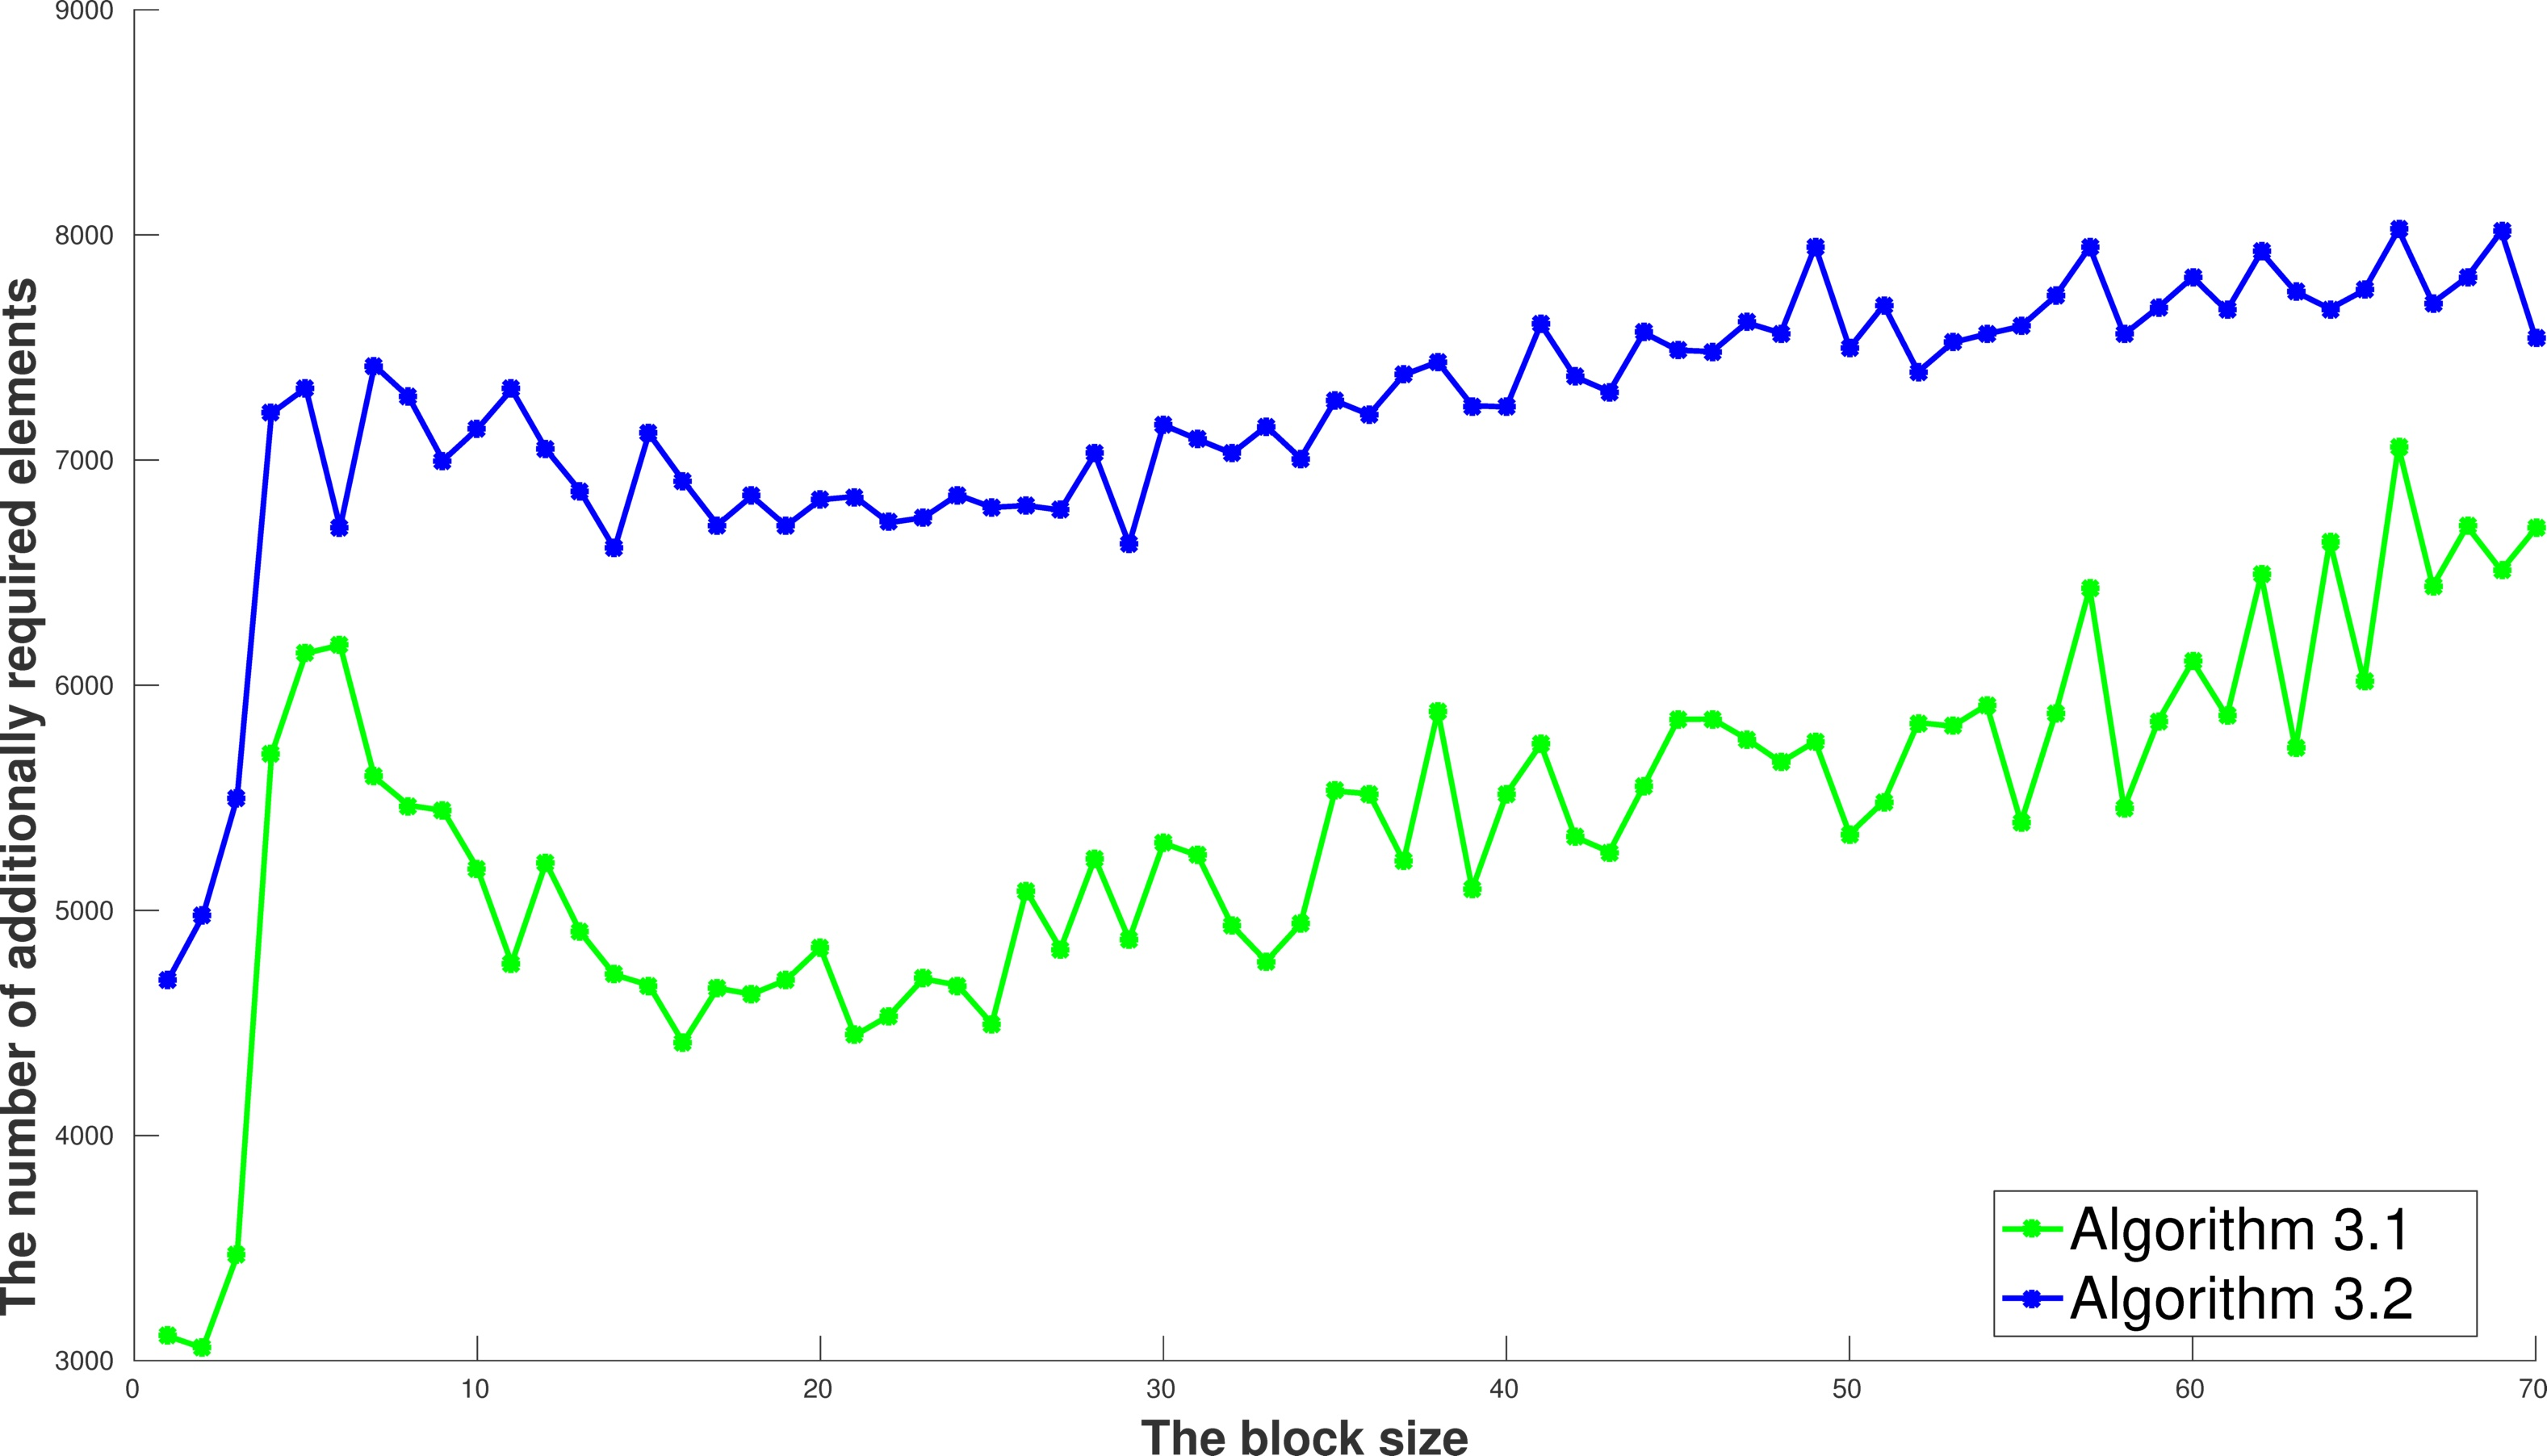
\includegraphics[width=0.9\linewidth]{ex33_alg31_alg32_bls_slo_add}
\caption{
The number of additionally required elements computed by
\coderef{code.new.d2.nreq} with the SLO ordering
compared with \coderef{code.greedy}.
The computation is carried out on the matrix \textit{ex33}. }
\label{ex33_alg31_alg32_bls_slo_add}
\end{figure}

\begin{figure}
\centering
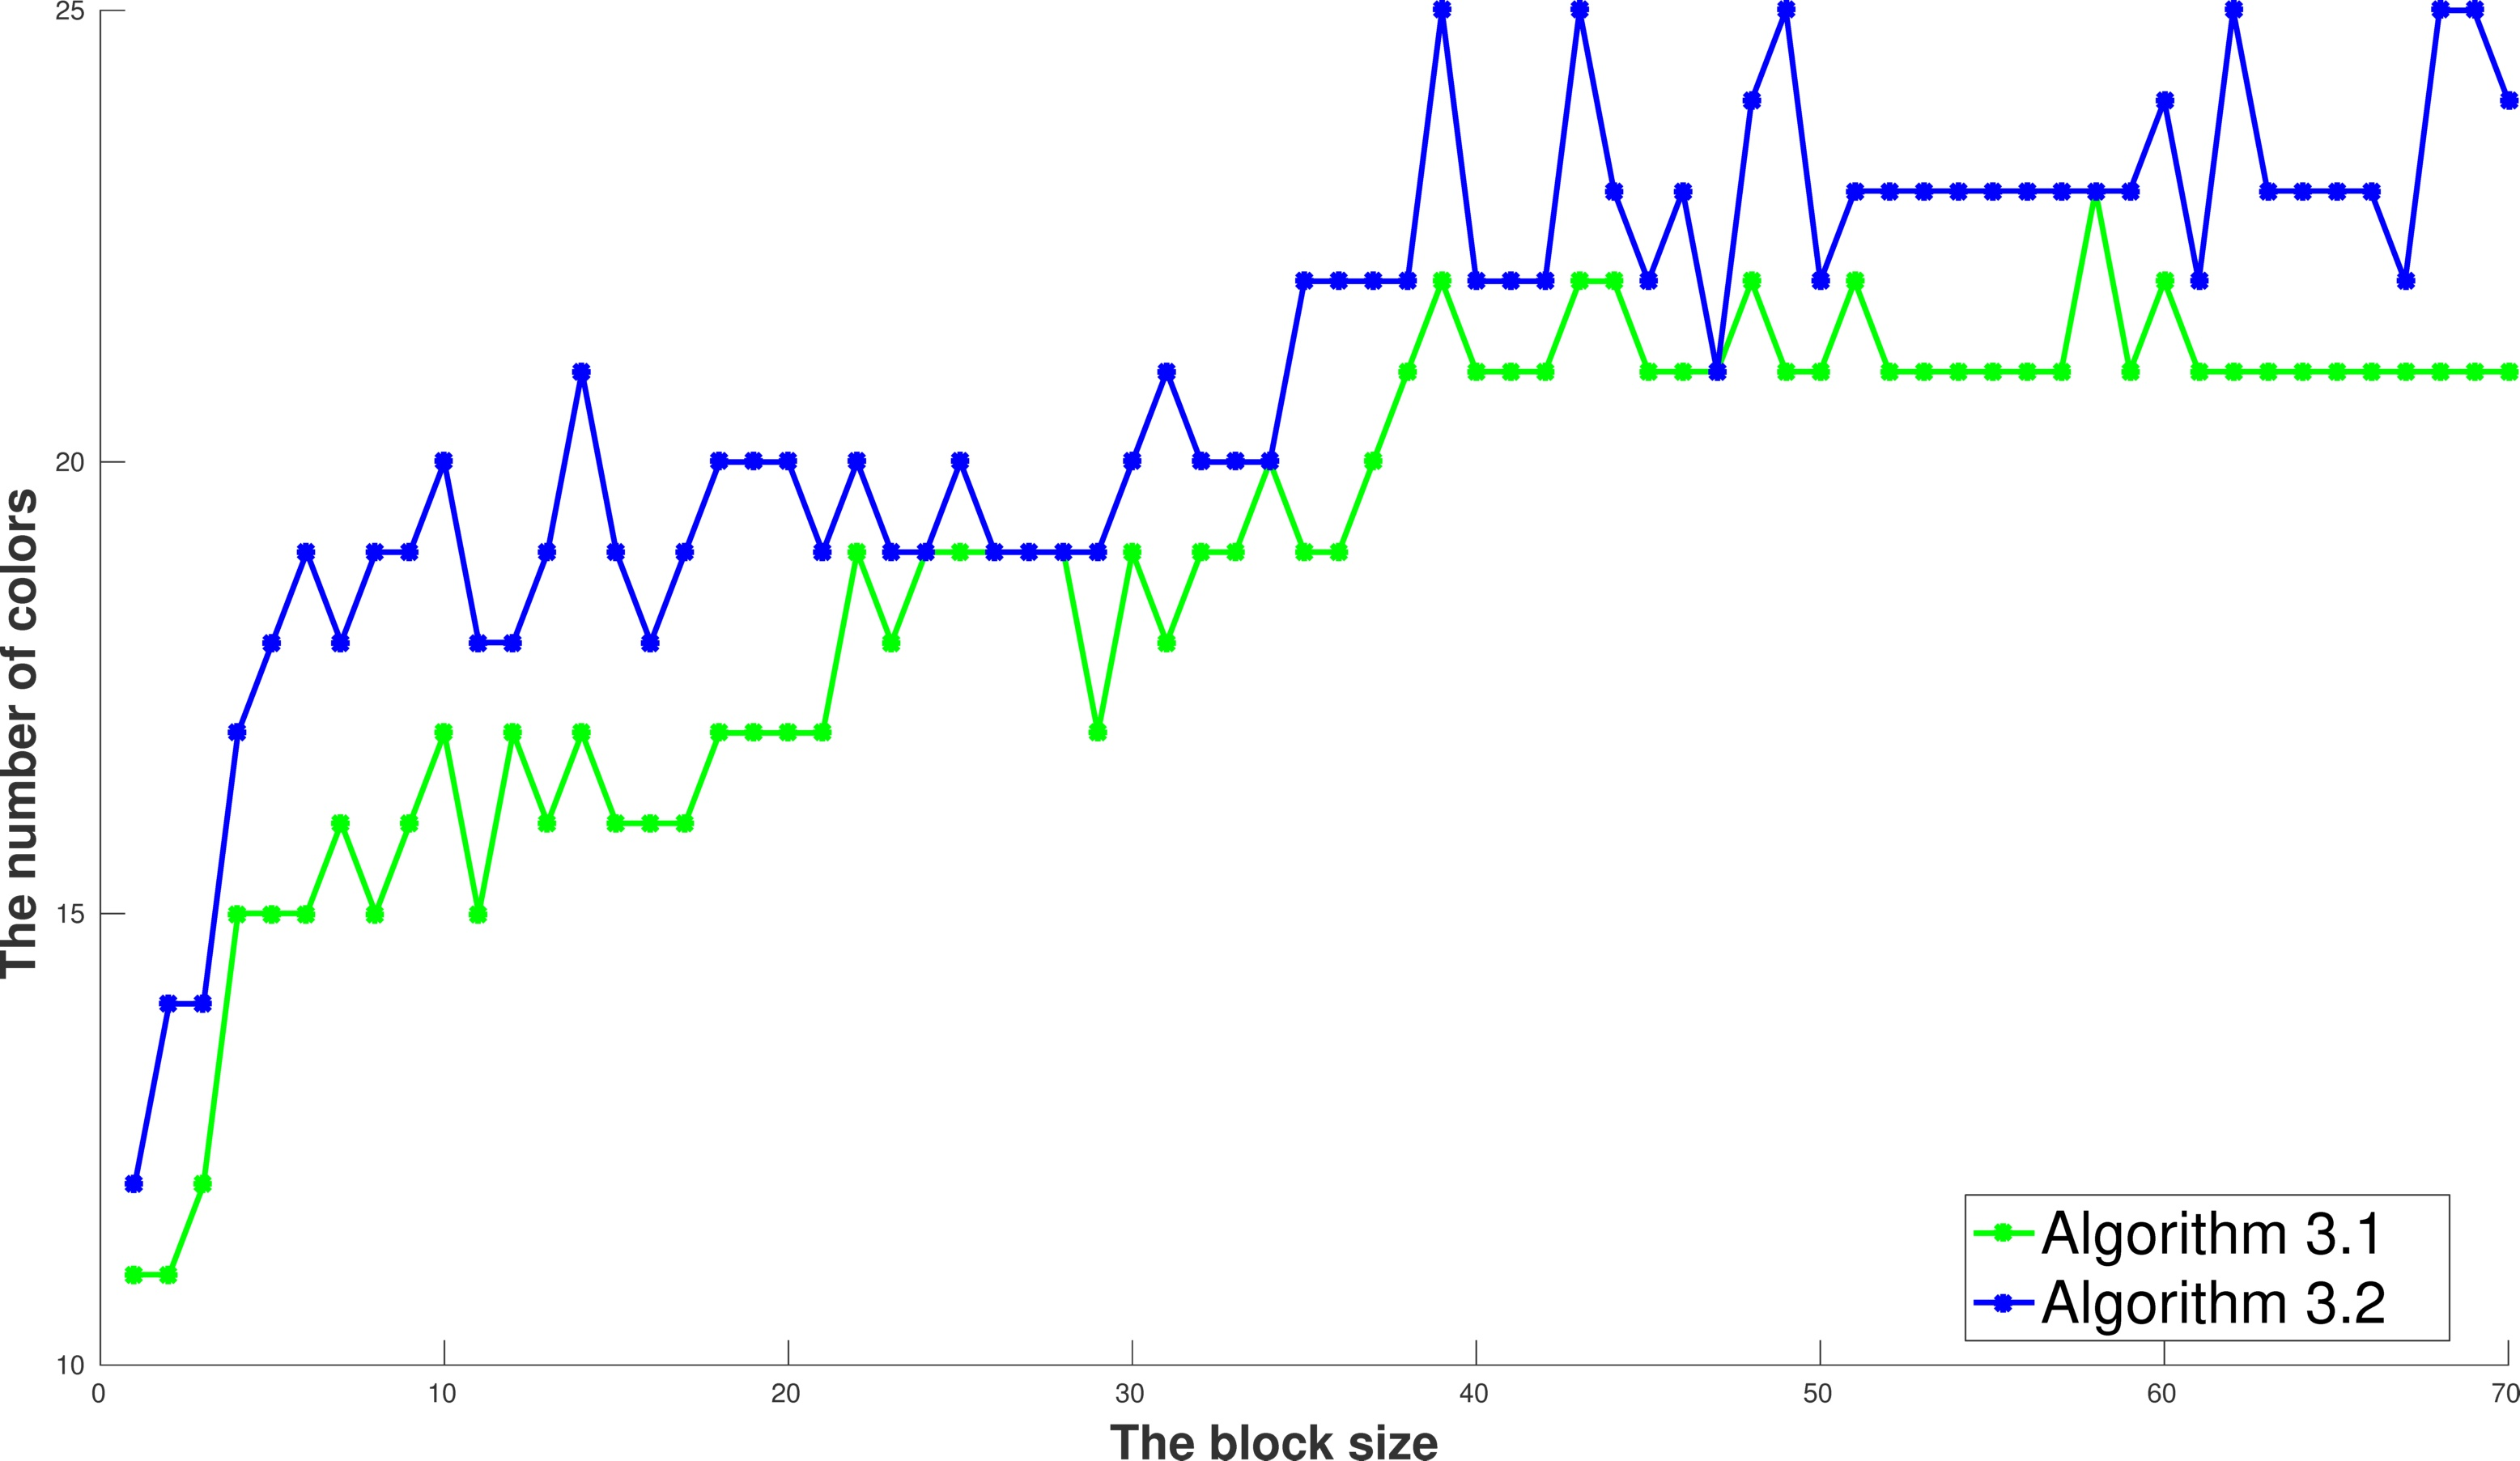
\includegraphics[width=0.9\linewidth]{ex33_alg31_alg32_bls_slo_cols}
\caption{The number of colors computed by \coderef{code.new.d2.nreq} with the SLO ordering
compared with \coderef{code.greedy}. 
The computation is carried out on the matrix \textit{ex33}.}
\label{ex33_alg31_alg32_bls_slo_cols}
\end{figure}

\begin{figure}
\centering
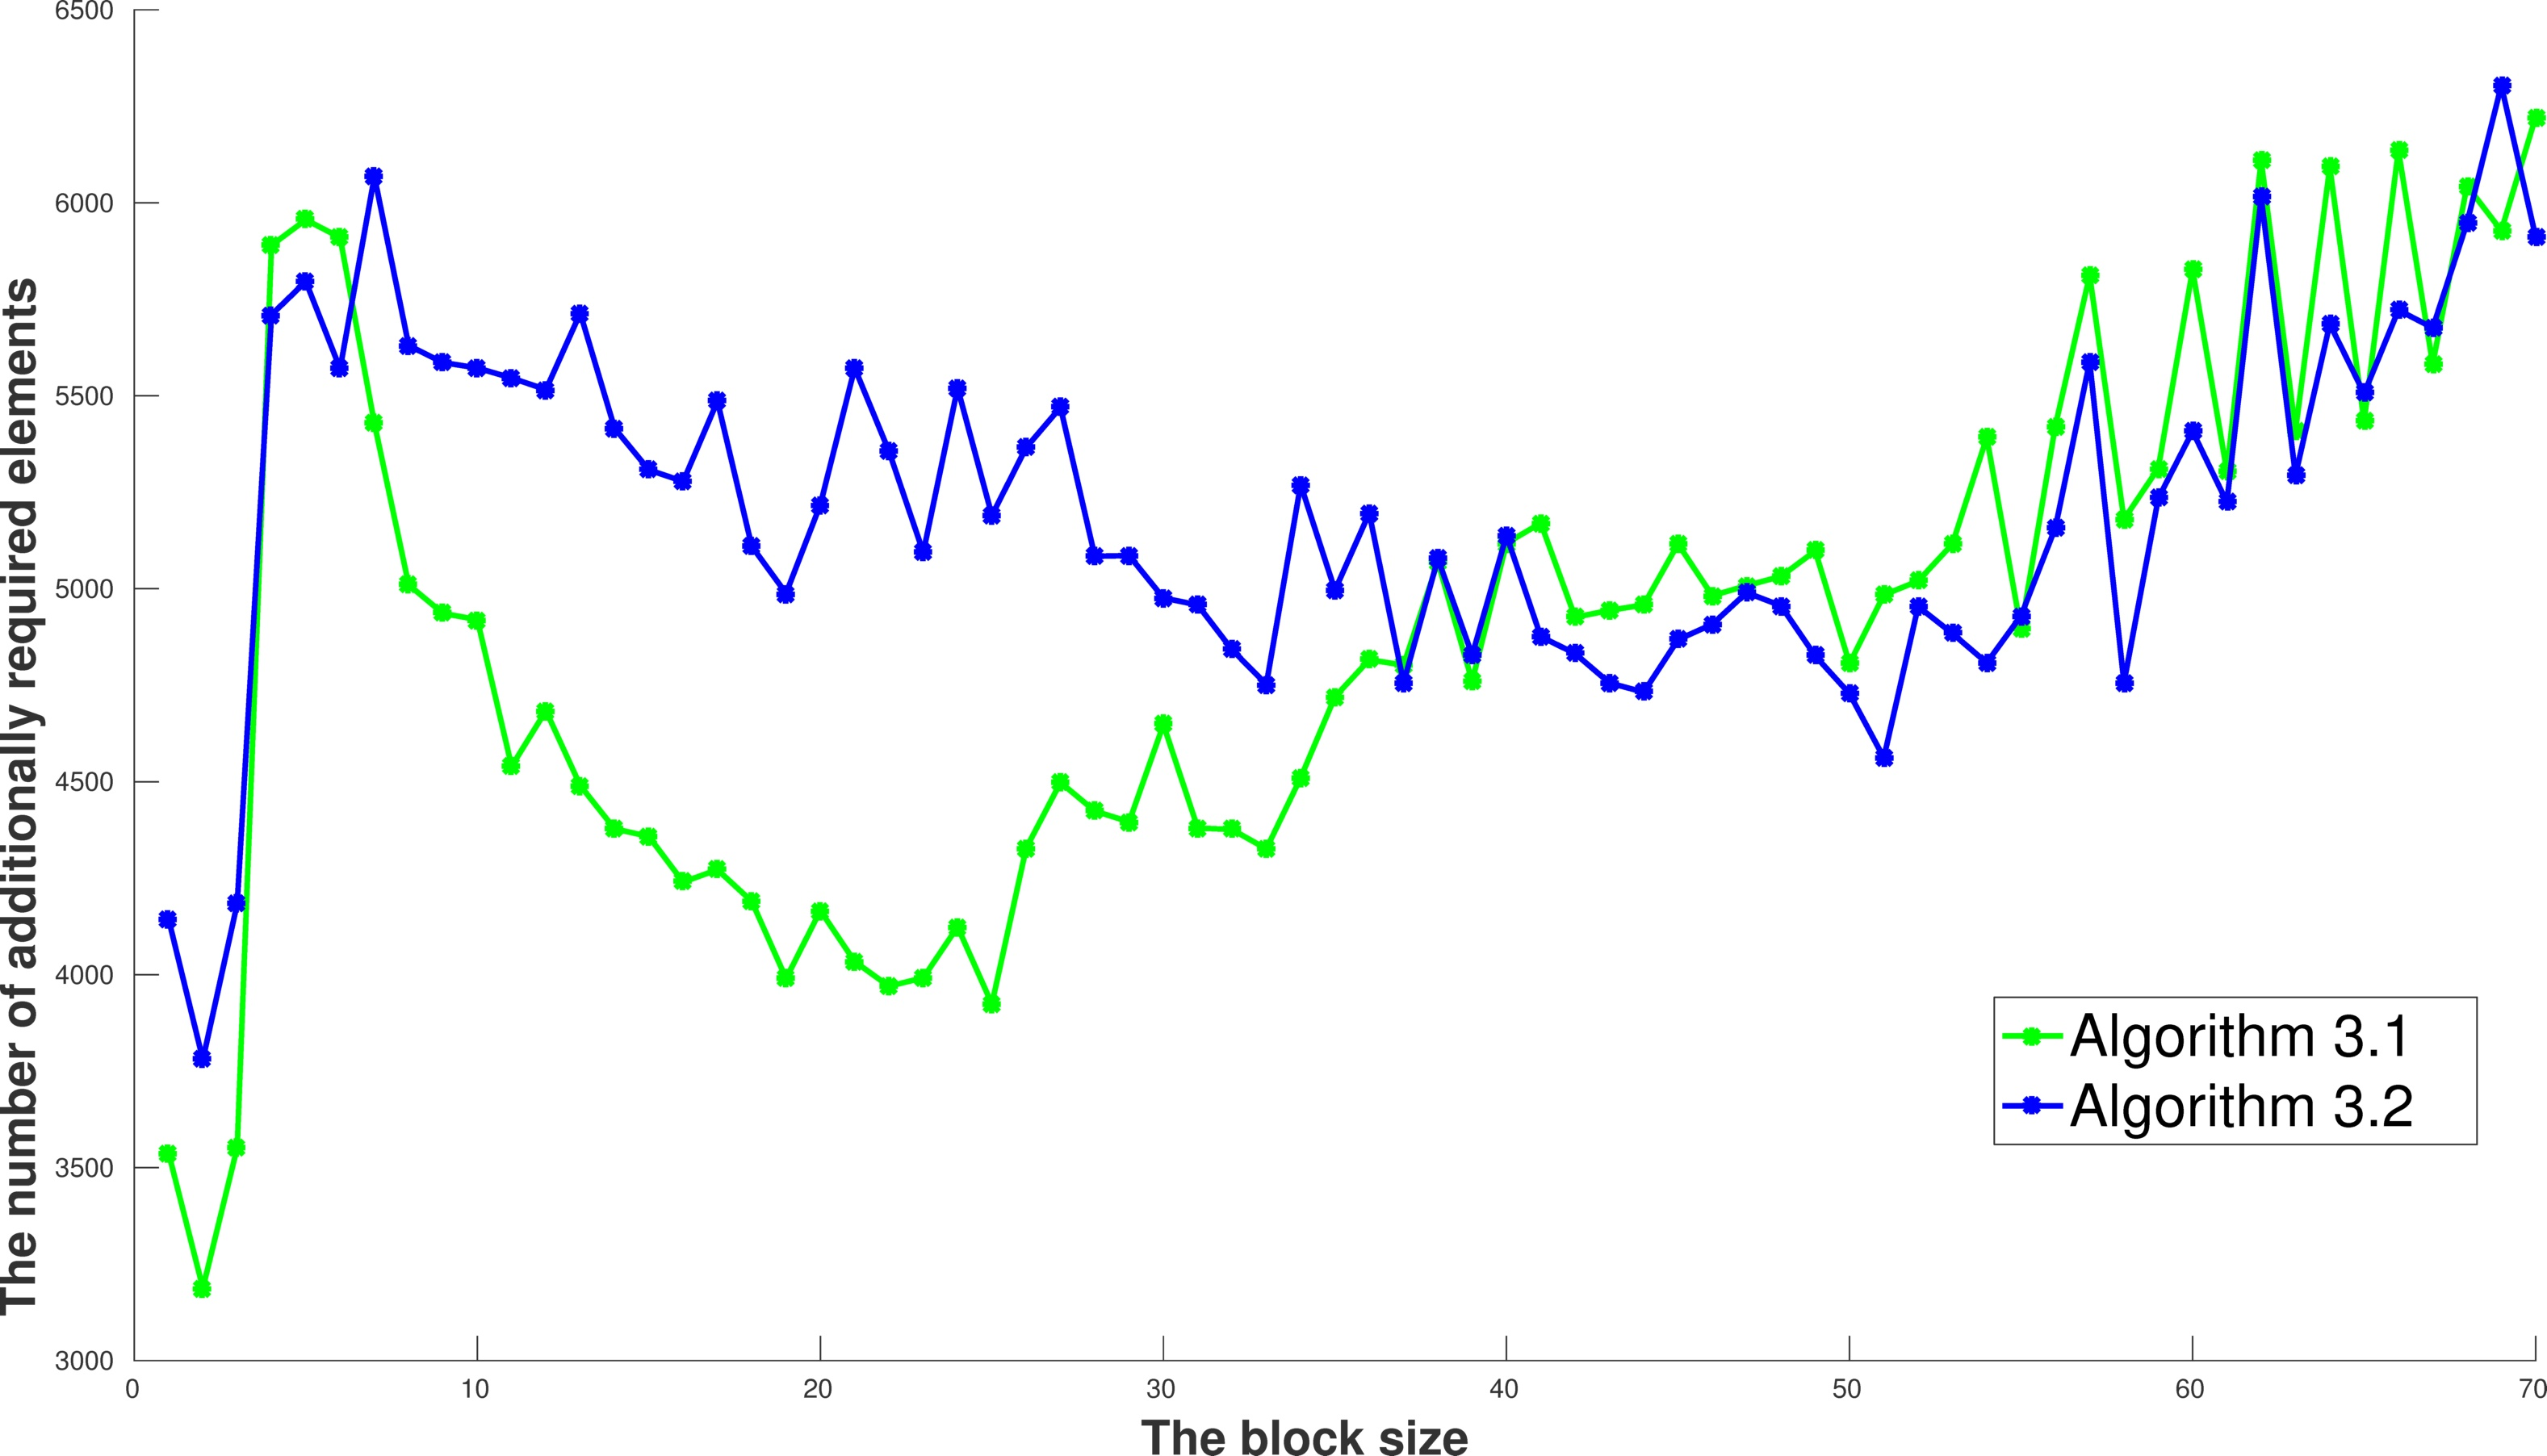
\includegraphics[width=0.9\linewidth]{ex33_alg31_alg32_bls_nat_add}
\caption{The number of additionally required elements computed by 
\coderef{code.new.d2.nreq} with the natural ordering
compared with \coderef{code.greedy}.
The computation is carried out on the matrix \textit{ex33}. }
\label{ex33_alg31_alg32_bls_nat_add}
\end{figure}

\begin{figure}
\centering
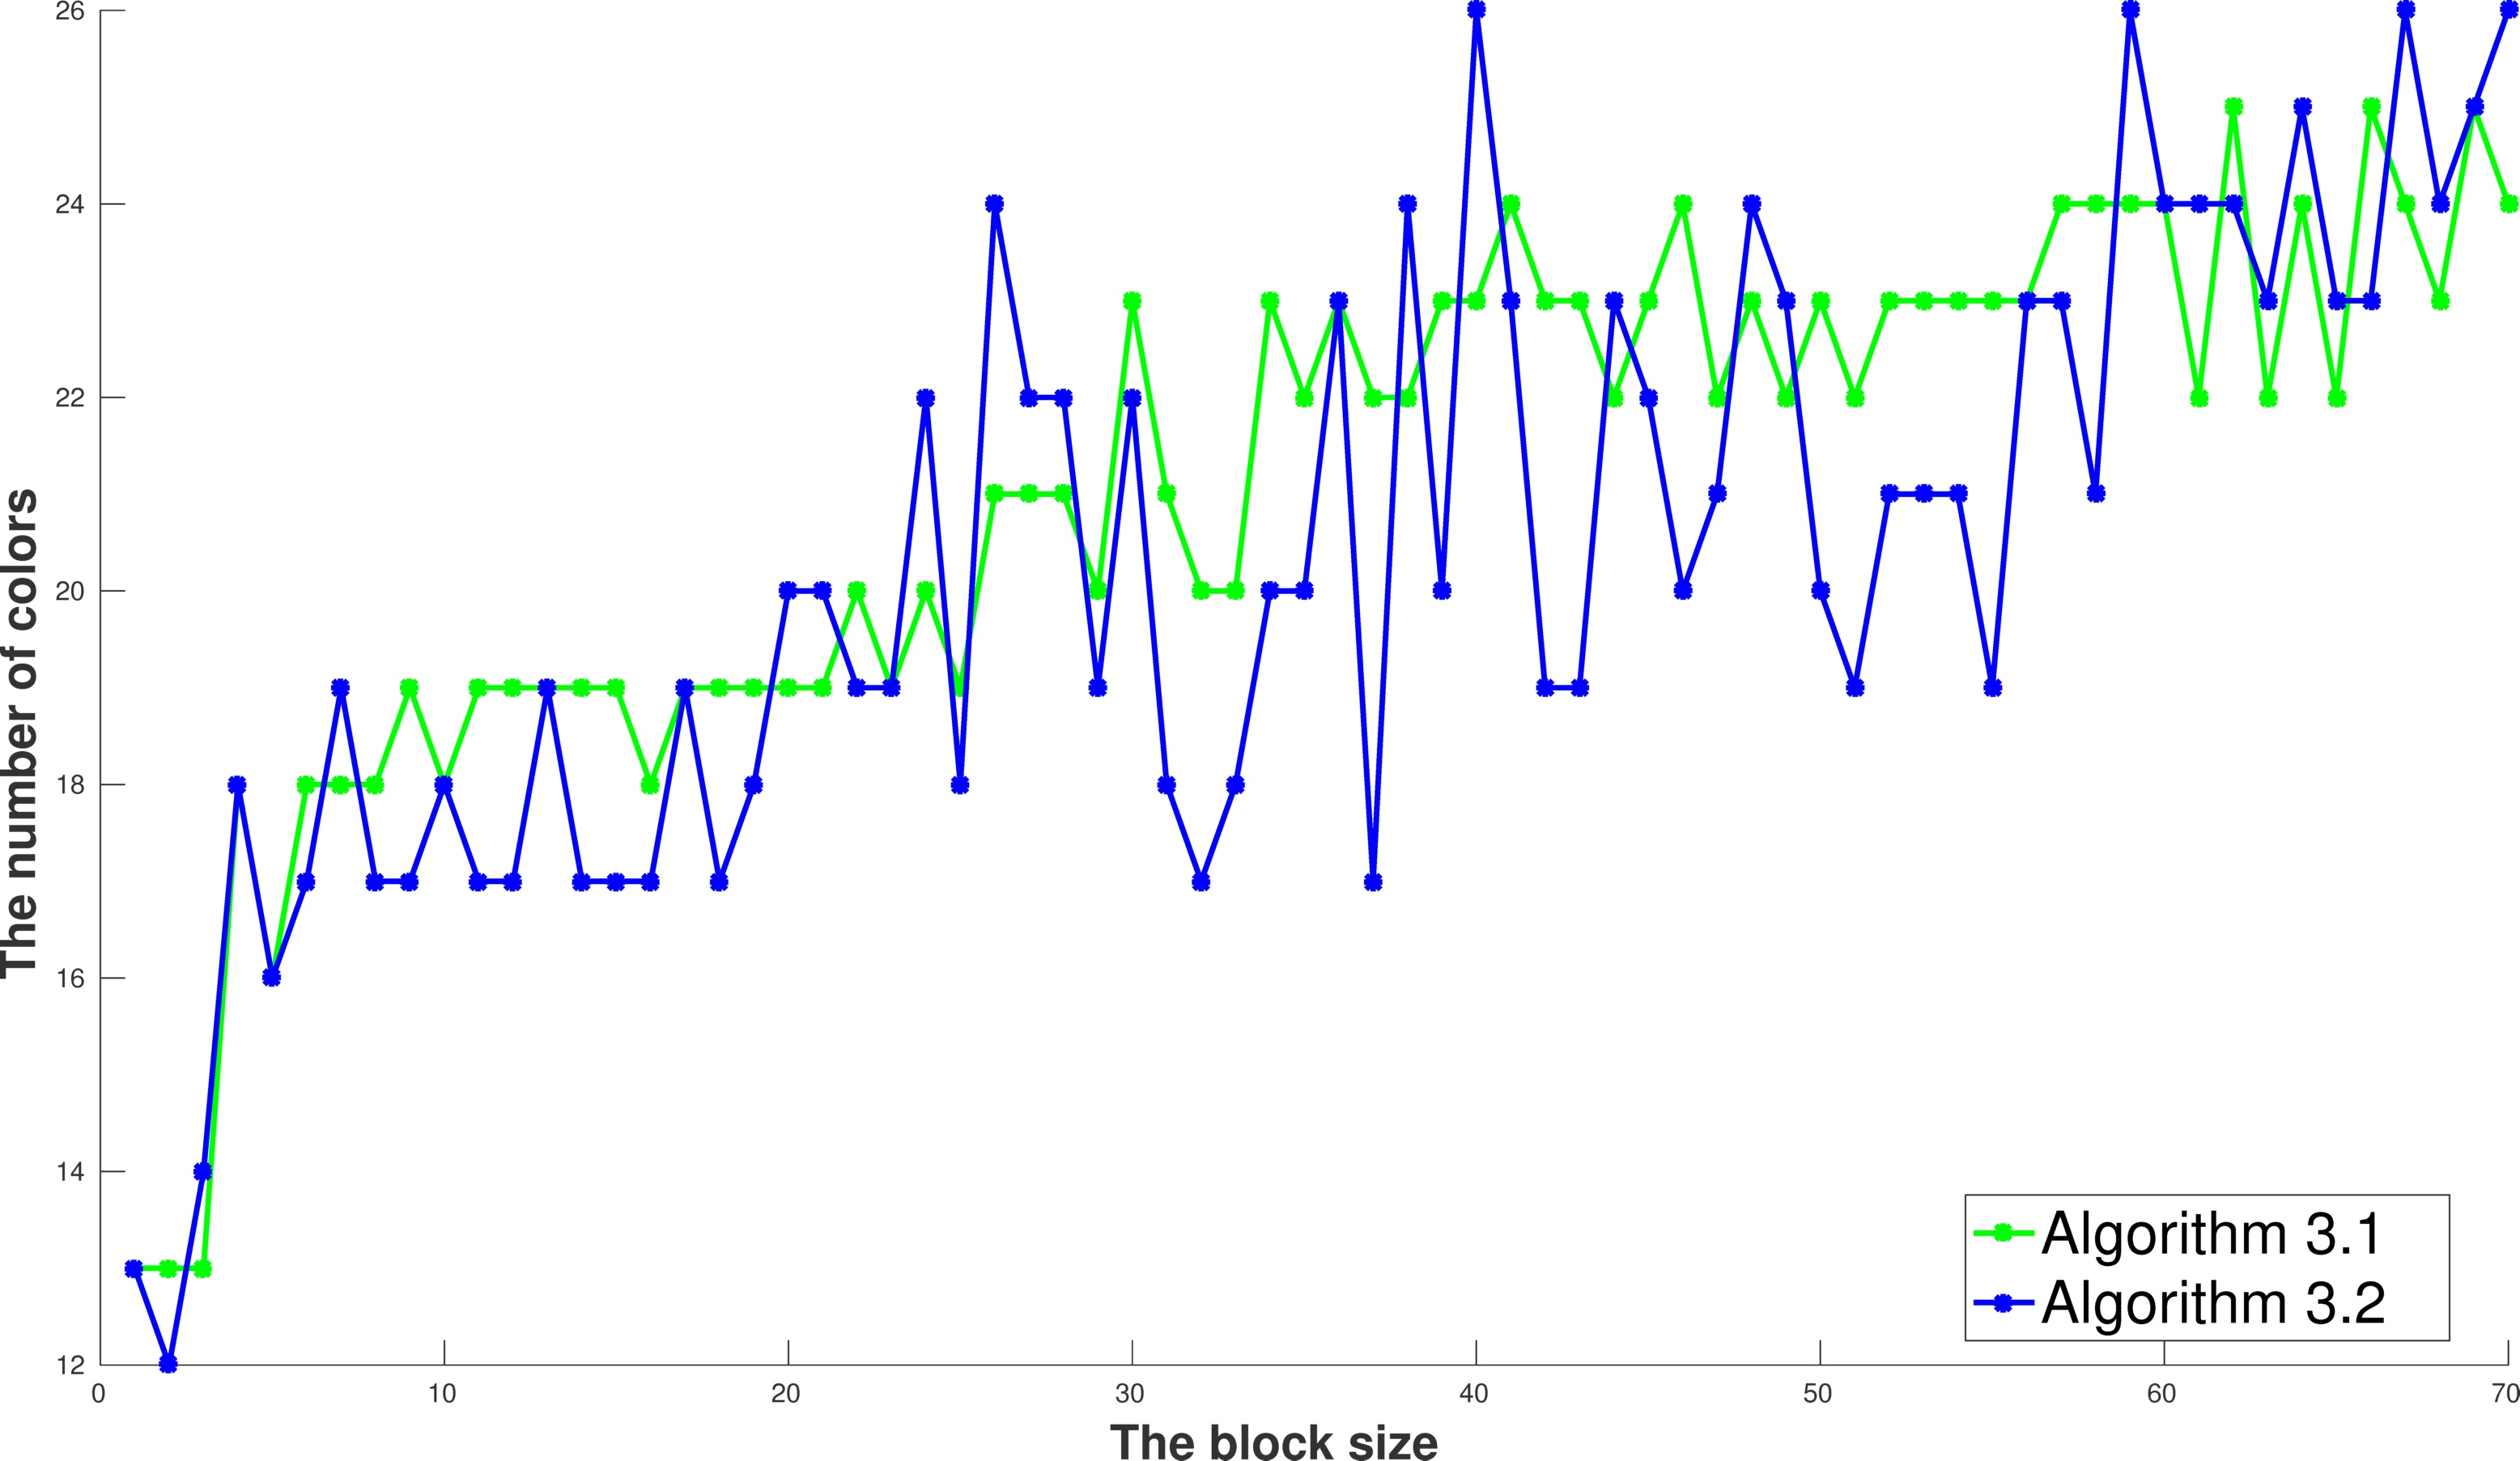
\includegraphics[width=0.9\linewidth]{ex33_alg31_alg32_bls_nat_cols}
\caption{The number of colors computed by \coderef{code.new.d2.nreq} with the natural ordering
compared with \coderef{code.greedy}. 
The computation is carried out on the matrix \textit{ex33}. }
\label{ex33_alg31_alg32_bls_nat_cols}
\end{figure}

\begin{figure}
\begin{lstlisting}[
caption=A modification of \coderef{code.new.d2.nreq} in which
a particular element is selected in lines 10 and 11.,
label=code.new.impr1,mathescape]
function d2_color_nreq_modified($G=(V_r\cup V_c,E)$,$E_i\subseteq E$)
  $\Phi\leftarrow [0\ldots 0]$
  $forbiddenColors\leftarrow [0\ldots 0]$
  for $v\in V_c$ with $N_2(v,E_i)\neq\emptyset$ and $\Phi(v)=0$
    for $n\in N_2(v,E_i)$ with $\Phi(n) \neq 0$
      $forbiddenColors[\Phi(n)] = v$
    $\Phi(v) = \min \{ a>0:forbiddenColors[a]\neq v\}$

    Determine an indepentent set $I_v$ containing $v$
    if $I_v-\{v\}\neq\emptyset$
      $maxs = \argmax_{x\in I_v - \{v\}} \nreq_v (x)$
      $mins = \argmin_{x\in maxs} \req (x)$
      $\Phi(mins[0]) = \Phi(v)$
  return $\Phi$
\end{lstlisting}
\end{figure}

\begin{figure}
\centering
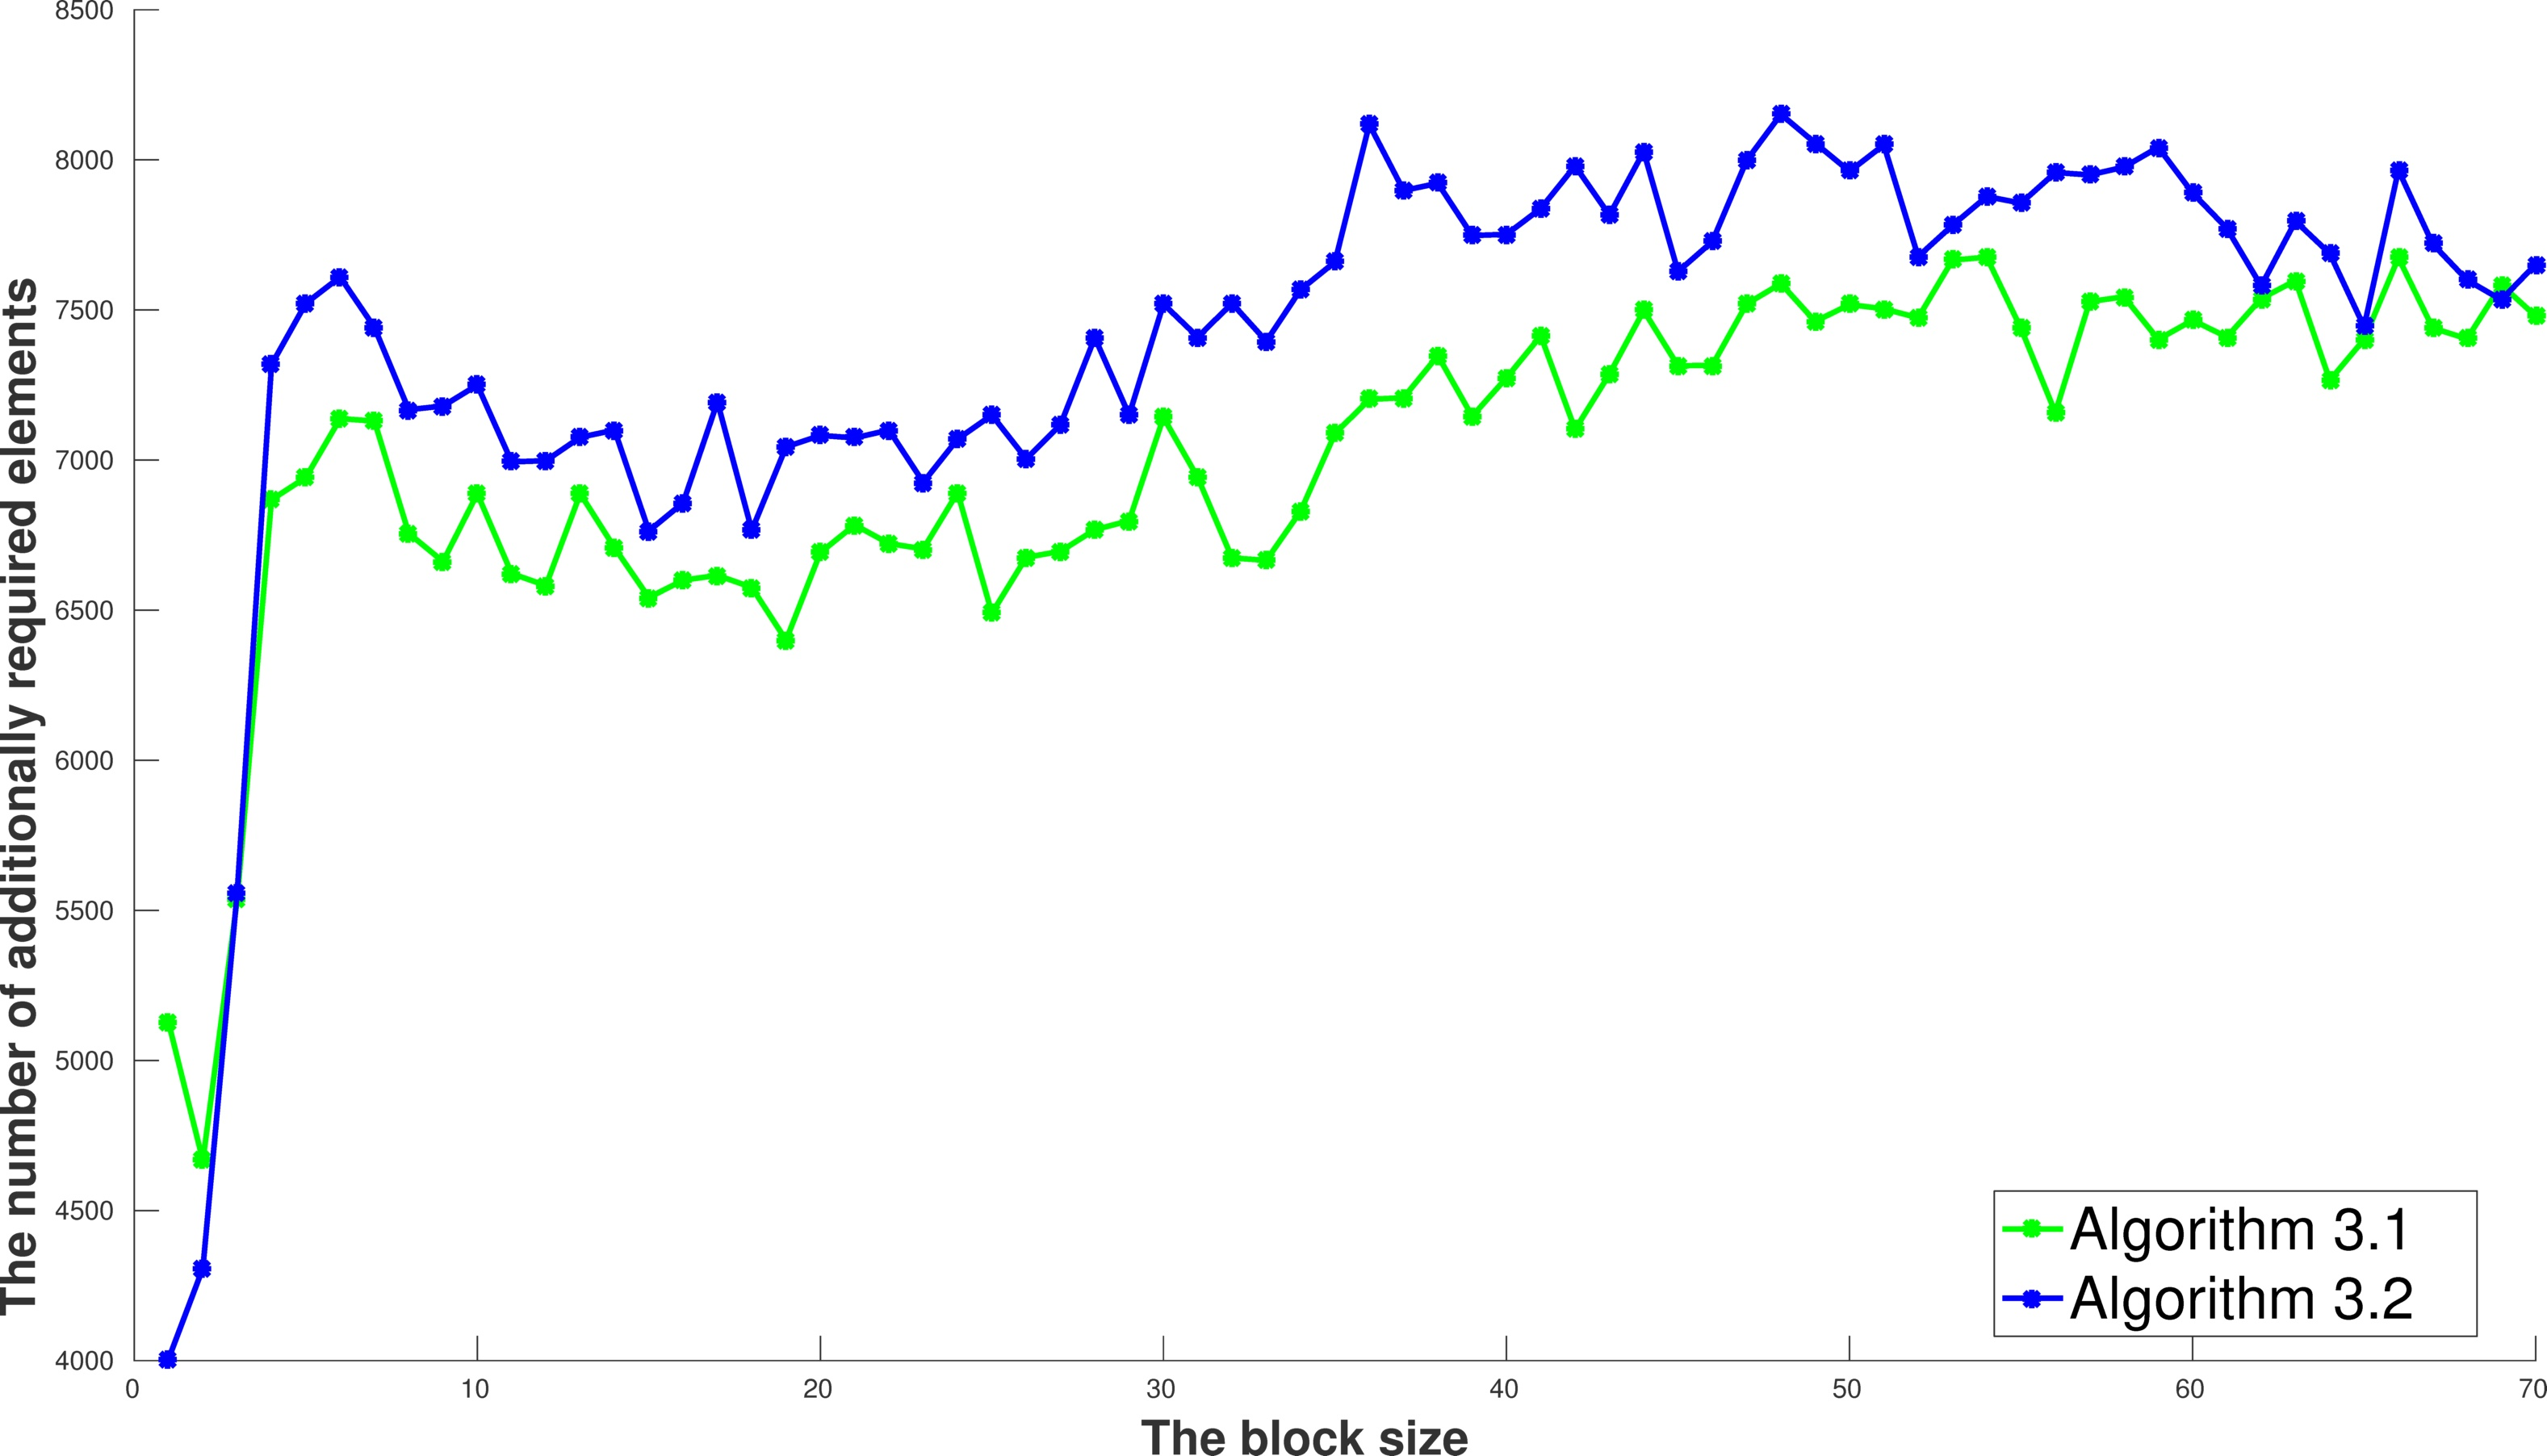
\includegraphics[width=0.9\linewidth]{ex33_alg32_alg34_bls_lfo_add}
\caption{The number of additionally
required elements are increased comparing \coderef{code.new.d2.nreq}
and \coderef{code.new.impr1} when the ordering for the coloring is the LFO ordering.
The computation is carried out on the matrix \textit{ex33}. }
\label{ex33_alg32_alg34_bls_lfo_add}
\end{figure}

Now, we modify \coderef{code.new.d2.nreq} further to select a vertex with the minimum number of 
required elements among the computed set of vertices with the maximum number of determined nonrequired elements.
This idea facilitates gathering of more nonrequired elements in the same column since
more zero elements remain. These elements might offer more options for increasing the number of determined
nonrequired elements.
Let the function $\req: V_c\rightarrow \mathbb{N}$ compute the number of required edges adjacent to a vertex.
A new algorithm is proposed in \coderef{code.new.impr1} which applies this idea. 
The only new difference of this algorithm to \coderef{code.new.d2.nreq} 
is to compute the operator $\argmin$ for the 
function $\req$. This computation has the same complexity as the computation of $\argmax$.
It means the time complexity is still as before.
\figref{ex33_alg32_alg34_bls_lfo_add} shows how the number of additionally
required elements are increased comparing
\coderef{code.new.d2.nreq} and \coderef{code.new.impr1} when the ordering for the coloring
is the LFO ordering. However, this is not the same for all matrices. 
\appref{app.compare.alg32.alg34} shows the results for different matrices
and different orderings for the block size fixed to $10$.
Except the matrix \textit{ex7}
a general observation is that the numbers of additionally and potentially required elements
are decreased when the number of colors is decreased.
This brings us to the next topic of balancing the number of colors
and the number of additioanlly required elements.

\subsubsection{Balancing the number of colors}
Here, we modify \coderef{code.new.d2.nreq} and \coderef{code.new.impr1} again 
to have a control over the balance between the number of 
colors and the number of additionally required elements.
It means we define a balance variable $\alpha \in \mathbb{N}$ such that increasing this variable 
would decrease both the number of colors and additionally required elements and vice versa.
\coderef{code.new.impr2} presents the new algorithm.
Rather than adding a single vertex as in \coderef{code.new.impr1},
the idea is to add more vertices representing columns
with the minimum number of required elements
and the maximum number of determined nonrequired elements.
This is implemented by coloring all elements of $mins$ with indices from $0$ to $\alpha-1$ .
%If the variable $\alpha=0$, we would have the same algorithm as \coderef{code.new.impr1}.
\begin{figure}
\begin{lstlisting}[
caption=New coloring heuristic with a controller to balance
the number of colors and the number of additionally required elements.,
label=code.new.impr2,mathescape]
function d2_color_nreq_balance($G=(V_r\cup V_c,E)$,$E_i\subseteq E$,$\alpha$)
  $\Phi\leftarrow [0\ldots 0]$
  $forbiddenColors\leftarrow [0\ldots 0]$
  for $v\in V_c$ with $N_2(v,E_i)\neq\emptyset$ and $\Phi(v)=0$
    for $n\in N_2(v,E_i)$ with $\Phi(n) \neq 0$
      $forbiddenColors[\Phi(n)] = v$
    $\Phi(v) = min \{ a>0:forbiddenColors[a]\neq v\}$

    Determine an indepentent set $I_v$ containing $v$
    if $I_v-\{v\}\neq\emptyset$
      $maxs = \argmax_{x\in I_v - \{v\}} \nreq_v (x)$
      $mins = \argmin_{x\in maxs} \req(x)$ 
      for $i\in\{0,1,...,\min (\alpha - 1, size(mins))\}$
        $\Phi(mins[i]) = \Phi(v)$
  return $\Phi$
\end{lstlisting}
\end{figure}

\figref{ex33_alg31_alg32_alg34_alg35_bls_lfo_cols}
shows the comparison between the number of colors computed by 
the three presented algorithms: \coderef{code.new.d2.nreq},
\coderef{code.new.impr1}, and~\coderef{code.new.impr2}.
All these algorithms are computed with the LFO ordering.
We selected this ordering for this computation 
since this ordering gives the best results.
The variable $\alpha$ for \coderef{code.new.impr2} is equal to $10$.
The block size varies also from $1$ to $80$.
It is clear from this figure that \coderef{code.new.impr2} generates the 
smallest number of colors particularly in the middle block sizes when $\alpha=10$.
However, as illustrated in \figref{ex33_alg31_alg32_alg34_alg35_bls_lfo_adds}, 
it does not perform well in the case of additionally required elements.

\begin{figure}
\centering
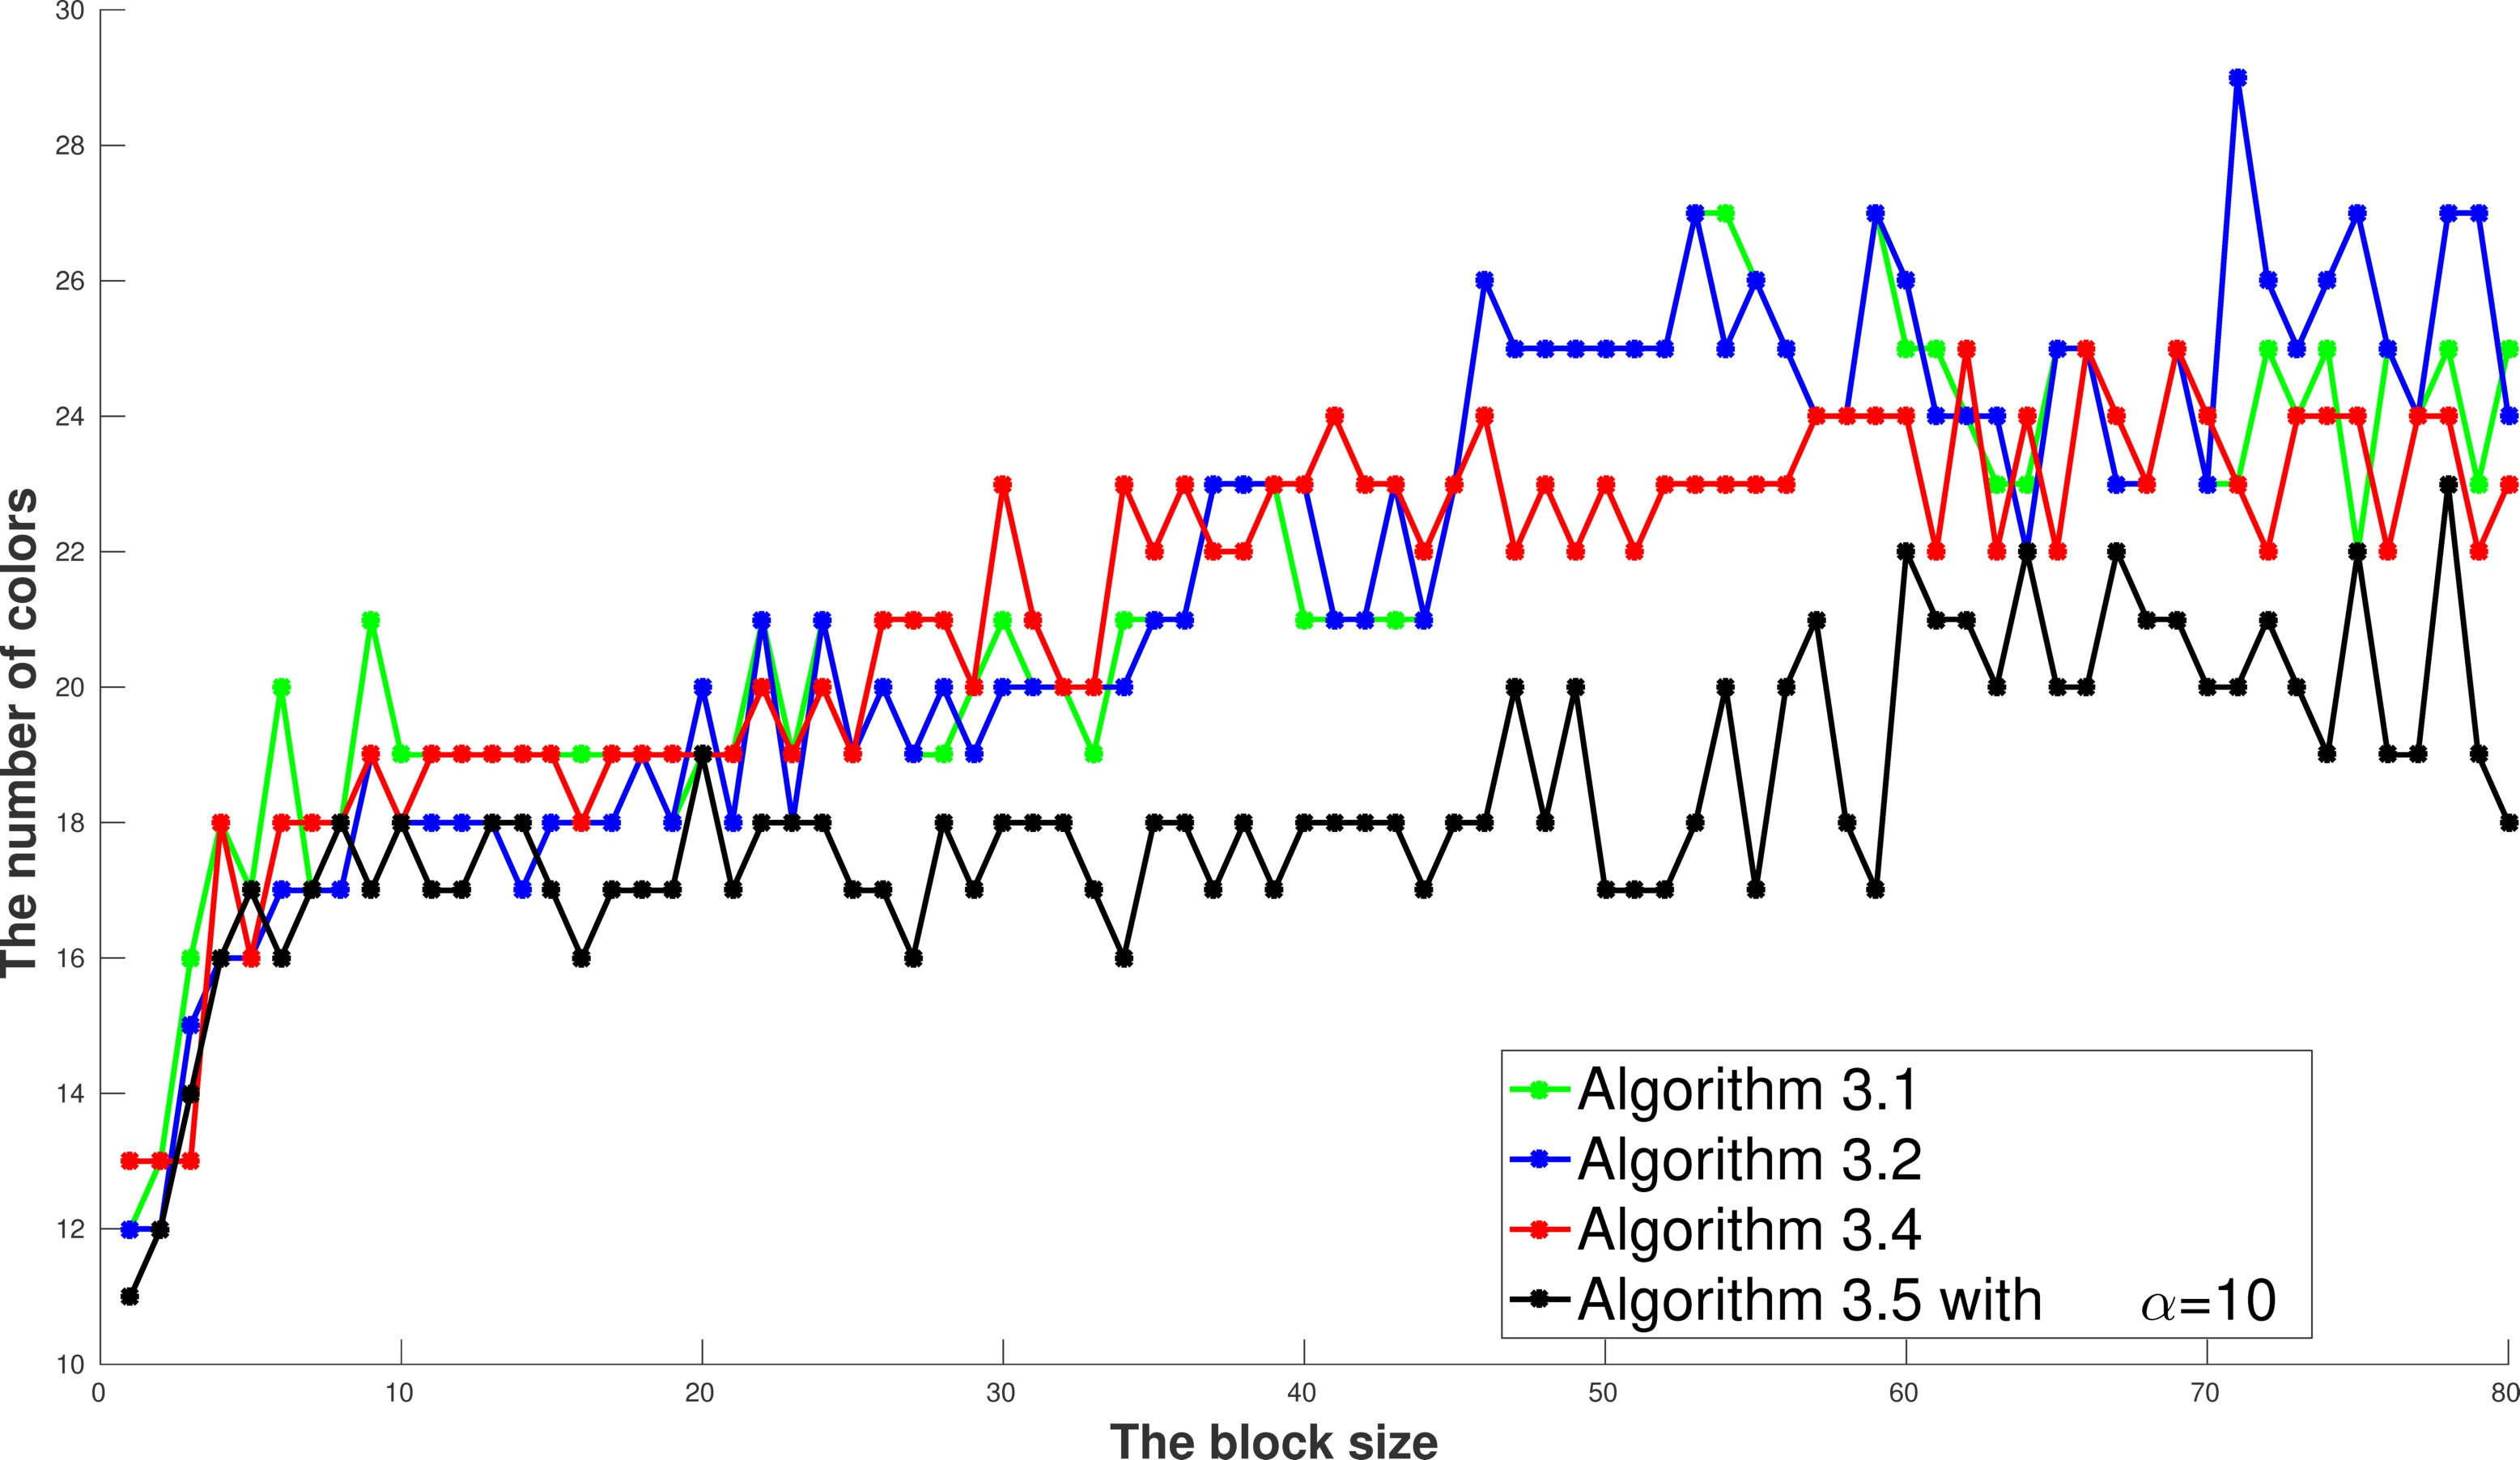
\includegraphics[width=0.9\linewidth]{ex33_alg31_alg32_alg34_alg35_bls_lfo_cols}
\caption{
The comparison of the number of colors in \coderef{code.new.d2.nreq},
\coderef{code.new.impr1}, and~\coderef{code.new.impr2}.
The computation is carried out on the matrix \textit{ex33} and with the LFO ordering.}
\label{ex33_alg31_alg32_alg34_alg35_bls_lfo_cols}
\end{figure}

\begin{figure}
\centering
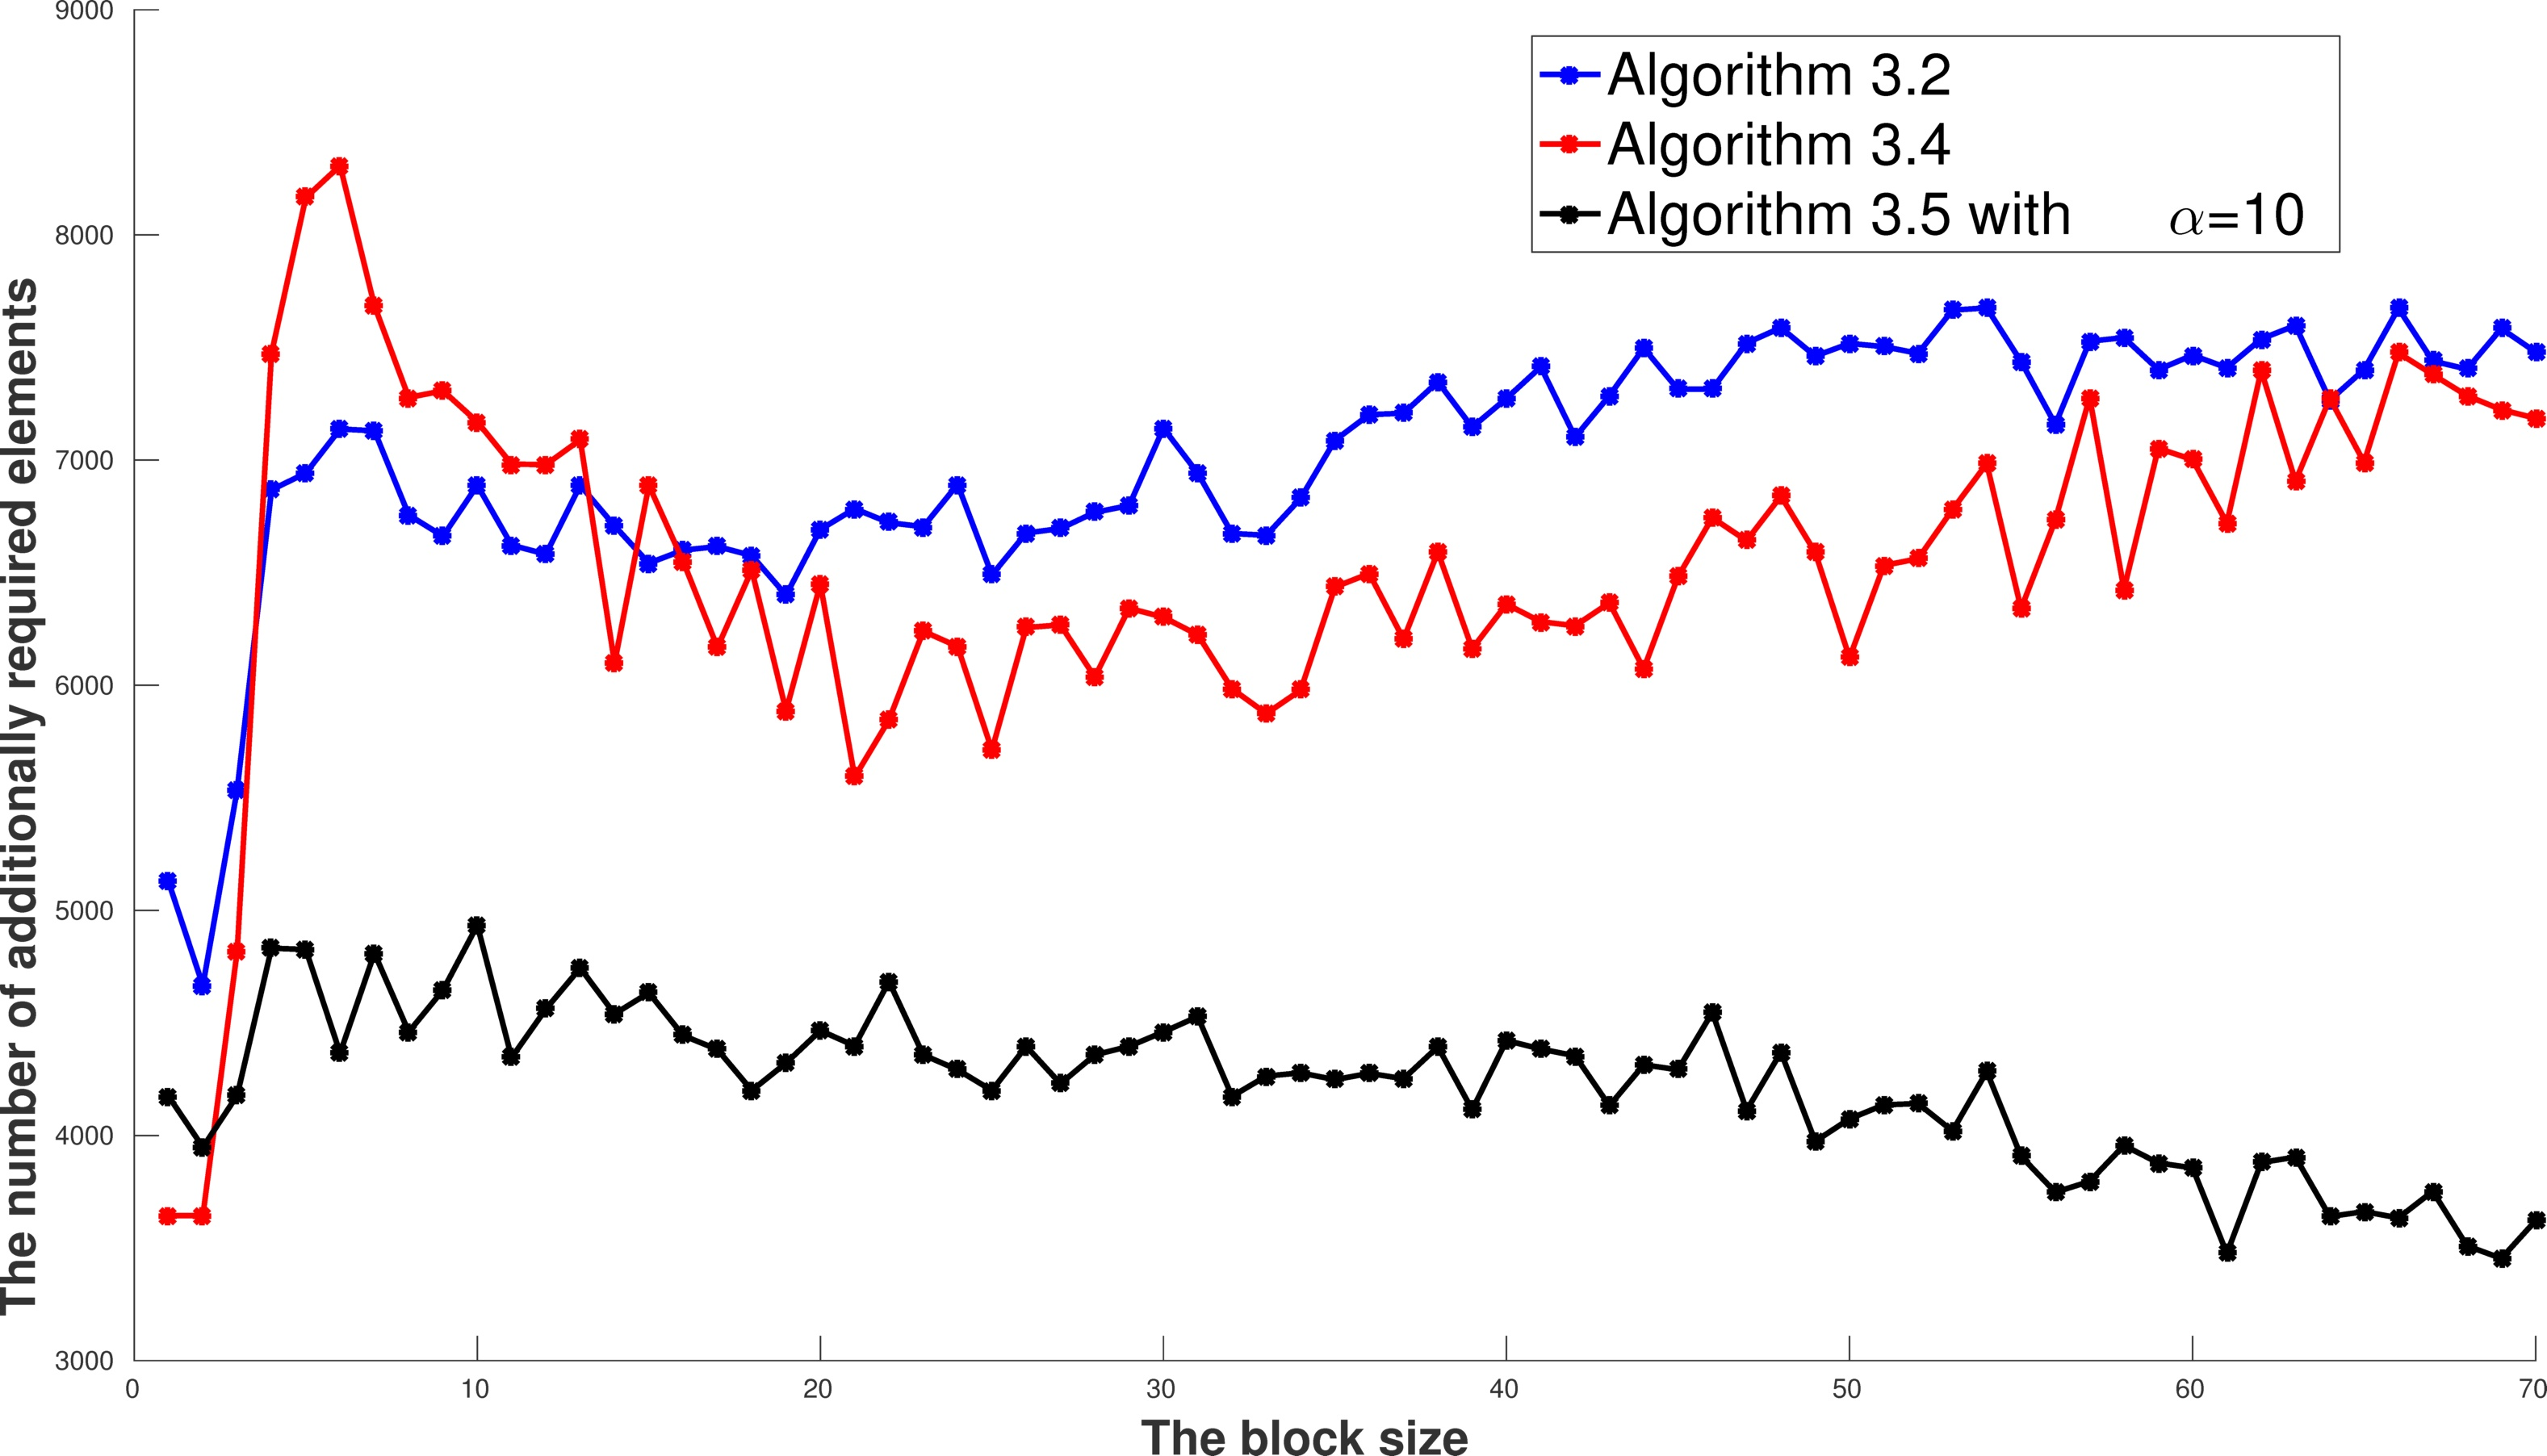
\includegraphics[width=0.9\linewidth]{ex33_alg31_alg32_alg34_alg35_bls_lfo_adds}
\caption{
The comparison of the number of additionally required elements in \coderef{code.new.d2.nreq},
\coderef{code.new.impr1}, and~\coderef{code.new.impr2}.
The computation is carried out on the matrix \textit{ex33} and with the LFO ordering.}
\label{ex33_alg31_alg32_alg34_alg35_bls_lfo_adds}
\end{figure}

Table~\ref{different.alpha} compares the number of additionally required elements and 
the number of colors using \coderef{code.new.impr2} with different $\alpha$.
Three tables at the top, middle, and the bottom of Table~\ref{different.alpha}
are for the natural ordering, the LFO ordering, and the SLO ordering, respectively.
Regardless of the ordering and except for certain cases,
the number of colors tends to decrease when $\alpha$ grows.
Indeed, the number of colors is reduced in the most of the cases. In some cases like 
the matrix \textit{steam2.mtx} with the LFO ordering, we need $6$ fewer colors comparing 
the coloring with $\alpha=0$ and $\alpha=10$.

On the other hand, except for certain cases, 
the number of additionally required elements decreases 
when $\alpha$ increases in the coloring.
However, in this table,
the coloring with $\alpha=6$ can be a suitable choice in most of the cases
since the number of additionally required elements is relatively high
while the number of colors is mainly small.
More figures can be found in \appref{app.compare.alg35.alphas} comparing these values
based on the varying block sizes.

\begin{table}
\centering
\begin{tabular}{|c|c|c|c|c|c|c|}
\hline
Matrix (NAT) & \multicolumn{6}{c|}{\coderef{code.new.impr2}} \\\hline
{} & \multicolumn{3}{c|}{$|R_{a}|$} & \multicolumn{3}{c|}{$|\Phi|$}\\\hline
{}     & $\alpha=0$ & $\alpha=6$ & $\alpha=10$ & $\alpha=0$& $\alpha=6$&$\alpha=10$ \\\hline
\textit{steam1.mtx} & $566$ & $440$ & $370$ & $10$ & $9$ & $8$ \\\hline
\textit{steam2.mtx} & $1512$ & $944$ & $1032$ & $13$ & $10$ & $9$ \\\hline
\textit{nos3.mtx} & $3416$ & $2778$ & $2348$ & $20$ & $18$ & $17$ \\\hline
\textit{ex7.mtx} & $23958$ & $22656$ & $21180$ & $55$ & $49$ & $46$ \\\hline
\textit{ex33.mtx} & $5992$ & $5616$ & $5262$ & $19$ & $18$ & $18$ \\\hline
\textit{crystm01.mtx} & $28348$ & $28466$ & $28516$ & $22$ & $24$ & $24$ \\\hline
\textit{coater1.mtx} & $7896$ & $7562$ & $7538$ & $30$ & $26$ & $25$ \\\hline
\end{tabular}
\vspace*{1cm}\newline
\begin{tabular}{|c|c|c|c|c|c|c|}
\hline
Matrix (LFO) & \multicolumn{6}{c|}{\coderef{code.new.impr2}} \\\hline
{} & \multicolumn{3}{c|}{$|R_{a}|$} & \multicolumn{3}{c|}{$|\Phi|$}\\\hline
{} & $\alpha=0$ & $\alpha=6$ & $\alpha=10$ & $\alpha=0$& $\alpha=6$&$\alpha=10$ \\\hline
\textit{steam1.mtx} & $518$ & $456$ & $330$ & $12$ & $10$ & $10$ \\\hline
\textit{steam2.mtx} & $1280$ & $660$ & $564$ & $17$ & $13$ & $11$ \\\hline
\textit{nos3.mtx} & $3646$ & $2360$ & $2190$ & $20$ & $19$ & $19$ \\\hline
\textit{ex7.mtx} & $22532$ & $21444$ & $21576$ & $49$ & $48$ & $47$ \\\hline
\textit{ex33.mtx} & $5968$ & $5222$ & $4934$ & $16$ & $17$ & $16$ \\\hline
\textit{crystm01.mtx} & $21168$ & $21918$ & $21210$ & $18$ & $18$ & $18$ \\\hline
\textit{coater1.mtx} & $7210$ & $7168$ & $6998$ & $23$ & $23$ & $23$ \\\hline
\end{tabular}
\vspace*{1cm}\newline
\begin{tabular}{|c|c|c|c|c|c|c|}
\hline
Matrix (SLO) & \multicolumn{6}{c|}{\coderef{code.new.impr2}} \\\hline
{} & \multicolumn{3}{c|}{$|R_{a}|$} & \multicolumn{3}{c|}{$|\Phi|$}\\\hline
{} & $\alpha=0$ & $\alpha=6$ & $\alpha=10$ & $\alpha=0$& $\alpha=6$&$\alpha=10$ \\\hline
\textit{steam1.mtx} & $748$ & $476$ & $390$ & $14$ & $13$ & $13$ \\\hline
\textit{steam2.mtx} & $1816$ & $1024$ & $980$ & $17$ & $12$ & $11$ \\\hline
\textit{nos3.mtx} & $3998$ & $2620$ & $1978$ & $20$ & $18$ & $17$ \\\hline
\textit{ex7.mtx} & $23598$ & $22362$ & $22098$ & $52$ & $50$ & $49$ \\\hline
\textit{ex33.mtx} & $6174$ & $5752$ & $4902$ & $19$ & $18$ & $17$ \\\hline
\textit{crystm01.mtx} & $27432$ & $26478$ & $27782$ & $22$ & $22$ & $22$ \\\hline
\textit{coater1.mtx} & $7668$ & $7624$ & $7570$ & $25$ & $26$ & $24$ \\\hline
\end{tabular}
\caption{The comparison of the additionally required elements and the number of colors 
in the computation of \coderef{code.new.impr2} with the different value of $\alpha$.
The orderings for coloring are (Top) the natural ordering,
(Middle) LFO, and (Bottom) SLO.}
\label{different.alpha}
\end{table}


%%%%%%%%%%%%%%%%%%%%%%%%%%%%%%%%%%%%%%%%%%%%%%%%%%%%%%%%%%%%%%%%%%%%%%%%%%%%%%%%%%%%%%%%%
\clearpage
\subsection{Restricted star bicoloring}
\label{s.heuristic.starbicoloring}
%%%%%%%%%%%%%%%%%%%%%%%%%%%%%%%%%%%%%%%%%%%%%%%%%%%%%%%%%%%%%%%%%%%%%%%%%%%%%%%%%%%%%%%%%%
Here, we search for a modified version of star bicoloring
which increases the number of potentially and additionally required elements without
a high increase in the number of colors.
We can apply the ideas from \coderef{code.new.impr1} and \coderef{code.new.impr2}.
However, we should not expect to have a high increase of the number of additionally required elements
equal to the sum of the increases in the column compression and row compression.

The classical approach toward star bicoloring is first introduced in
\cite{Gebremedhin05whatcolor} as star bicoloring scheme.
Lülfesmann~\cite{LulfesmannMaster} is implemented and evaluated this algorithm.
This algorithm performs convincing since the steps of the algorithms is near to the definition of the coloring.
Complete direct solver bicoloring and Row/Column Fill Bicoloring~\cite{Hossain95computinga}
are the other algorithms which are introduced for bicoloring.
As Calotoiu~\cite{CalotoiuMaster} discusses theses algorithms do not perform
better than the classic star bicoloring scheme.
Also, Calotoiu~\cite{CalotoiuMaster} introduces the integrated star bicoloring
and total ordering star bicoloring which performs better than
star bicoloring scheme in some matrices and not much worse in some other matrices.

We consider the implementation of star bicoloring in \coderef{orig.star.bicoloring} based on
the algorithm from Lülfesmann~\cite{Lulfesmann2012Fap}.
Here, the notation $G[S]$ means the graph induces on the edge set $S$.
Also, the notation $\Delta(V,G)$ represents the maximum degree of the vertices from $V$ and in the graph $G$.
This algorithm in lines $7$ to $10$ selects first which vertex should be processed in the next step.
Should it be from the column vertices or the row vertices?
This selection is based on the value of $\rho$ and the maximum degree of vertices in each step.
After this selection, the conditions of the star bicoloring is analyzed in the next lines of algorithm.
The lines $25$ and $26$ are just postprocessing steps which make the colors distinct for the column and
row vertices. Finally, we color the uncolored vertices with the color $0$ in lines $27$ and $28$.
\begin{figure}
\begin{lstlisting}[
caption=The heuristic from Lülfesmann~\cite{Lulfesmann2012Fap} for star bicoloring.,
label=orig.star.bicoloring,mathescape]
function star_bicoloring($G=(V_r\cup V_c,E)$,$E_i\subseteq E$,$\rho$)
  $\Phi\leftarrow [-1\ldots -1]$
  $forbiddenColors\leftarrow [0\ldots 0]$
  $E_i^{'} = E_i$
  $v = 0$
  while $E_i^{'}\neq\emptyset$
    if($\Delta(V_r,G[E_i^{'}]) > \rho \Delta(V_c,G[E_i^{'}])$ then
      $v$ = $v_r\in V_r$ with maximum degree in $G[E_i^{'}]$
    else
      $v$ = $v_c\in V_c$ with maximum degree in $G[E_i^{'}]$
    $E_i^{'} = E_i^{'} - \{(v,w)\in E_i^{'}:w\in N_1(v,G[E_i^{'}])\}$
    for $w\in N_1(v,G)$
      if $\Phi(w) \leq 0$
        for $x\in N_1(w,G)$ with $\Phi(w) > 0$
          if $(v,w) \in E_i$ or $(w,x) \in E_i$
            $forbiddenColors[\Phi (x)]=v$
      else
        for $x\in N_1(w,G[E_i])$ with $\Phi(x) > 0$
        for $y\in N_1(x,G)$ with $\Phi(y) > 0$ and $y\neq w$
          if $\Phi(w) = \Phi(y)$
            $forbiddenColors[\Phi (x)] = v$
            
    $\Phi(v) = min(\{j>0: forbiddenColors[j] \neq v\})$

  for $v_c\in V_c$ with $\Phi(v_c) > 0$
    $\Phi (v_c) = \Phi (v_c) + max(\{\Phi (v_r): v_r \in V_r\})$

  for $v\in V_r\cup V_c$ with $\Phi(v)= -1$
    $\Phi (v) = 0$

  return $\Phi$
\end{lstlisting}

\begin{lstlisting}[
caption= Our new heuristic for star bicoloring considering the determined nonrequired elements.,
label=new.star.bicoloring,mathescape]
function star_bicoloring_nreq($G=(V_r\cup V_c,E)$,$E_i\subseteq E$,$\rho$)
  $...$
  $NonReq=false$
  while $E_i^{'}\neq\emptyset$
    if NonReq = false
      if $\Delta(V_r,G[E_i^{'}]) > \rho \Delta(V_c,G[E_i^{'}]$ then
        $v$ = $v_r\in V_r$ with maximum degree in $G[E_i^{'}]$
      else
        $v$ = $v_c\in V_c$ with maximum degree in $G[E_i^{'}]$
      $NonReq=true$
    else
      Determine an indepentent set $I_v$ containing $v$
      if $I_v-\{v\}\neq\emptyset$
        $maxs = \argmax_{x\in I_v - \{v\}} \nreq_v (x)$
        $mins = \argmin_{x\in maxs} \req(x)$ 
        $v=mins[0]$
      $NonReq=false$
    $E_i^{'} = E_i^{'} - \{(v,w)\in E_i^{'}:w\in N_1(v,G[E_i^{'}])\}$
  $...$
  return $\Phi$
\end{lstlisting}
\end{figure}

Before introducing our new heuristic, 
we first do computations to find the influence of $\rho$ on the
number of additionally required elements.
The value of $\rho$ is a weightening factor which
is a balance between columns or row vertices. A higher value of $\rho$
makes the compression mostly in the column vertices and vice versa.
There are some discussion on how to choose the value of $\rho$ in
\cite{Gebremedhin05whatcolor}. Also,
Lülfesmann~\cite{Lulfesmann2012Fap,LulfesmannMaster} did some computation for some specific $\rho$.
However, the goal in the previous literature is to minimize the number of colors.
As the \figref{rho_value_685_bus} and \figref{rho_value_orani678},
the value of $\rho$ has a direct influence on
the number of additionally required elements.
The interesting observation is that a tiny change
on the value of $\rho$ can dramatically change the
results. For example, changing the value of $\rho$ from
$0.3$ to $0.4$ in \figref{rho_value_orani678} would result
in a change of $10000$ in the number of additionally required elements.

\begin{figure}
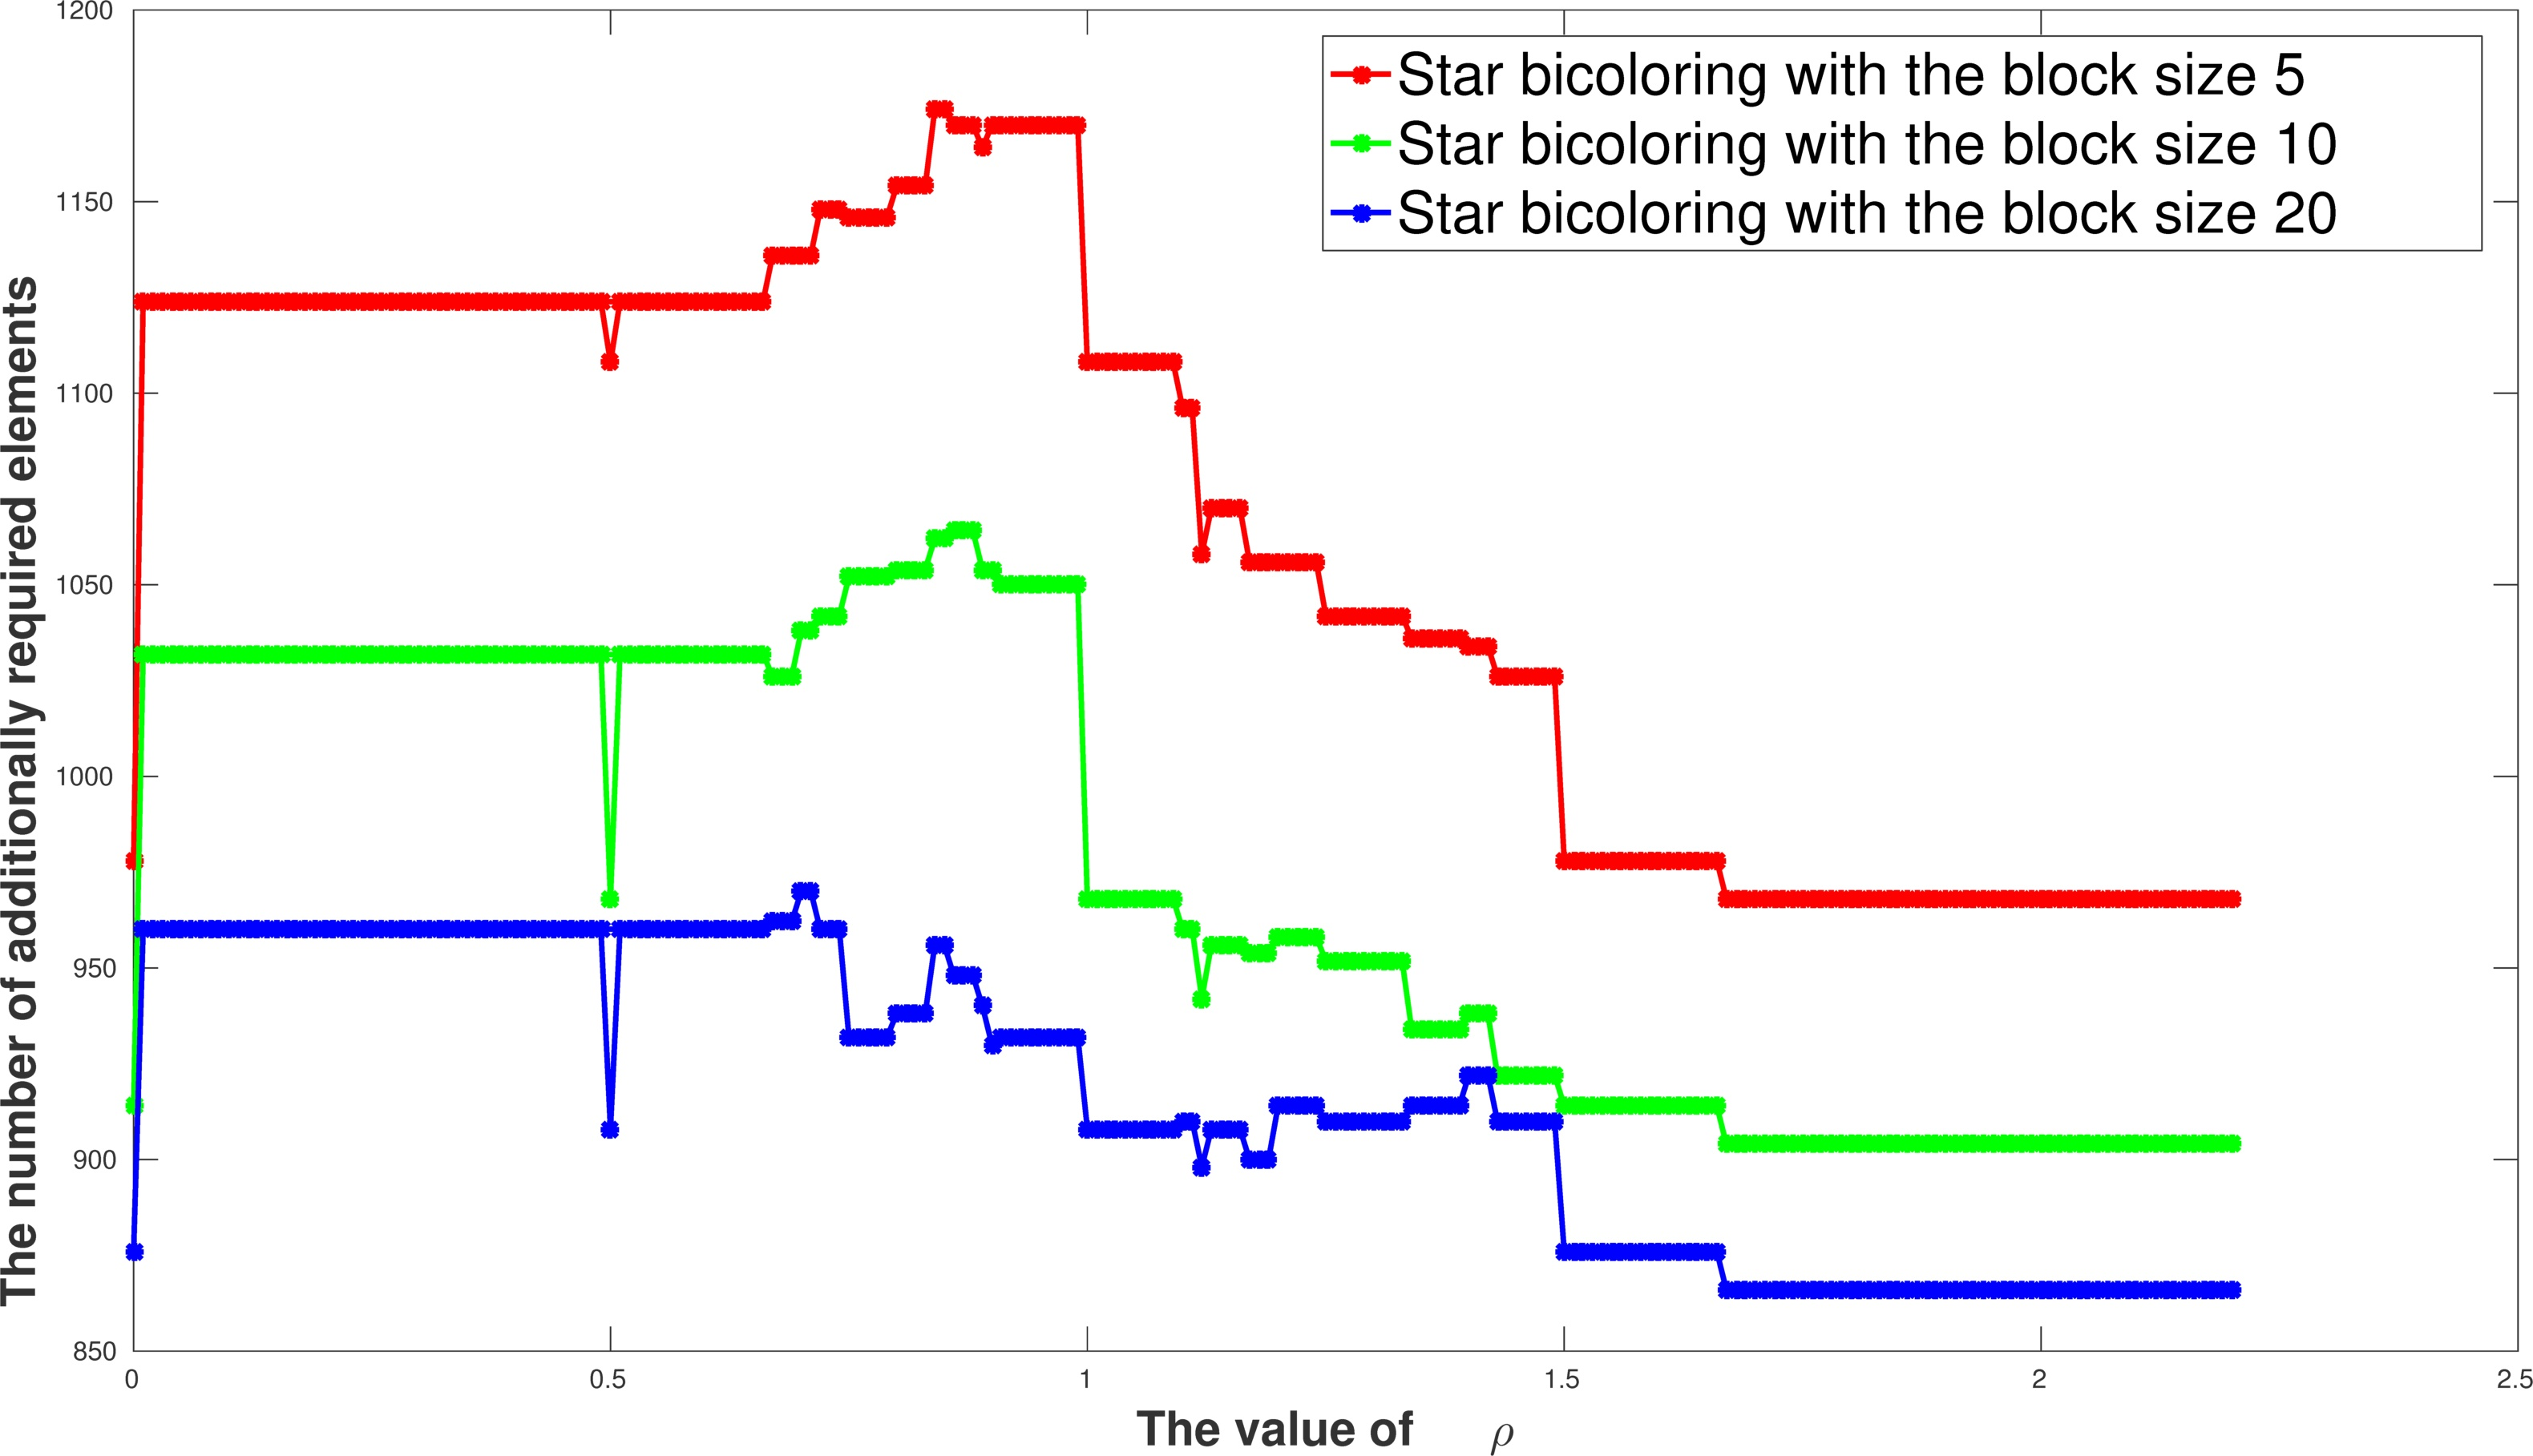
\includegraphics[width=0.9\linewidth]{rho_value_685_bus}
\caption{The influence of $\rho$ is computed on the additionally required elements
for the matrix \textit{685\_bus} with the LFO ordering.}
\label{rho_value_685_bus}
\end{figure}

\begin{figure}
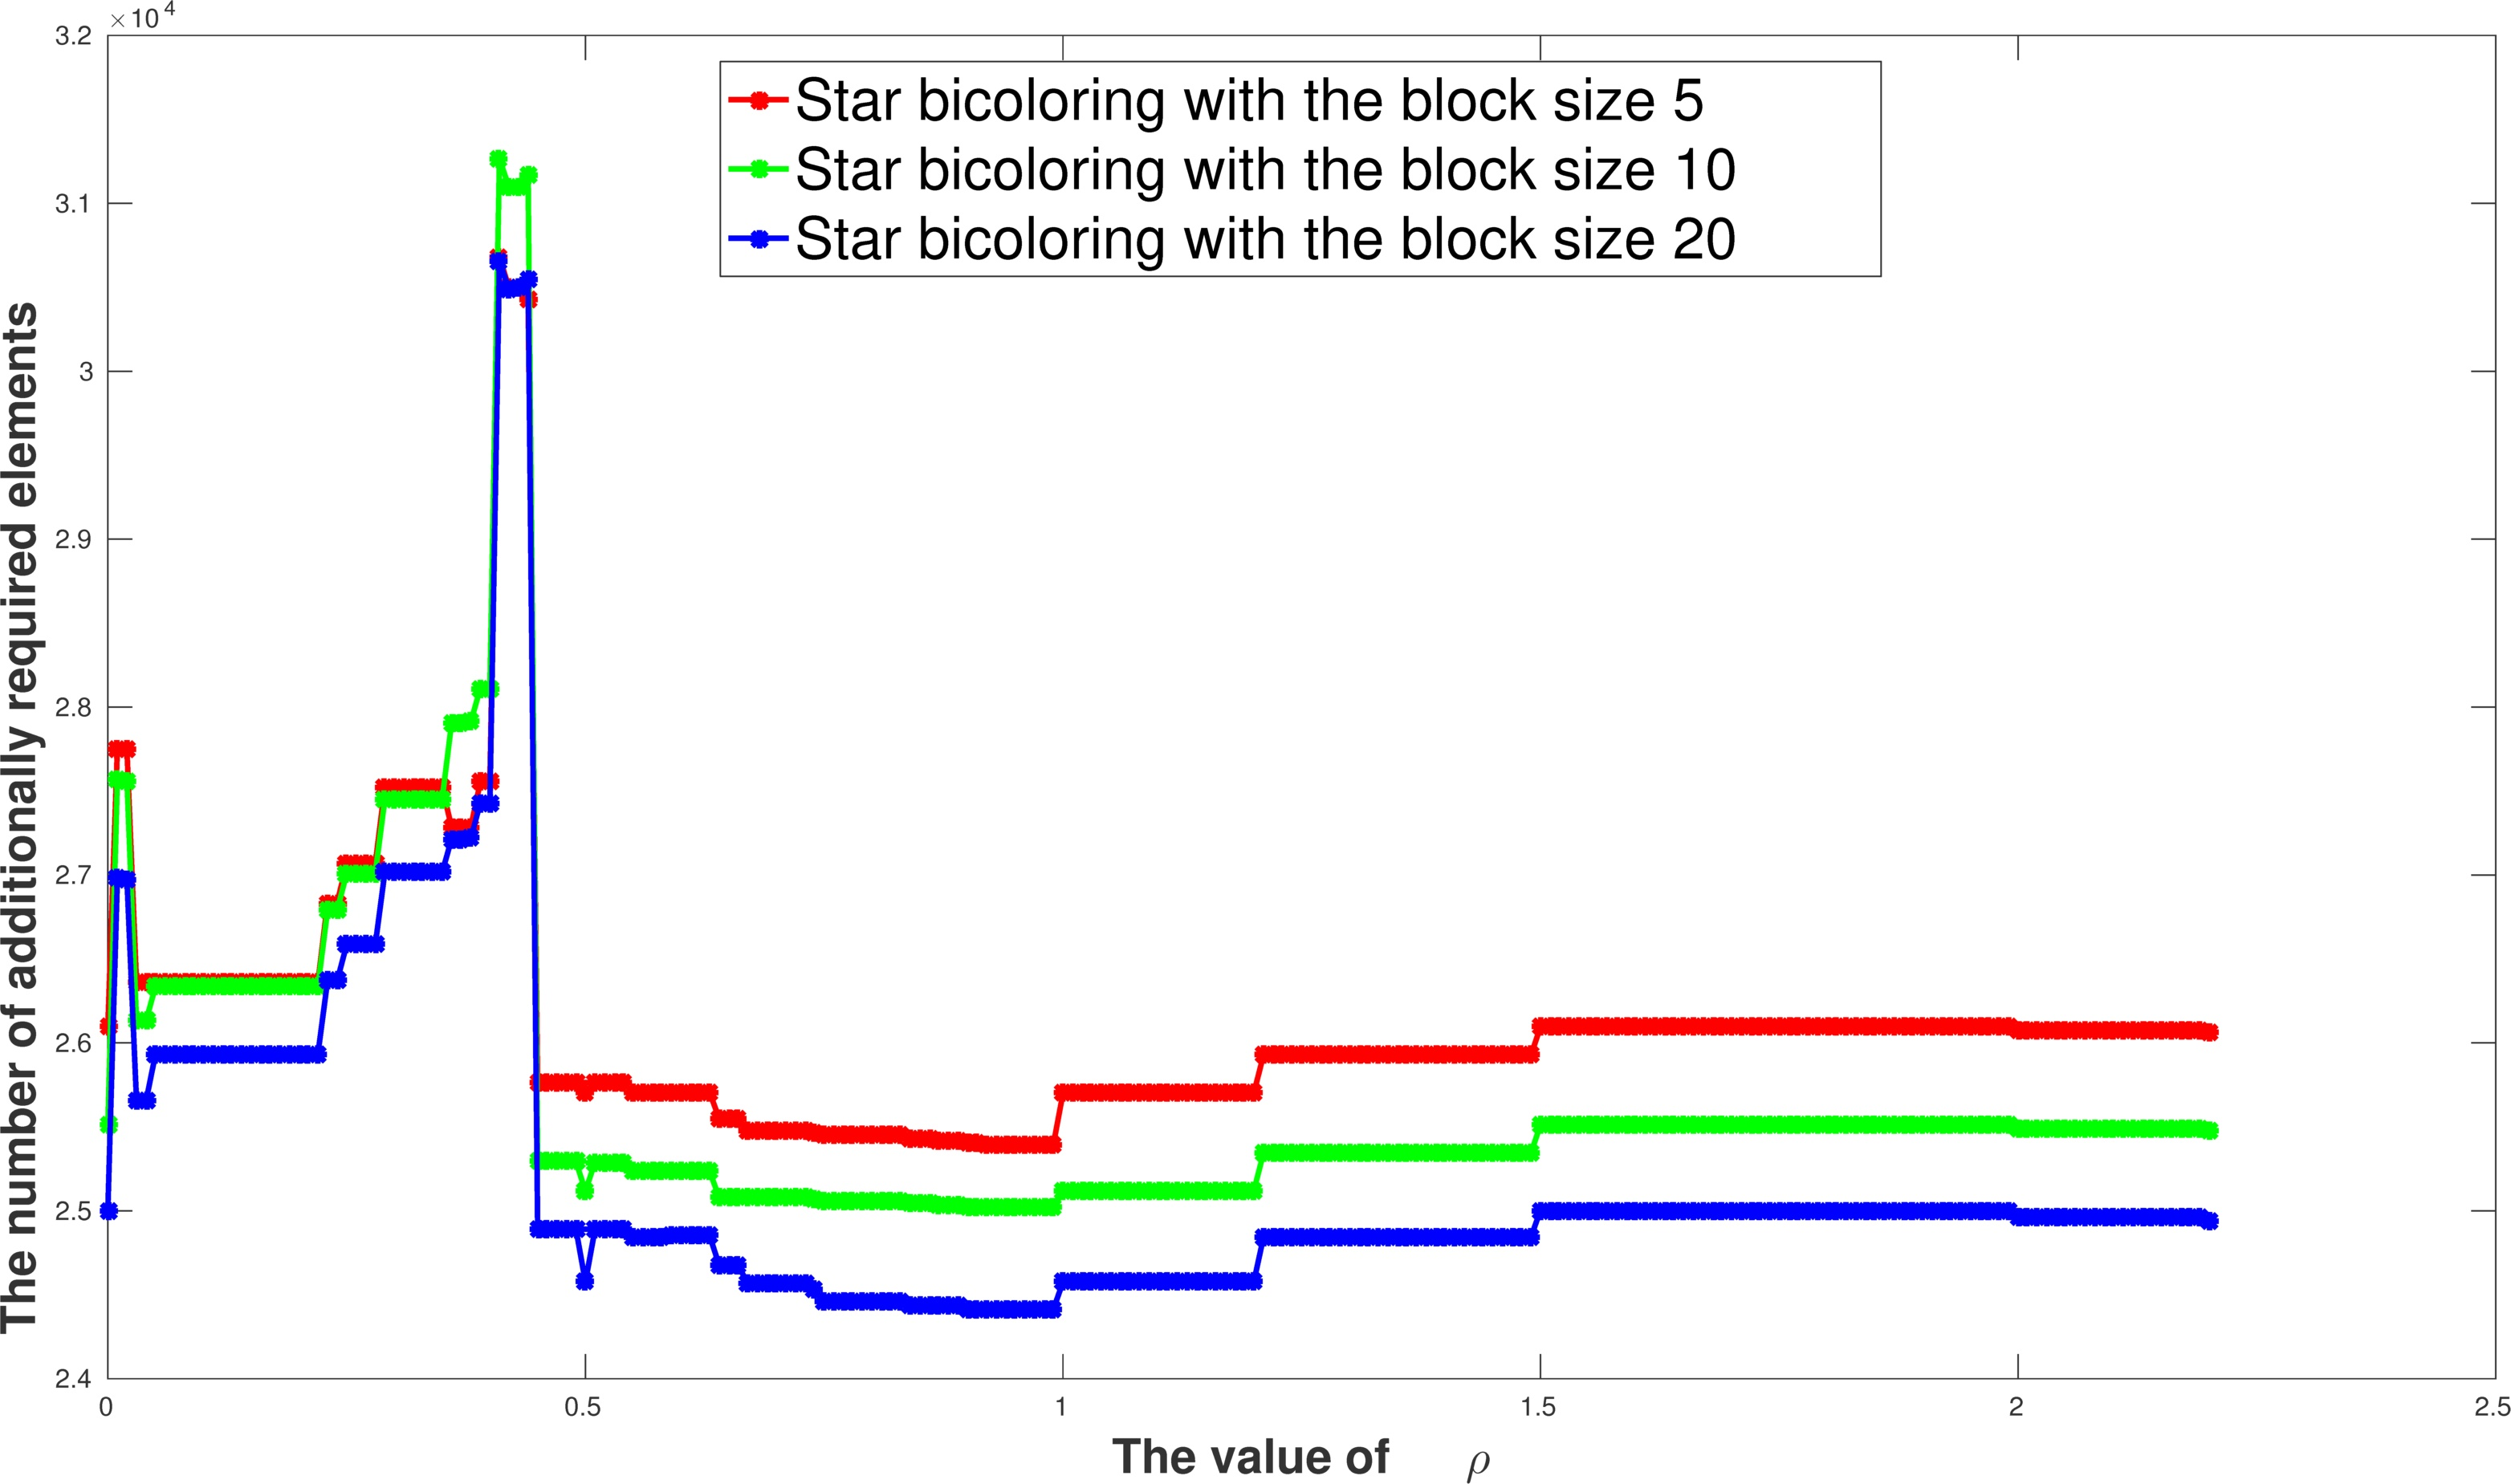
\includegraphics[width=0.9\linewidth]{rho_value_orani678}
\caption{The influence of $\rho$ is computed on the additionally required elements
for the matrix \textit{orani678} with the LFO ordering.}
\label{rho_value_orani678}
\end{figure}

Now, we introduce our new heuristic  which is a modification of \coderef{orig.star.bicoloring}.
As we said, the lines $7$ to $10$ in \coderef{orig.star.bicoloring} chooses the next vertex
which should be processed from the maximum degree vertices in a graph induces on the required edges.
\coderef{new.star.bicoloring} shows our new heuristic. Here, the parts which are the same as 
\coderef{orig.star.bicoloring} are shown by $...$.
In this algorithm, we add an extra step to this part which selects
the next vertex with the maximum determined nonrequired elements
and the minimum number of required elements.
The variable $NonReq$ switch between two modes. The first mode $NonReq=false$ selects the vertex 
based on the variable $\rho$ like \coderef{orig.star.bicoloring}. 
The second mode $NonReq=true$ selects
the next vertex with the maximum determined nonrequired elements
and the minimum number of required elements.
The other parts of algorithm is completely like \coderef{orig.star.bicoloring}.

Table~\ref{mats.pot.add.gr.vs.nreq.star} shows the numbers of potentially and additionally required elements
computed with \coderef{orig.star.bicoloring} and our new algorithm. 
We have an overall increase in both potentially and additionally required elements.

\begin{table}
\centering
\begin{tabular}{|c|c|c|c|c|}
\hline
Matrix (NAT) & \multicolumn{2}{c|}{$|R_{pot}|$} & \multicolumn{2}{c|}{$|R_{add}|$}\\\hline
{} & \coderef{orig.star.bicoloring} & \coderef{new.star.bicoloring} & \coderef{orig.star.bicoloring} & \coderef{new.star.bicoloring}\\\hline
\textit{steam1.mtx} & $64$ & $590$ & $64$ & $454$ \\\hline
\textit{steam2.mtx} & $240$ & $2352$ & $240$ & $1648$ \\\hline
\textit{nos3.mtx} & $4590$ & $4614$ & $2986$ & $3050$ \\\hline
\textit{ex7.mtx} & $35690$ & $36486$ & $28028$ & $28796$ \\\hline
\textit{ex33.mtx} & $9282$ & $11180$ & $6220$ & $7510$ \\\hline
\textit{crystm01.mtx} & $19262$ & $22716$ & $11472$ & $13978$ \\\hline
\textit{coater1.mtx} & $14402$ & $14442$ & $8296$ & $8262$ \\\hline
\textit{pesa.mtx} & $40572$ & $41460$ & $32728$ & $33956$ \\\hline
\end{tabular}
\vspace*{1cm}\newline
\begin{tabular}{|c|c|c|c|c|}
\hline
Matrix (LFO) & \multicolumn{2}{c|}{$|R_{pot}|$} & \multicolumn{2}{c|}{$|R_{add}|$}\\\hline
{} & \coderef{orig.star.bicoloring} & \coderef{new.star.bicoloring} & \coderef{orig.star.bicoloring} & \coderef{new.star.bicoloring}\\\hline
\textit{steam1.mtx} & $64$ & $802$ & $64$ & $466$ \\\hline
\textit{steam2.mtx} & $240$ & $2352$ & $240$ & $944$ \\\hline
\textit{nos3.mtx} & $4824$ & $5166$ & $3152$ & $3444$ \\\hline
\textit{ex7.mtx} & $36794$ & $37012$ & $28670$ & $28942$ \\\hline
\textit{ex33.mtx} & $11070$ & $11426$ & $7380$ & $7708$ \\\hline
\textit{crystm01.mtx} & $21420$ & $22714$ & $13012$ & $13992$ \\\hline
\textit{coater1.mtx} & $14422$ & $14496$ & $8204$ & $8350$ \\\hline
\textit{pesa.mtx} & $42758$ & $42904$ & $32272$ & $34266$ \\\hline
\end{tabular}
\vspace*{1cm}\newline
\begin{tabular}{|c|c|c|c|c|}
\hline
Matrix (SLO) & \multicolumn{2}{c|}{$|R_{pot}|$} & \multicolumn{2}{c|}{$|R_{add}|$}\\\hline
{} & \coderef{orig.star.bicoloring} & \coderef{new.star.bicoloring} & \coderef{orig.star.bicoloring} & \coderef{new.star.bicoloring}\\\hline
\textit{steam1.mtx} & $64$ & $824$ & $64$ & $616$ \\\hline
\textit{steam2.mtx} & $240$ & $2320$ & $240$ & $1616$ \\\hline
\textit{nos3.mtx} & $4314$ & $4760$ & $2784$ & $3102$ \\\hline
\textit{ex7.mtx} & $35690$ & $36450$ & $27814$ & $28568$ \\\hline
\textit{ex33.mtx} & $9728$ & $10978$ & $6468$ & $7296$ \\\hline
\textit{crystm01.mtx} & $24222$ & $27226$ & $14562$ & $16590$ \\\hline
\textit{coater1.mtx} & $14532$ & $14634$ & $8194$ & $8412$ \\\hline
\textit{pesa.mtx} & $41128$ & $42112$ & $31114$ & $33744$ \\\hline
\end{tabular}
\caption{The comparison between the number of potentially and additionally required
elements computed with \coderef{orig.star.bicoloring} and \coderef{new.star.bicoloring}.
The block size is fixed to $10$. The orderings for coloring are (Top) the natural ordering,
(Middle) LFO, and (Bottom) SLO.}
\label{mats.pot.add.gr.vs.nreq.star}
\end{table}


\begin{figure}
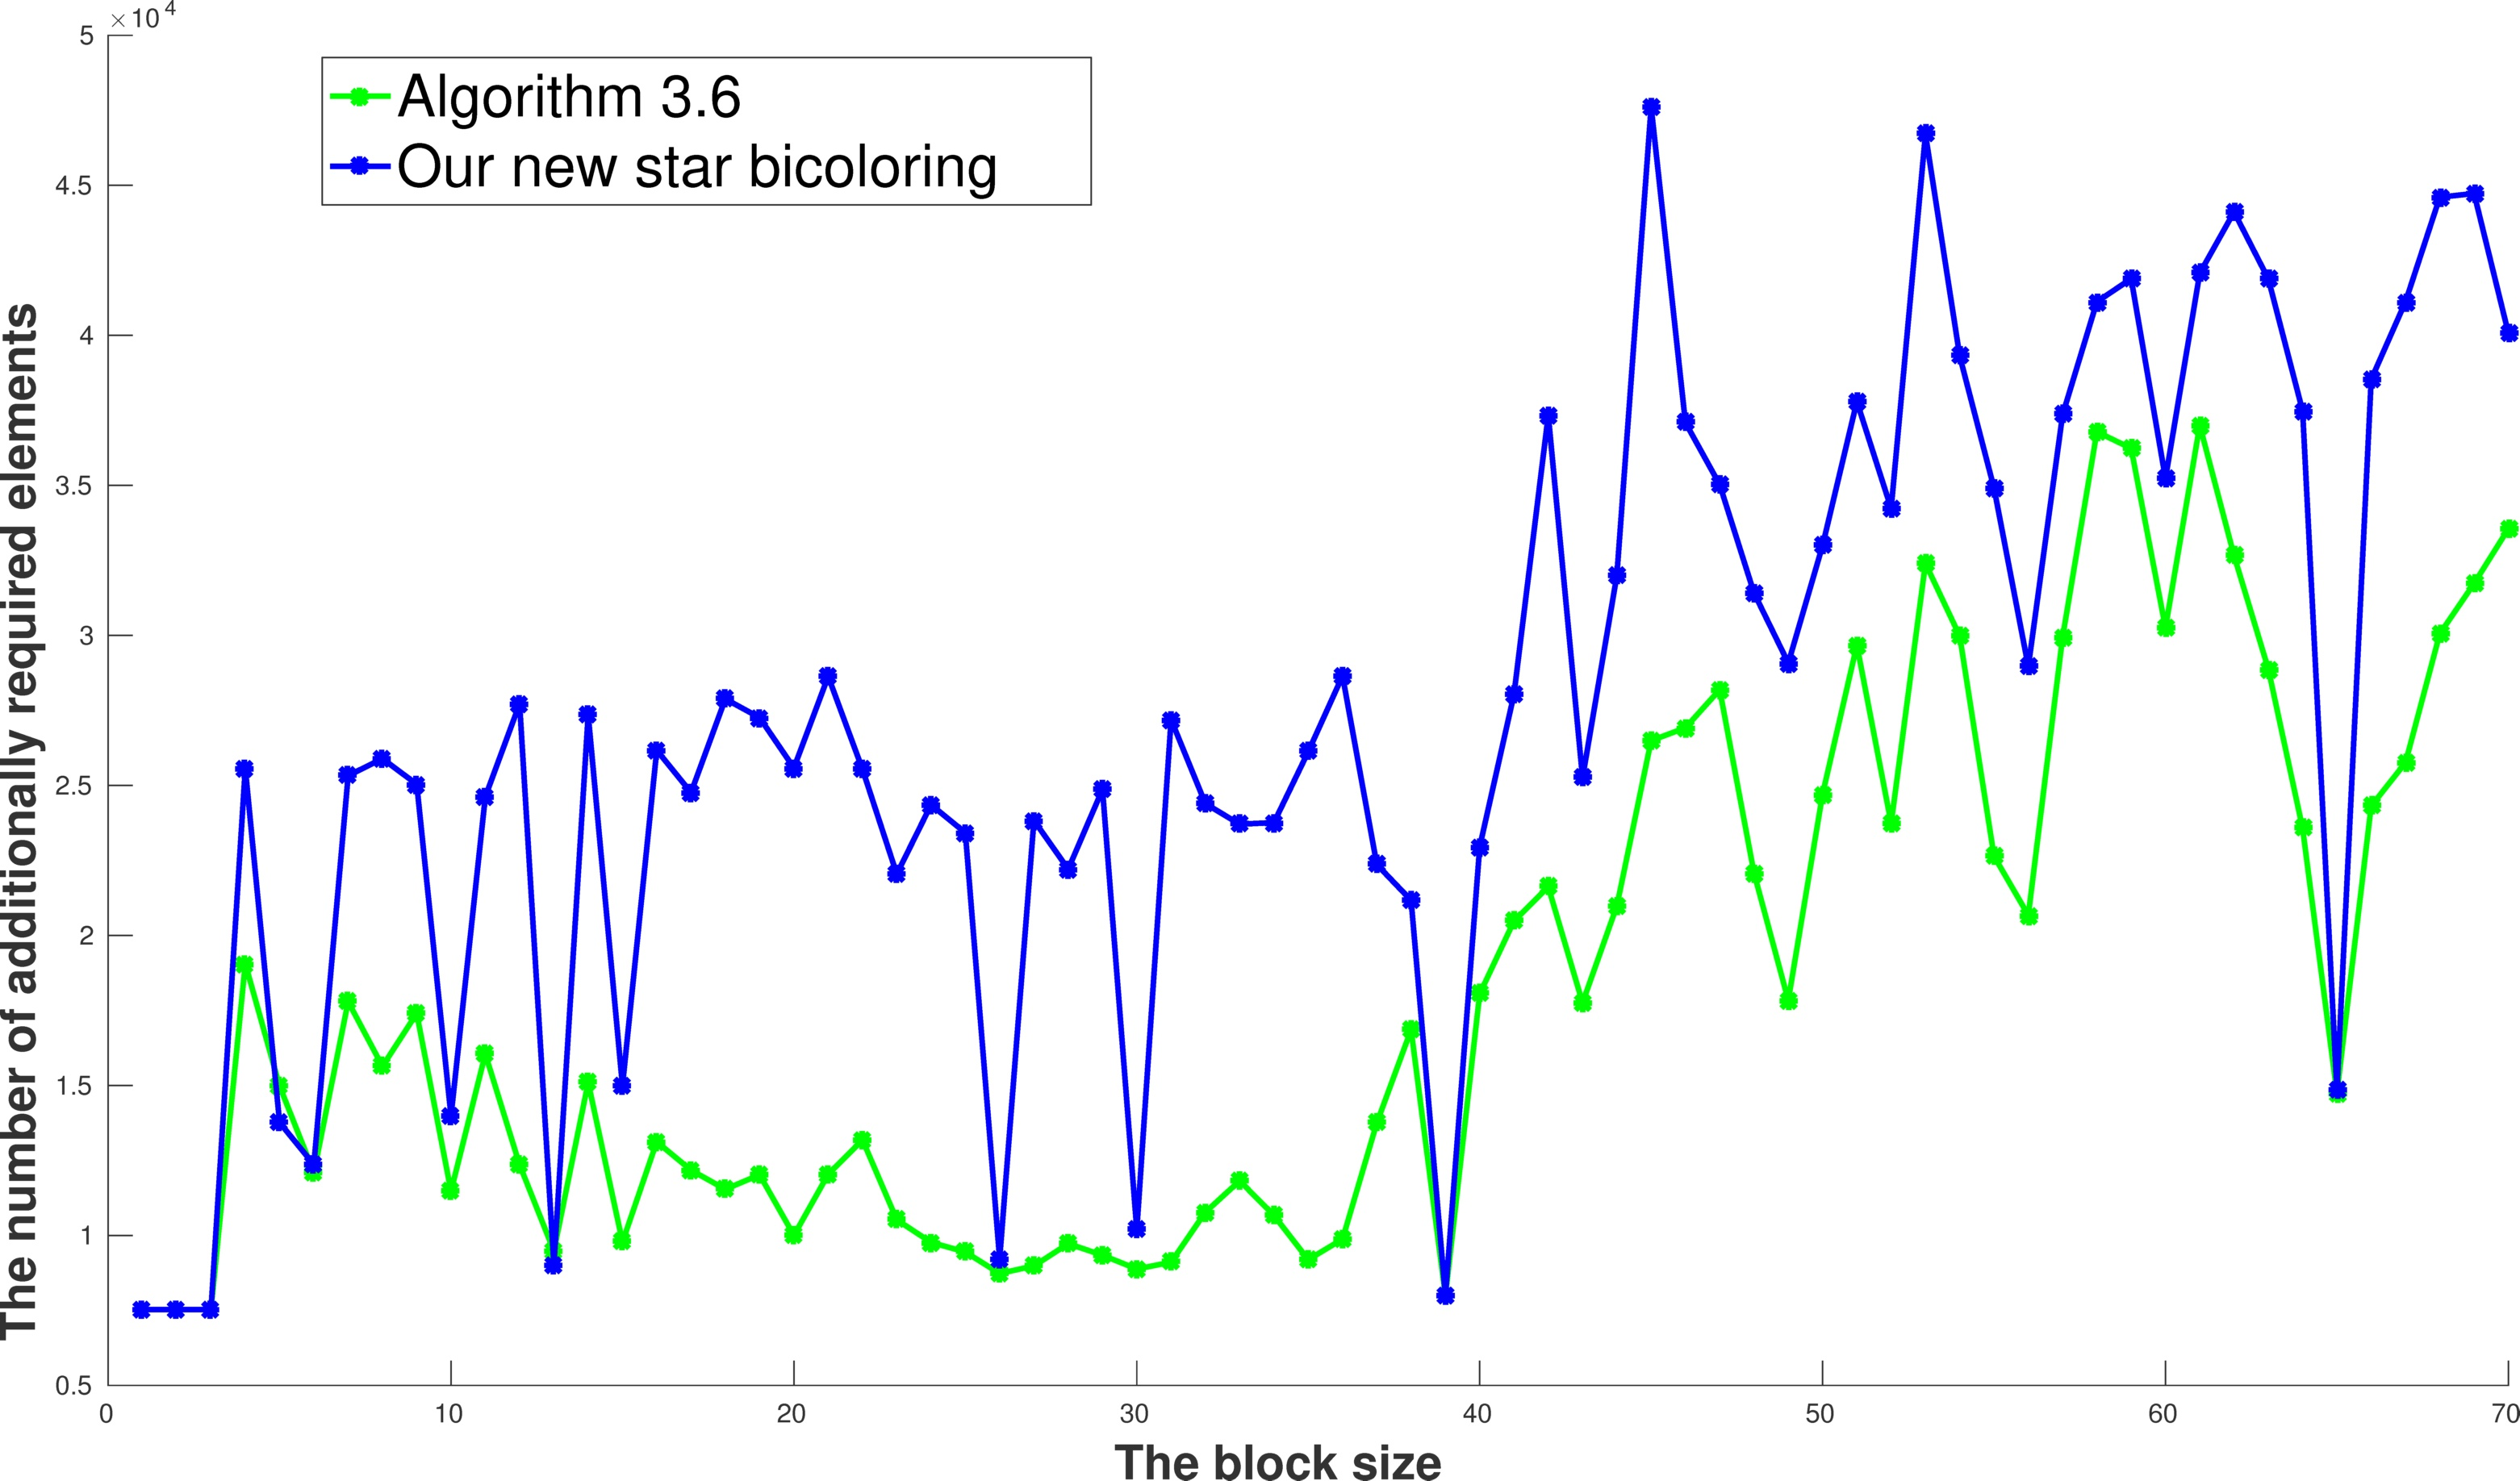
\includegraphics[width=\linewidth]{crystm01_alg36_bls_nat_adds}
\caption{The number of additionally required elements computed with
\coderef{new.star.bicoloring} compared with \coderef{orig.star.bicoloring}.
The nonsymmetric matrix \textit{$crystm01$} with the natural ordering is used here.}
\label{crystm01_alg36_bls_nat_adds}
\end{figure}



%\begin{figure}
%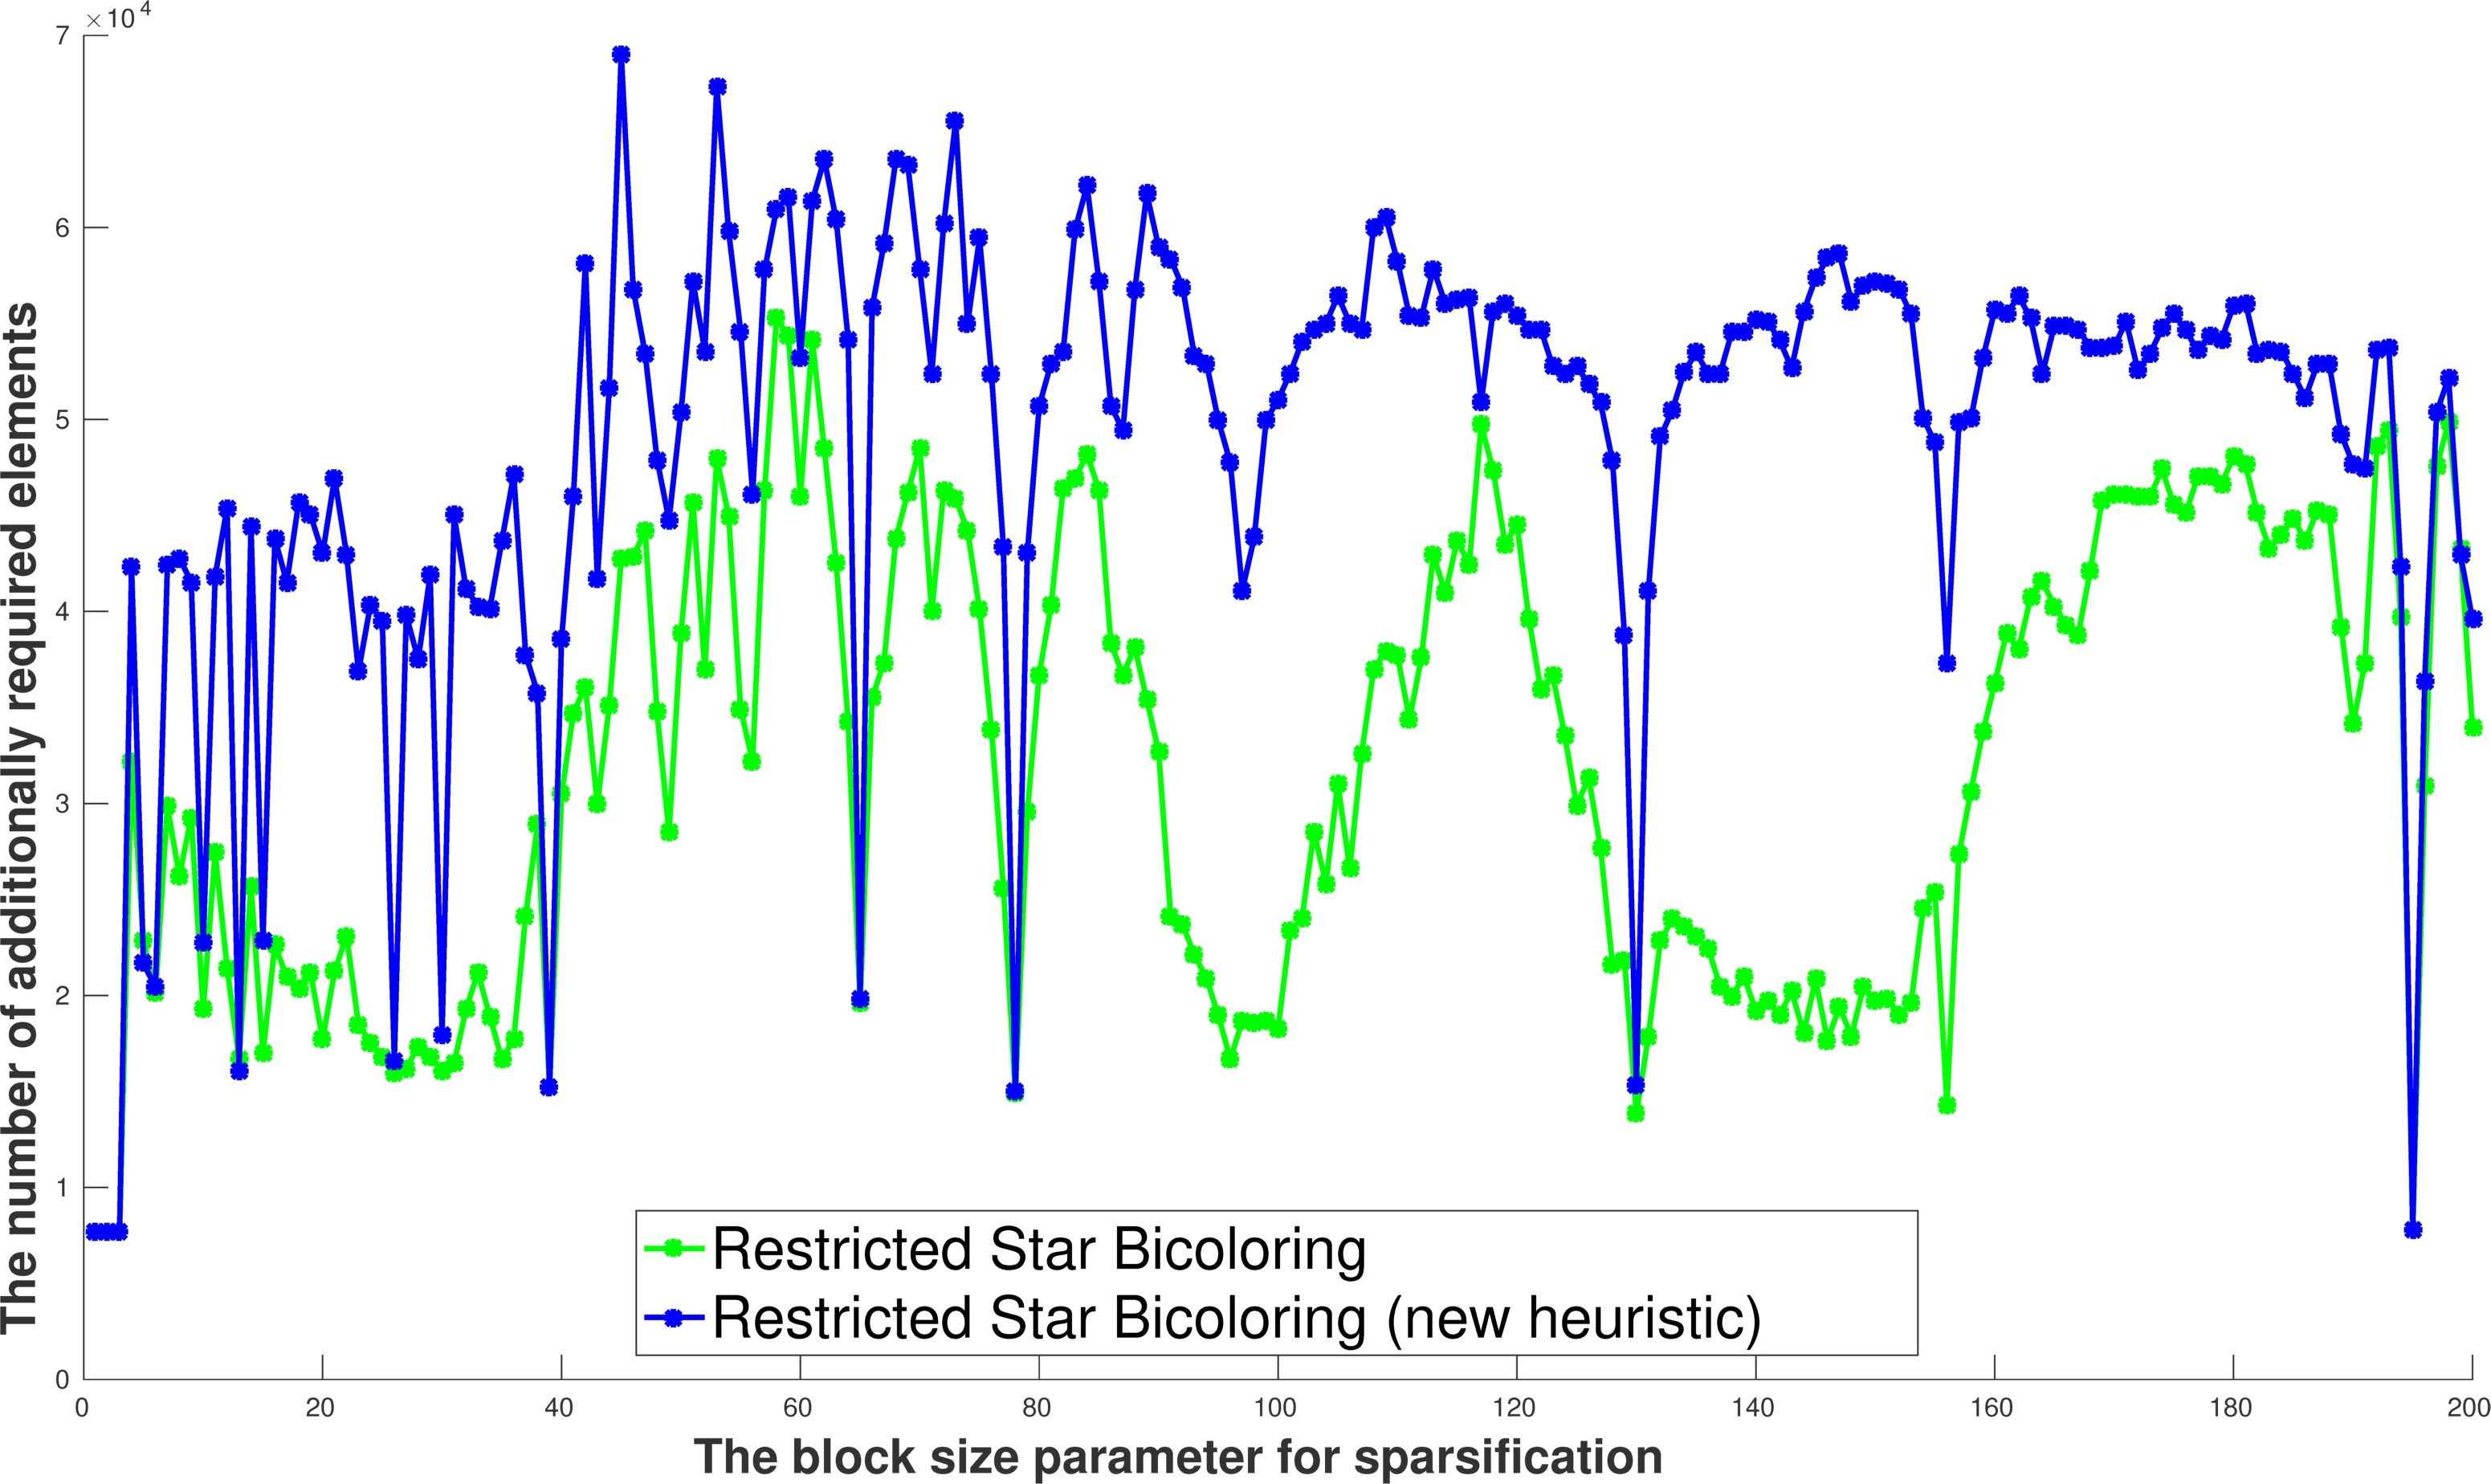
\includegraphics[width=\linewidth]{bls_adds_crystm01_old_star_vs_new}
%\caption{The number of additionally required elements computed with
%the new star bicoloring compared with the older implementation.
%The nonsymmetric matrix \textit{$crystm01$} is used here.}
%\label{bls_adds_crystm01_old_star_vs_new}
%\end{figure}

%\begin{figure}
%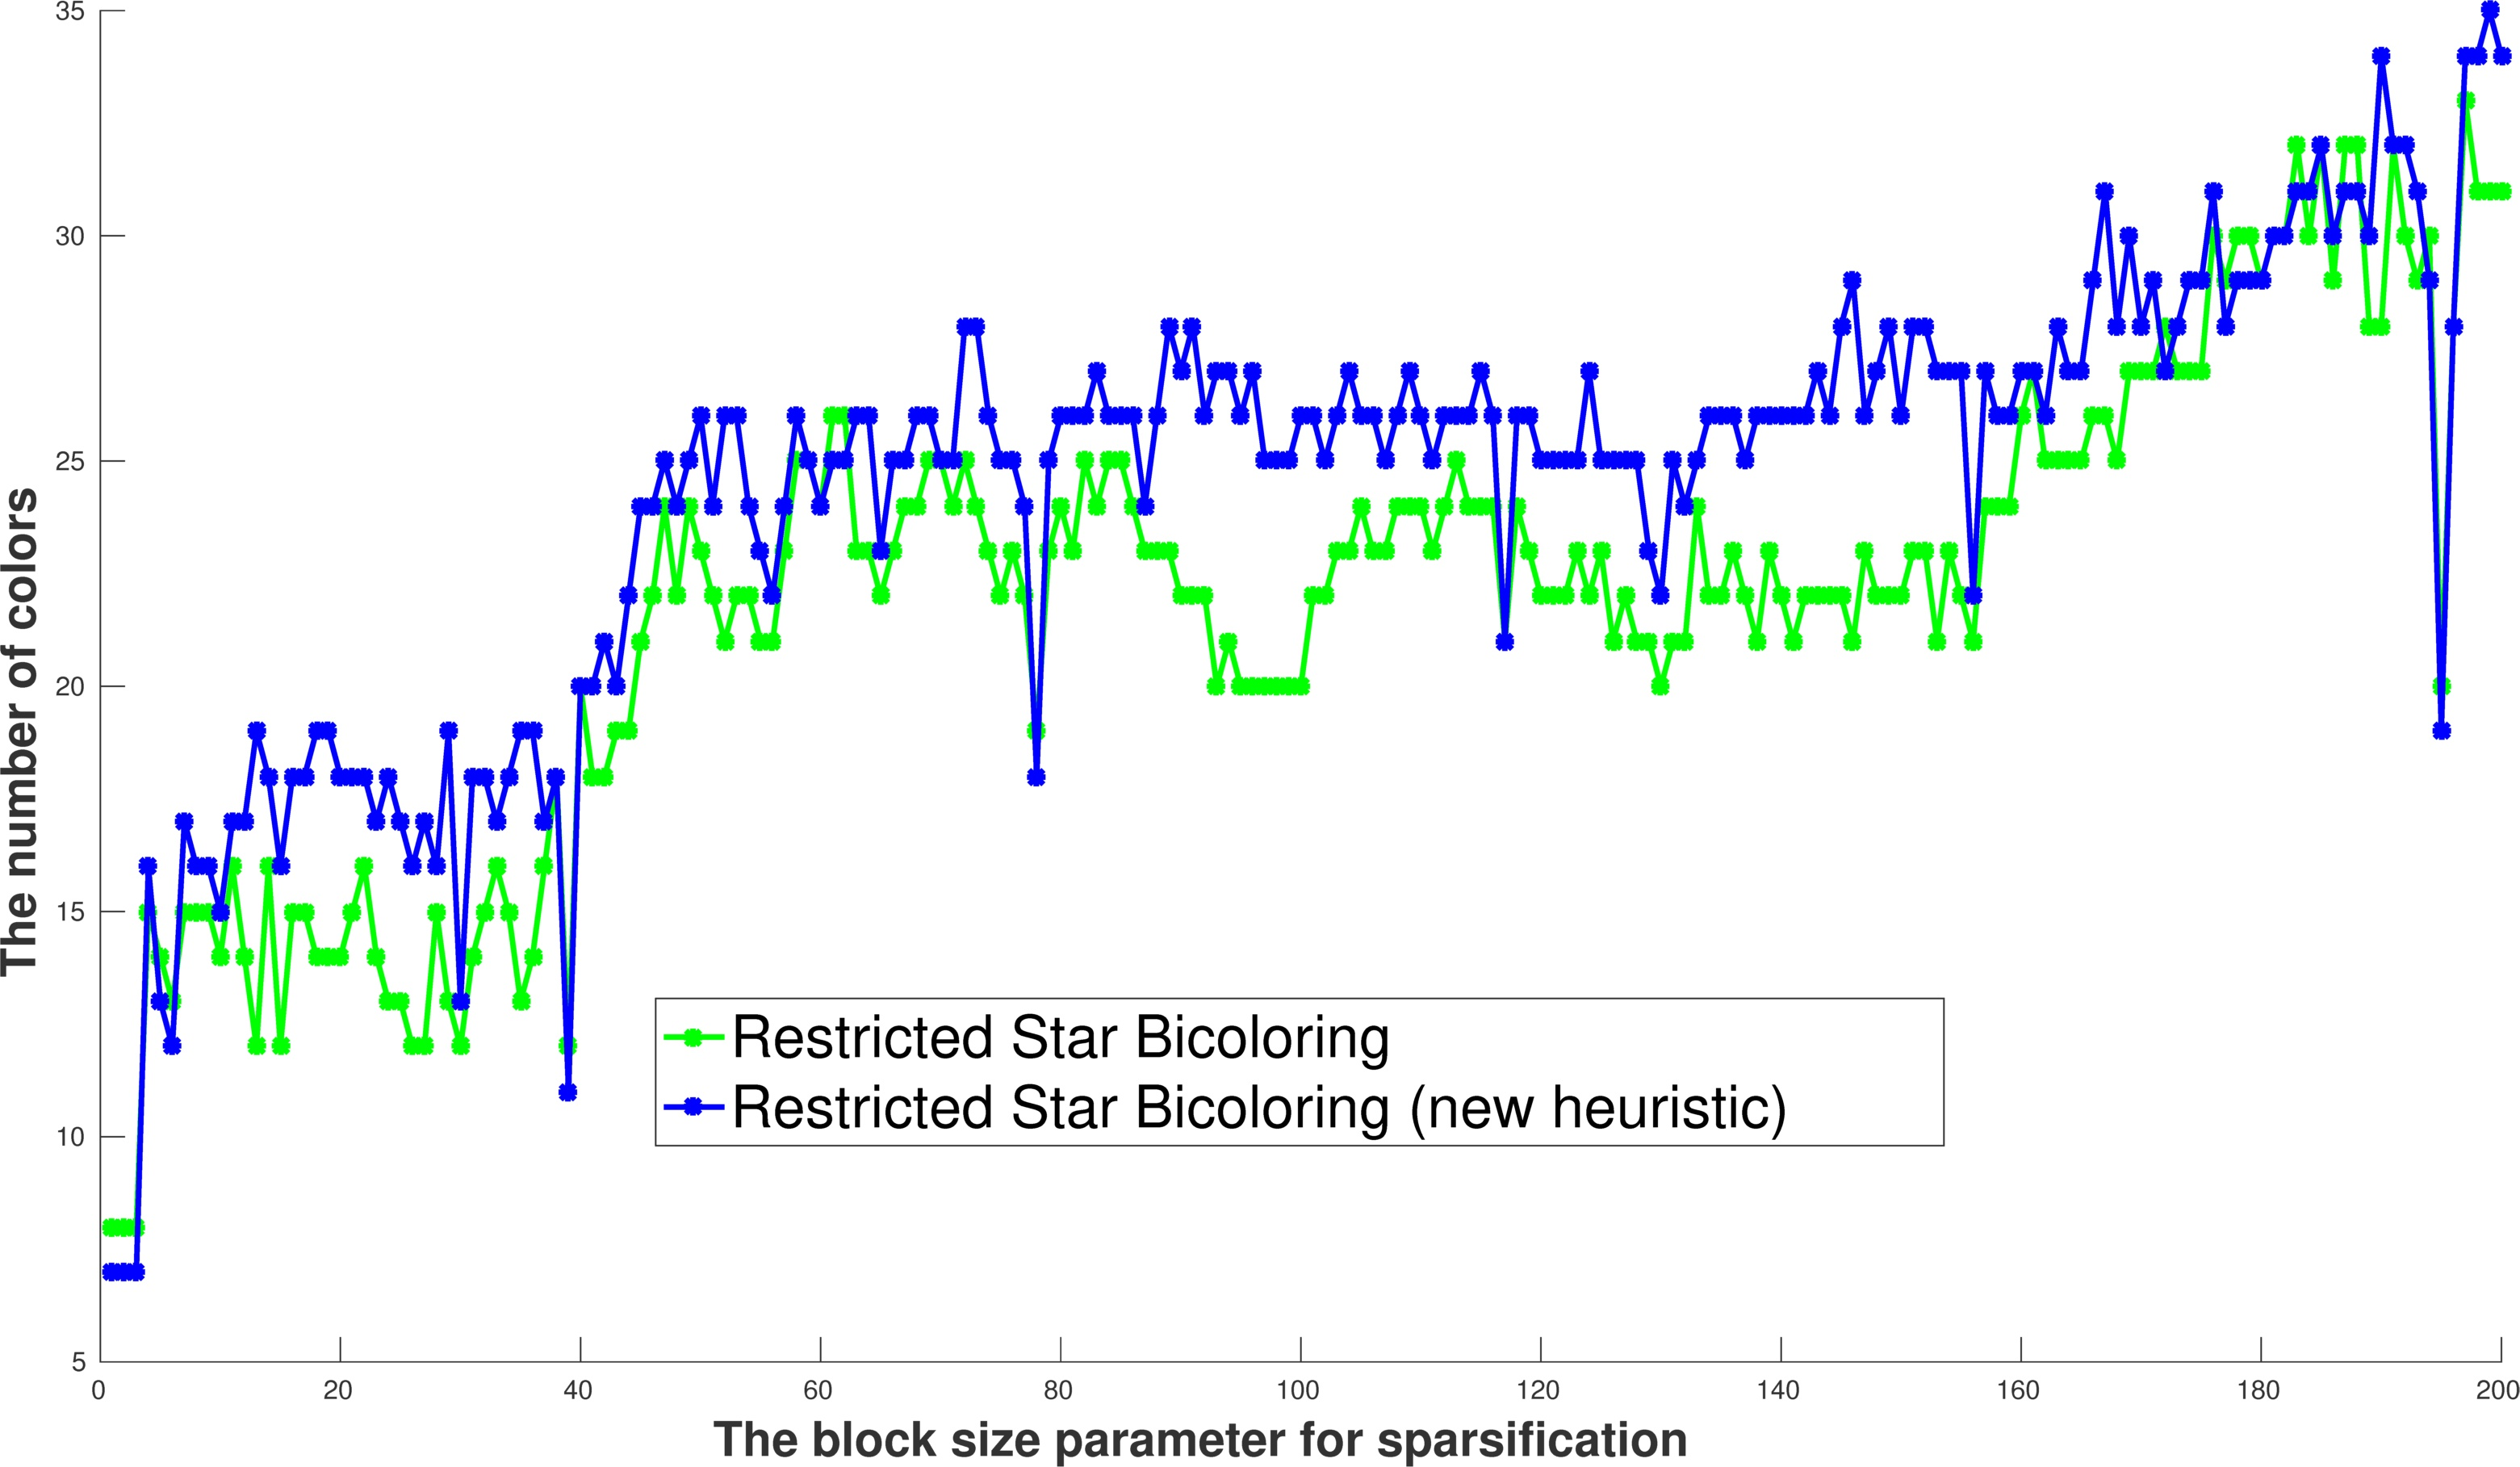
\includegraphics[width=\linewidth]{bls_cols_crystm01_old_star_vs_new}
%\caption{The number of additionally required elements computed with
%the new star bicoloring compared with the older implementation.
%The nonsymmetric matrix \textit{$crystm01$} is used here.}
%\label{bls_cols_crystm01_old_star_vs_new}
%\end{figure}
%%%%%%%%%%%%%%%%%%%%%%%%%%%%%%%%%%%%%%%%%%%%%%%%%%%%%%%%%%%%%%%%%%%%%%%%%%%%
\clearpage
\subsection{Parallelization}
\label{s.parallel}
%%%%%%%%%%%%%%%%%%%%%%%%%%%%%%%%%%%%%%%%%%%%%%%%%%%%%%%%%%%%%%%%%%%%%%%%%%%%
For a faster computation, we parallelize the proposed heuristics by OpenMP here.
There are much literature to parallelize coloring algorithms.
For example, {\c{C}}ataly{\"{u}}rek~\cite{cataly2012} introduced an OpenMP parallelized
greedy coloring which computes the same number of colors as the serial version.
However, there are two points in each iteration of the algorithm in which the threads
need to be synchronized.
Here, our focus is on another algorithm from Rokos et al~\cite{Rokos2015}
which presents an algorithm in which only a point of synchronization is
needed.
In this algorithm, the number of colors changes but it remains near 
to the number of colors in the serial version.
We adapt this parallelization to \coderef{code.greedy} and \coderef{code.new.impr2}
for the bipartite graph model as presented in \coderef{omp.greedy.bip} and \coderef{code.new.bip.omp}.
These algorithms first colors the vertices
greedily with a parallel loop and then corrects the false coloring which can happen.
\begin{figure}
\begin{lstlisting}[caption=A OpenMP parallelized version of greedy algorithm
adapted for the bipartite graph.,label=omp.greedy.bip,mathescape]
function d2_color_omp($G=(V_r\cup V_c,E)$,$E_i\subseteq E$)
  #pragma omp parallel for
  for $v\in V_c$
    $forbiddenColors[\Phi(n)] = v$
    $\Phi(v) = min \{ a>0:forbiddenColors[a]\neq v\}$
  #pragma omp barrier
  $U_0 = V_c$
  $i = 1$
  while $U_{i-1}\neq \emptyset$
    $L=\emptyset$
    #pragma omp parallel for
    for $v\in U_{i-1}$
      if $\exists u\in N_2(v,E_i), u>v: \Phi(u) = \Phi(v)$
        $forbiddenColors[\Phi(n)] = v$
        $\Phi(v) = min \{ a>0:forbiddenColors[a]\neq v\}$
    #pragma omp barrier
    $U_i = L$
    $i = i+1$
\end{lstlisting}

\begin{lstlisting}[caption=New coloring heuristic in the bipartite graph model
parallelized by OpenMP,label=code.new.bip.omp,mathescape]
function d2_color_nreq_omp($G=(V_r\cup V_c,E)$,$E_i\subseteq E$,$\alpha$)
  #pragma omp parallel for
  for $v\in V_c$ with $\Phi(v)=0$
    $forbiddenColors[0] = v$
    if $\exists n\in N_2(v,E_i): (v,n)\in E_i$
      for $n\in N_2(v,E_i)$
        if $\Phi(n) \neq 0$
          $forbiddenColors[\Phi(n)] = v$
    $\Phi(v) = min \{ a>0:forbiddenColors[a]\neq v\}$

    Determine an indepentent set $I_v$ containing $v$
    if $I_v-\{v\}\neq\emptyset$
      $maxs = \argmax_{x\in I_v - \{v\}} \nreq_v (x)$
      $mins = \argmin_{x\in maxs} \req(x)$ 
      for $i\in\{0,1,...,\min (\alpha - 1, size(mins))\}$
        $\Phi(mins[i]) = \Phi(v)$

  #pragma omp barrier
  $U_0 = V$
  $i = 1$
  while $U_{i-1}\neq \emptyset$
    $L=\emptyset$
    #pragma omp parallel for
    for $v\in U_{i-1}$
      if $\exists u\in N_2(v,E_i), u>v: \Phi(u) = \Phi(v)$
        $forbiddenColors[\Phi(n)] = v$
        $\Phi(v) = min \{ a>0:forbiddenColors[a]\neq v\}$

    #pragma omp barrier
    $U_i = L$
    $i = i+1$
\end{lstlisting}
\end{figure}

We color the bipartite graph interpreted from the matrix \textit{Cavity16}
from the sparse matrix collection of the University of Florida.
The timing results are all from the computation carried on an Intel Core i5 with 8 Gb RAM.
Table~\ref{omp.res} shows the results of these computations.
Here, we change the number of threads from $1$ to $10$ shown in the first column.
The second column shows the computation time in milliseconds. The third column
is also the number of colors which changes based on the number of colors.
Table~\ref{omp.res}(Left) shows the results of computation of \coderef{omp.greedy.bip}
and Table~\ref{omp.res}(Right) for \coderef{code.new.bip.omp}.
Also \figref{speedups} (Left) and \figref{speedups} (Right) visualize the speedup
based on the number of threads.
\begin{figure}
\begin{tabular}{|c|c|c|}
\hline
Threads & Time & Colors \\\hline
1 & 42.8745 & 47 \\\hline
2 & 33.9665 & 47 \\\hline
3 & 25.2741 & 48 \\\hline
4 & 20.6863 & 48 \\\hline
5 & 21.4943 & 47 \\\hline
6 & 20.1796 & 50 \\\hline
7 & 17.9640 & 49 \\\hline
8 & 16.1068 & 52 \\\hline
9 & 15.4174 & 47 \\\hline
10 & 16.1545 & 47 \\\hline
\end{tabular}\hfill
\begin{tabular}{|c|c|c|}
\hline
Threads & Time & Colors \\\hline
1 & 96.795 & 48 \\\hline
2 & 75.744 & 47 \\\hline
3 & 55.605 & 49 \\\hline
4 & 49.335 & 49 \\\hline
5 & 49.360 & 47 \\\hline
6 & 49.365 & 51 \\\hline
7 & 45.342 & 47 \\\hline
8 & 43.254 & 51 \\\hline
9 & 40.742 & 48 \\\hline
10 & 39.416 & 47 \\\hline
\end{tabular}
\caption{
(Left) The results of computation of greedy coloring parallelized by OpenMP.
(Right) The results of computation of new heuristics parallelized by OpenMP}
\label{omp.res}
\end{figure}

\begin{figure}
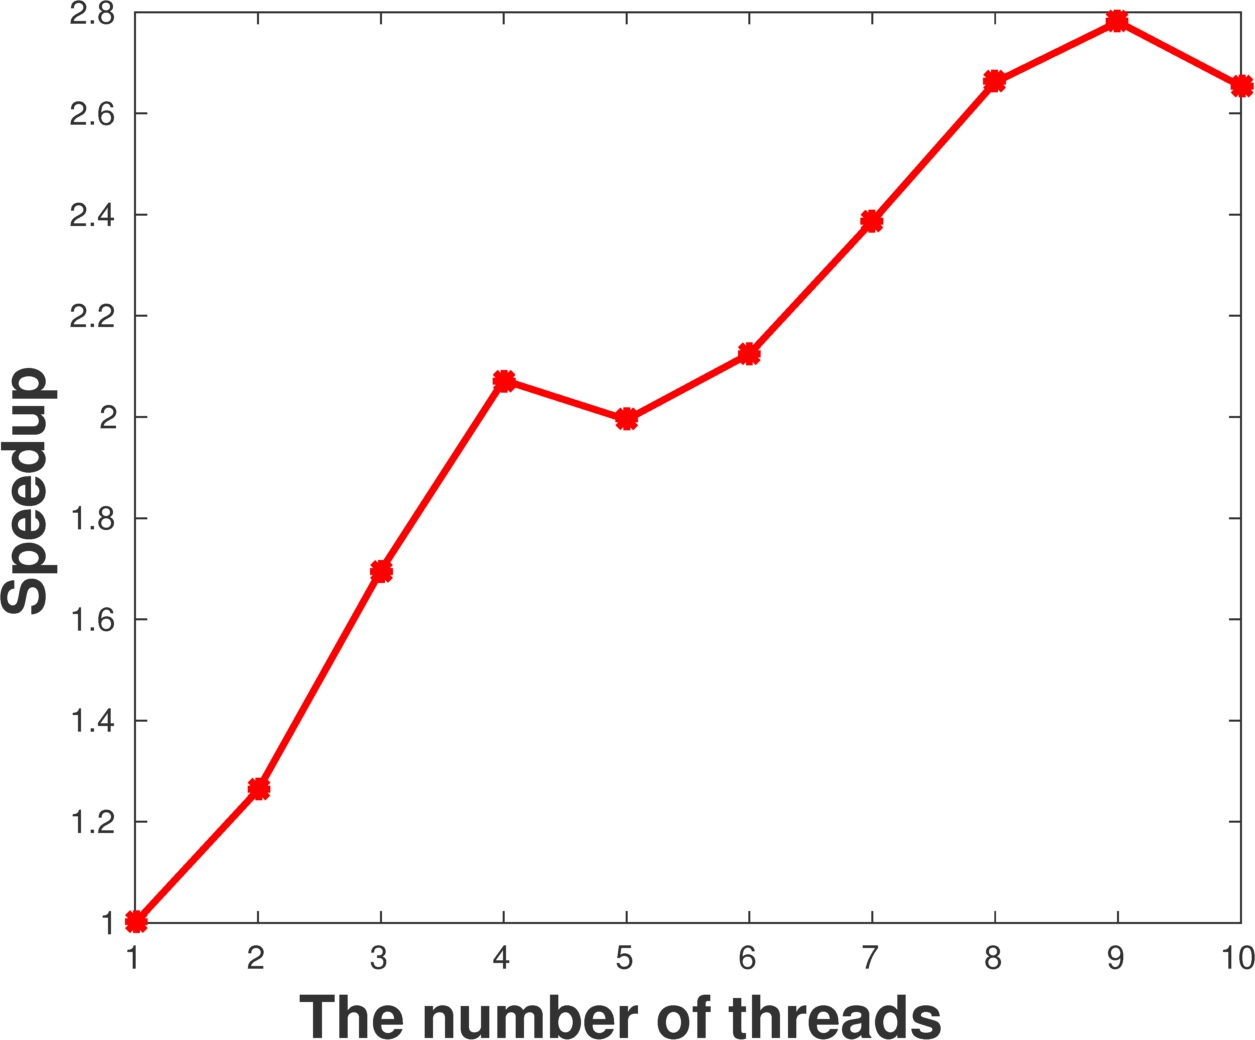
\includegraphics[width=0.44\linewidth]{ths_spd.jpg}\hfill
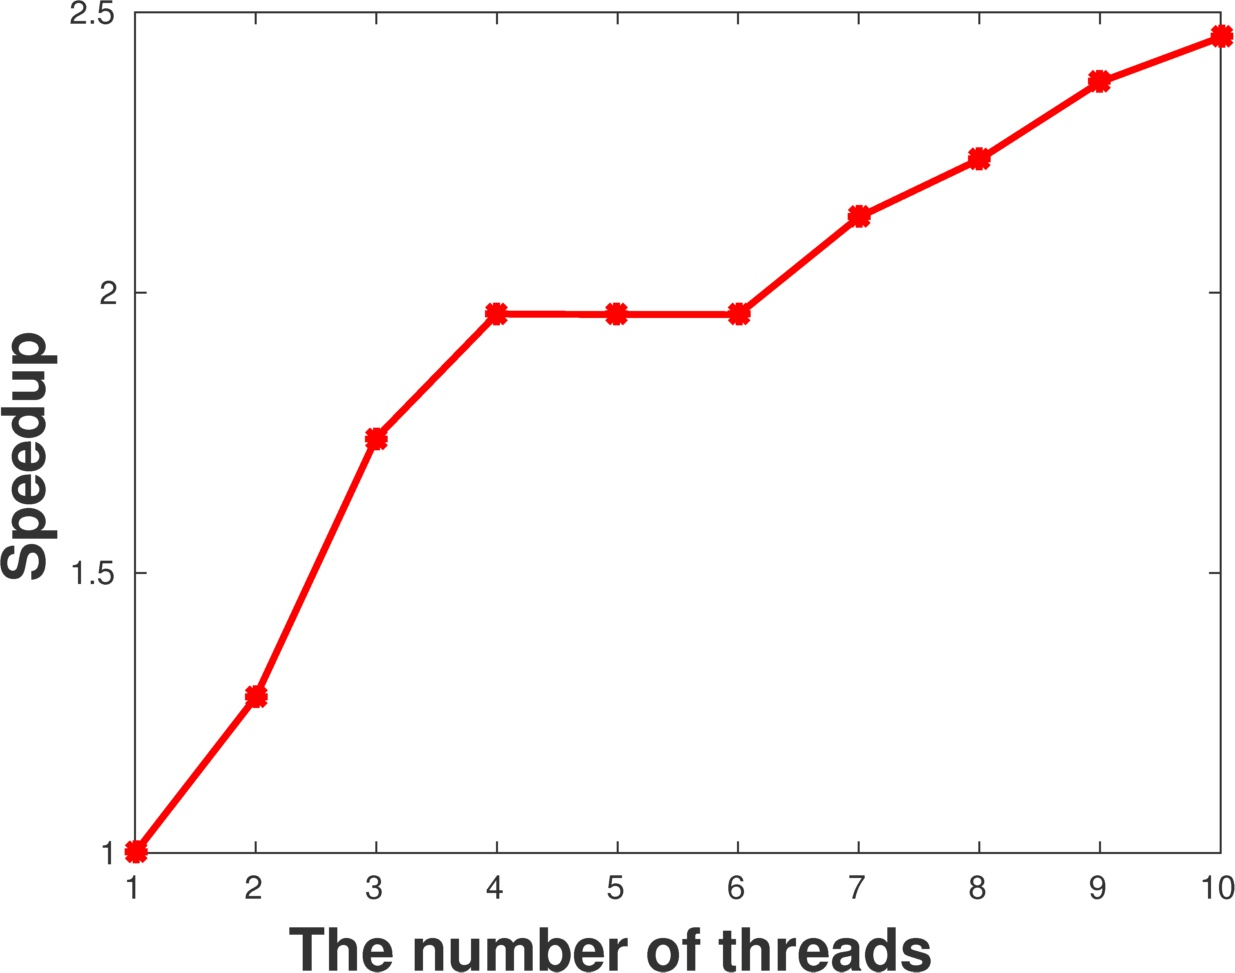
\includegraphics[width=0.47\linewidth]{ths_spd2.jpg}
\caption{
(Left) Speedup for the computation of greedy coloring in bipartite graph model parallelized by OpenMP.
(Right)Speedup for the computation of new coloring heuristic in bipartite graph model parallelized by OpenMP.
}
\label{speedups}
\end{figure}

This idea can be applied to the new heuristic for star bicoloring which is a potential future work.
Apart from the parallelization of coloring, the block diagonal sparsification makes a suitable
matrix for parallelization. It is well known the fill-ins are generated only in the nonzero blocks in such matrices. This observation gives a direct idea of parallelization in which each process
works on each block. We do not go into details since it is already discussed in previous literature like~\cite{parblockilu}. However, it does not mean that the same idea can be applied in computation of
additionally required elements since those elements are outside the blocks.

%\cite{mpi_greedy_coloring}
%%%%%%%%%%%%%%%%%%%%%%%%%%%%%%%%%%%%%%%%%%%%%%%%%%%%%%%%%%%%%%%%%%%%%%%%%%%%%%%%%%%%%%%%
\clearpage
\section{Maximizing the set of additionally required elements}
\label{s.max.add.req}
%%%%%%%%%%%%%%%%%%%%%%%%%%%%%%%%%%%%%%%%%%%%%%%%%%%%%%%%%%%%%%%%%%%%%%%%%%%%%%%%%%%%%%%%%
In \secref{s.max.pot.req}, we consider algorithms to increase the potentially required elements
which increases the number of additionally required elements presumably.
Here, we suggest a heuristic to predict if a nonrequired element would be an
additionally required element. 
For this purpose, we use the bipartite graph model for ILU preconditioning
presented in \secref{ss.comb.precond} and the its adapted concept of fill path in 
\defref{d.fill.path.bipartite}. Given a nonrequired element (an edge of bipartite graph),
the idea is to check if the addition of this edge would generate any new fill-in.
If the fill level of SILU is $l$, we list all fill paths of length $l$ passing this nonrequired edge
in the set $L$. Each fill path in the set $L$ which all its edges except the given nonrequired edge
are required edges would later generate a fill-in. So, it is more efficient not to add the
nonrequired edge in this case.

As we discussed, for a fixed ordering of vertices,
a fill path from the vertex $v_i$ to $v_j$ is a path $v_i,...,v_k,...,v_j$
in which all intermediate vertices has smaller indices than $i$ and $k$.
Given a nonrequired edge $t=(r_i,c_j)$, we define the set of all fill paths starting
from $c_i$ passing the edge $t$ with the size of $k$ as
$pr_k^t = \{\{ r_i,c_j,...,c_a\},...,\{ r_i,c_j,...,c_b\}\}$.
Equivalently, we define the set of all fill paths ending to the vertex $c_j$
passing the edge $t$ with the size of $k$ as
$pl_k^t = \{ \{c_d,...,r_i,c_j\},..., \{c_e,...,r_i,c_j\}\}$.
With these definitions, \coderef{code.new.d2.add.fp} is a coloring heuristic
for distance-$2$ coloring which checks if a determined nonzero element can be an
additionally required element. 
\begin{figure}
\begin{lstlisting}[caption=New coloring heuristic for distance-$2$ coloring
predicting if a determined nonrequired elements can be an additionally required element.,
label=code.new.d2.add.fp,mathescape]
function d2_color_fillpath($G=(V_r\cup V_c,E)$,$E_i\subset E$, $k$)
  for $v\in V_c$
    $\Phi(v)=-1$
    $forbiddenColors[v] = 0$

  for $v\in V_c$ with $\Phi(v)=0$
    $forbiddenColors[0] = v$
    if $\exists n\in N_2(v,E_i): (v,n)\in E_i$
      for $n\in N_2(v,E_i)$
        if $\Phi(n) \neq 0$
          $forbiddenColors[\Phi(n)] = v$
    $\Phi(v) = min \{ a>0:forbiddenColors[a]\neq v\}$

    Determine an indepentent set $I_v$ containing $v$
    if $I_v-\{v\}\neq\emptyset$
      $maxs = \argmax_{x\in I_v - \{v\}} \nreq_v (x)$
      for $t\in \{(v,u): u\in maxs\}$
        if $pr_k^t = \emptyset$ and $pl_k^t = \emptyset$
          $\Phi(v) = min \{ a>0:forbiddenColors[a]\neq v\}$

  return $\Phi$
\end{lstlisting}
\end{figure}
Table~\ref{mats.add.gr.vs.nreq.vs.fillpath} shows the comparison between the number of additionally required elements
which is computed by three algorithms \coderef{code.greedy},
 \coderef{code.new.impr1}, and \coderef{code.new.d2.add.fp}. We generated more additionally required elements
by considering this new method.
\begin{table}
\centering
\begin{tabular}{|c|c|c|c|c|}
\hline
Name & \coderef{code.greedy}& \coderef{code.new.impr1} & \coderef{code.new.d2.add.fp}\\\hline
\textit{steam1} & $64$ & $630$ & $450$ \\\hline
\textit{steam2} & $240$ & $1400$ & $1466$ \\\hline
\textit{nos3} & $1106$ & $4136$ & $4145$\\\hline
\textit{ex33} & $4920$ & $5470$ & $5534$\\\hline
\textit{crystm01} & $10338$ & $28318$ & $29934$\\\hline
\end{tabular}
\caption{The comparison between the number of additionally required
elements computed by different algorithms. The block size is fixed to $10$.}
\label{mats.add.gr.vs.nreq.vs.fillpath}
\end{table}

\begin{table}
\centering
\begin{tabular}{|c|c|c|c|c|}
\hline
Matrix (NAT) & \multicolumn{2}{c|}{$|R_{pot}|$} & \multicolumn{2}{c|}{$|R_{add}|$}\\\hline
{} & \coderef{code.greedy} & \coderef{code.new.d2.nreq} & \coderef{code.greedy} & \coderef{code.new.d2.nreq}\\\hline
\textit{steam1.mtx} & $64$ & $786$ & $64$ & $630$ \\\hline
\textit{steam2.mtx} & $240$ & $1880$ & $240$ & $1400$ \\\hline
\textit{nos3.mtx} & $1638$ & $6756$ & $1106$ & $4296$ \\\hline
\textit{crystm01.mtx} & $17822$ & $47556$ & $10388$ & $28318$ \\\hline
\textit{ex7.mtx} & $38554$ & $34954$ & $29174$ & $25054$ \\\hline
\textit{ex33.mtx} & $7408$ & $8934$ & $4920$ & $5572$ \\\hline
\textit{coater1.mtx} & $11722$ & $11558$ & $7684$ & $7448$ \\\hline
\textit{pesa.mtx} & $36972$ & $41154$ & $31010$ & $33094$ \\\hline
\end{tabular}
\vspace*{1cm}\newline
\begin{tabular}{|c|c|c|c|c|}
\hline
Matrix (LFO) & \multicolumn{2}{c|}{$|R_{pot}|$} & \multicolumn{2}{c|}{$|R_{add}|$}\\\hline
{} & \coderef{code.greedy} & \coderef{code.new.d2.nreq} & \coderef{code.greedy} & \coderef{code.new.d2.nreq}\\\hline
\textit{steam1.mtx} & $64$ & $1048$ & $64$ & $666$ \\\hline
\textit{steam2.mtx} & $240$ & $2624$ & $240$ & $1248$ \\\hline
\textit{nos3.mtx} & $1880$ & $6882$ & $1246$ & $4442$ \\\hline
\textit{crystm01.mtx} & $20326$ & $36634$ & $12256$ & $21194$ \\\hline
\textit{ex7.mtx} & $37080$ & $33426$ & $28904$ & $24060$ \\\hline
\textit{ex33.mtx} & $10574$ & $10564$ & $7170$ & $6888$ \\\hline
\textit{coater1.mtx} & $11312$ & $11512$ & $7410$ & $7536$ \\\hline
\textit{pesa.mtx} & $42490$ & $41676$ & $31790$ & $31884$ \\\hline
\end{tabular}
\vspace*{1cm}\newline
\begin{tabular}{|c|c|c|c|c|}
\hline
Matrix (SLO) & \multicolumn{2}{c|}{$|R_{pot}|$} & \multicolumn{2}{c|}{$|R_{add}|$}\\\hline
{} & \coderef{code.greedy} & \coderef{code.new.d2.nreq} & \coderef{code.greedy} & \coderef{code.new.d2.nreq}\\\hline
\textit{steam1.mtx} & $64$ & $1294$ & $64$ & $754$ \\\hline
\textit{steam2.mtx} & $240$ & $3192$ & $240$ & $1912$ \\\hline
\textit{nos3.mtx} & $1682$ & $6772$ & $1132$ & $4382$ \\\hline
\textit{crystm01.mtx} & $24478$ & $45166$ & $14252$ & $26782$ \\\hline
\textit{ex7.mtx} & $36486$ & $34448$ & $27044$ & $24164$ \\\hline
\textit{ex33.mtx} & $8024$ & $10754$ & $5186$ & $7138$ \\\hline
\textit{coater1.mtx} & $10476$ & $11702$ & $7004$ & $7878$ \\\hline
\textit{pesa.mtx} & $39606$ & $44624$ & $29034$ & $34044$ \\\hline
\end{tabular}
\caption{The comparison between the number of potentially and additionally required
elements computed with \coderef{code.new.d2.nreq} and \coderef{code.greedy}.
The block size is fixed to $10$. The orderings for coloring are (Top) the natural ordering,
(Middle) LFO, and (Bottom) SLO.}
\label{mats.pot.add.gr.vs.nreq}
\end{table}
%%%%%%%%%%%%%%%%%%%%%%%%%%%%%%%%%%%%%%%%%%%%%%%%%%%%%%%%%%%%%%%%%%%%%%%%%%%%%%%%%%%%%%%%%%%%%%
\section{Application in geoscience}
\label{s.application}
%%%%%%%%%%%%%%%%%%%%%%%%%%%%%%%%%%%%%%%%%%%%%%%%%%%%%%%%%%%%%%%%%%%%%%%%%%%%%%%%%%%%%%%%%%%%%%
Here, we apply our new heuristics to the carbon sequestration example from geoscience.
The geophysics group of RWTH Aachen simulates the injection of CO\textsubscript{2}
in a reservoir by a two-phase flow model in porous media. These two phases are a wetting
and non-wetting phase like water and gas. A 2D two-phase flow can be formulated as
a system of coupled non-linear partial differential equations in which the boundary conditions
are Dirichlet and Neumann. Integrating the time with the implicit Euler method
based on~\cite{Lulfesmann2012Fap}, the following system of non-linear equations are resulted,
$$F(u)=0 \, \text{ with } \, u = \binom{p_w}{S_n} \in \R^{2MN} \, \text{ and } \, F = \binom{F_1}{F_2} \in \R^{2MN},$$
where the variable $p_w \in \R^{MN}$ is the pressure for the wetting phase and $S_n \in \R^{MN}$ is the non-wetting saturation. The Newton's method solves this system of equations.
Hence, the $2MN \times 2MN$ Jacobian matrix $A$ is determined with a transformed version of the original function $F$ (The AD tool \mbox{ADiMat}~\cite{Bischof2005AML} transforms $F$),
$$
A =
\left({\begin{array}{l|l}
	\displaystyle \frac{\partial F_1}{\partial p_w} & \displaystyle \frac{\partial F_1}{\partial S_n} \\[1em]
	\hline
	\displaystyle \frac{\partial F_2}{\partial p_w} \rule[-7.5pt]{0pt}{30pt} & \displaystyle \frac{\partial F_2}{\partial S_n} \\
 \end{array}} \right).
$$

This Jacobian matrix is divided into four quadrants: the derivative $\partial F_1 / \partial p_w$ in the top left quadrant, $\partial F_1 / \partial S_n$ in the top right, $\partial F_2 / \partial p_w$ in the bottom left, and $\partial F_2 / \partial S_n$ in the bottom right. The sparsity patterns of the $462 \times 462$ Jacobian matrix $A$
with $3,236$ nonzeros arised from a specific discretization is depicted in \figref{f:geophysik_J_matrices}.
The four quadrants are indicated by crossed black lines. The Jacobian matrix~$A$ is based on the five-point stencil in the north west, south east, and south west quadrant. In the north east, the two-point stencil~$\{(m,n), (m,n-1)\}$ with the center~$(m,n)$ is used.
$$
A =
\left({\begin{array}{l|l}
	\text{five-point stencil} & \text{two-point stencil} \\[0.25em]
	\hline
	\text{five-point stencil} \rule[-7.5pt]{0pt}{21pt} & \text{five-point stencil} \\
 \end{array}} \right)
\quad.
$$

\begin{figure}%
	\footnotesize
	\centering
         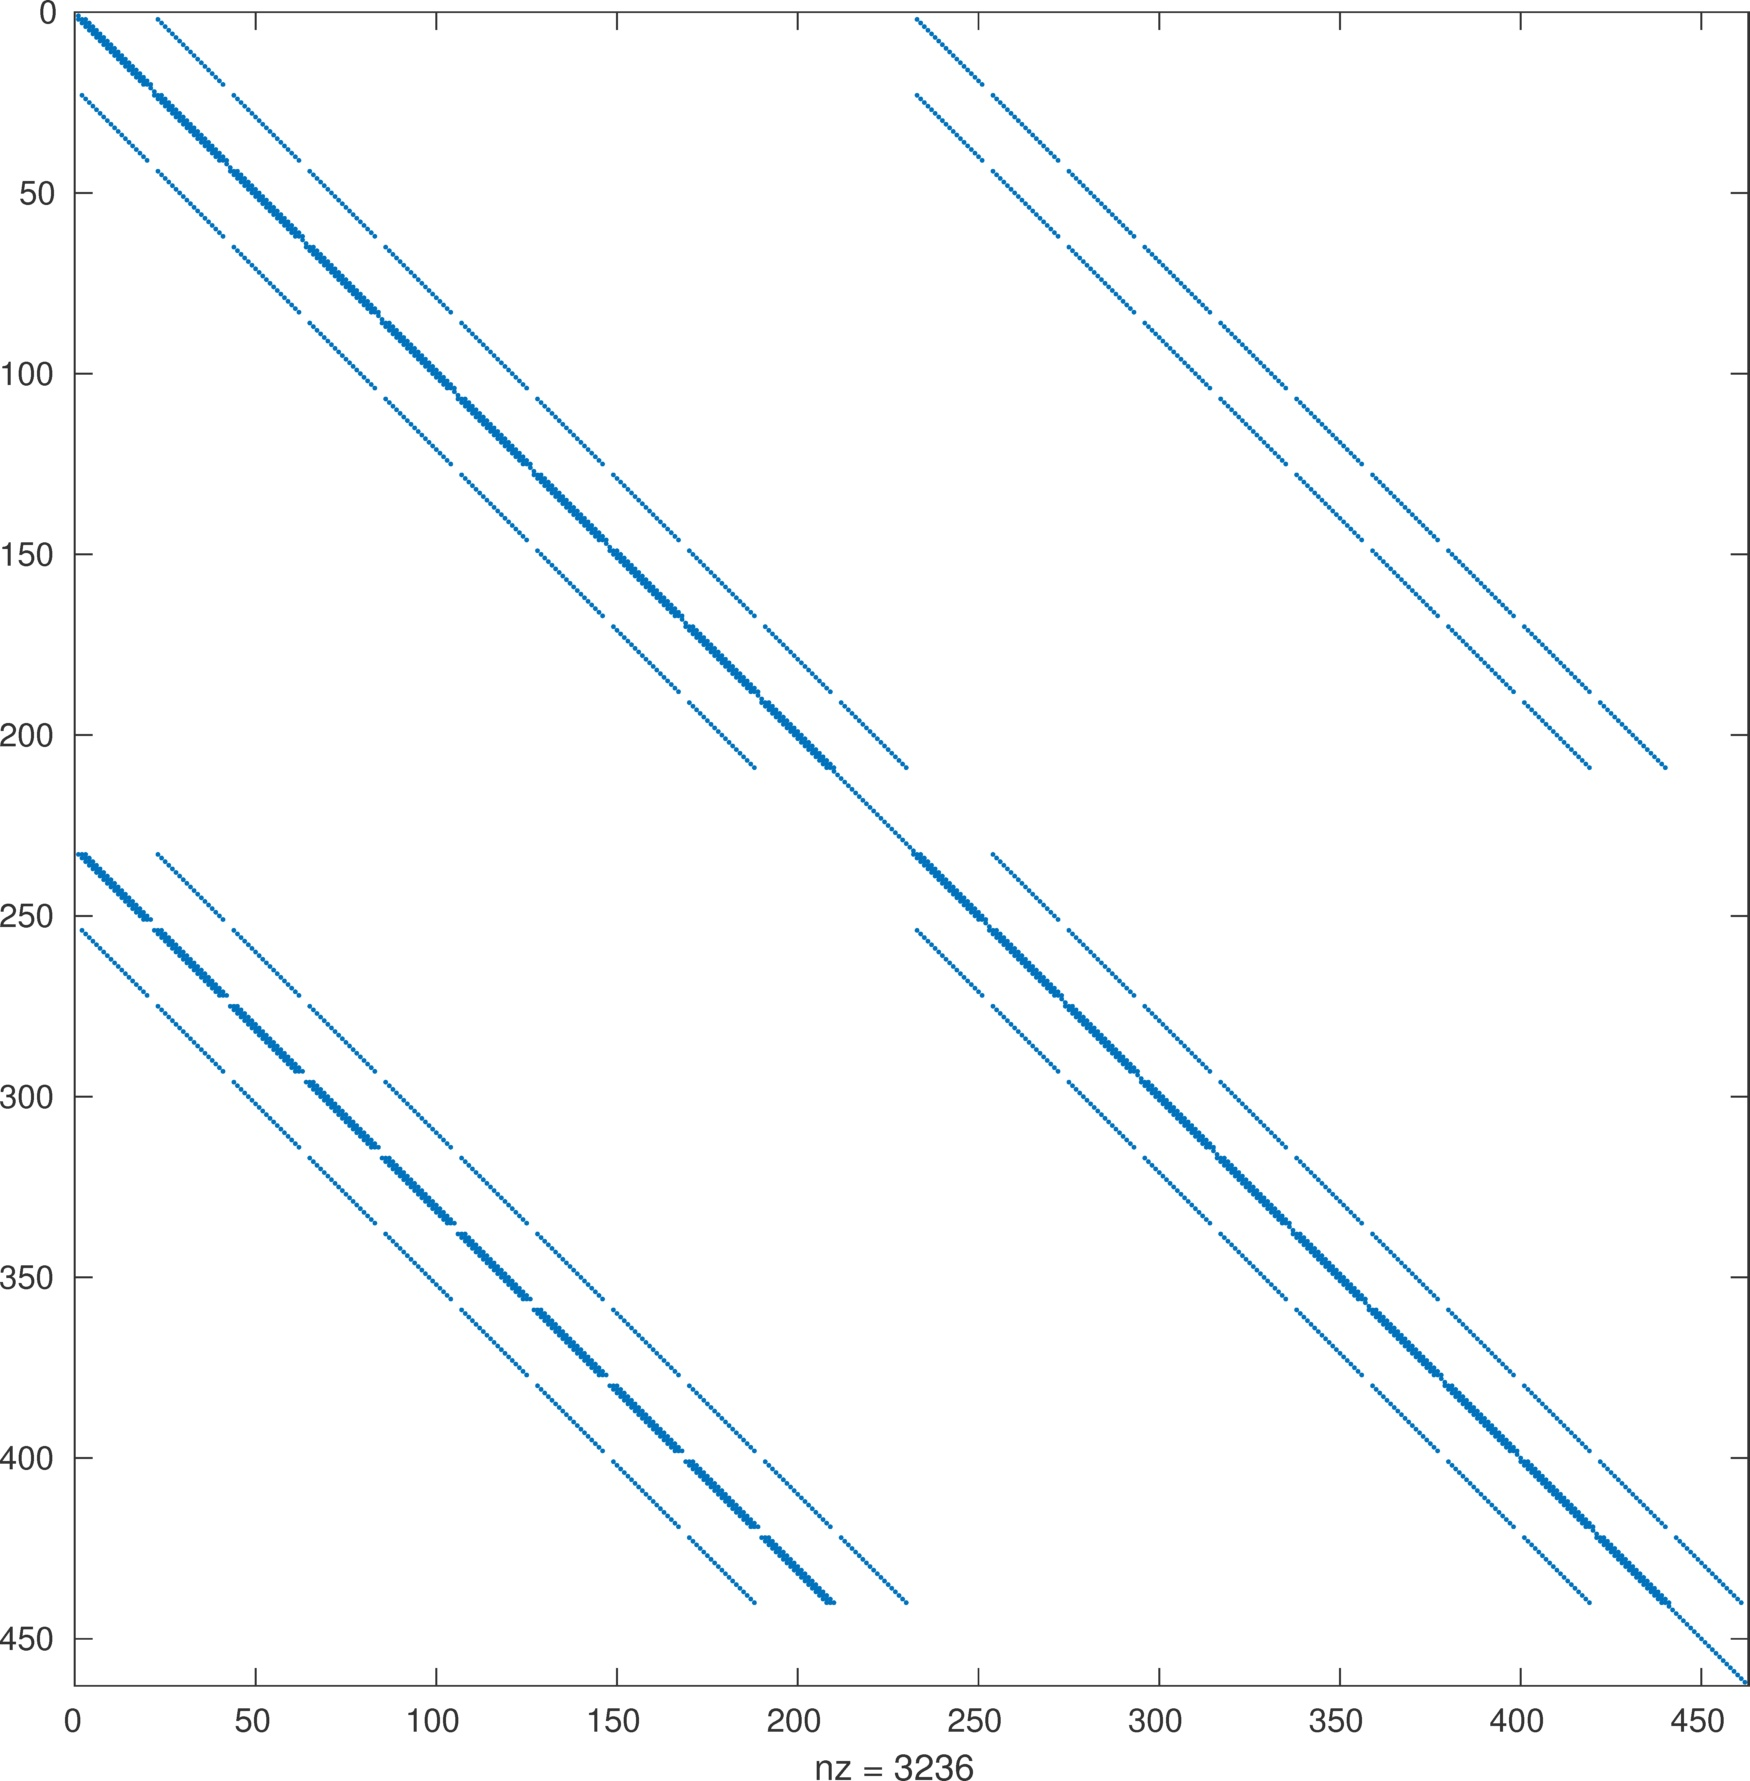
\includegraphics[width=0.6\linewidth]{co2_jac}
\caption{Sparsity pattern of Jacobian matrix~$A$.}%
\label{f:geophysik_J_matrices}
\end{figure}

We solved a system of linear equations with the
coefficient matrix $A$ with the BICGSTAB iterative solver.
We compute the ILU preconditioning on a set of selected elements $S$
instead of the whole Jacobian matrix. 
We compare the convergence histories of the BICGSTAB solver 
on the four different methods of preconditioning:
without preconditioning,
with preconditioning with $S=R_i$,
with preconditioning with $S=R_i + R_a$ in which 
the set $R_a$ is computed based on the greedy coloring,
and with preconditioning with $S=R_i + R_a$ in which 
the set $R_a$ is computed based on the new coloring.

We do this comparison for different block sizes.
The results of the computation of the block size
$10$ and $20$ in
Figure~\ref{f.convergence_greedy_new2} (Top) and
Figure~\ref{f.convergence_greedy_new2} (Bottom), respectively.
In both block $10$ and $20$, the preconditioning computed based
on the new coloring converges in the fewer number of matrix-vector products.
However, it does not mean that the bigger block results always in the 
better convergence.
\begin{figure}
\centering
%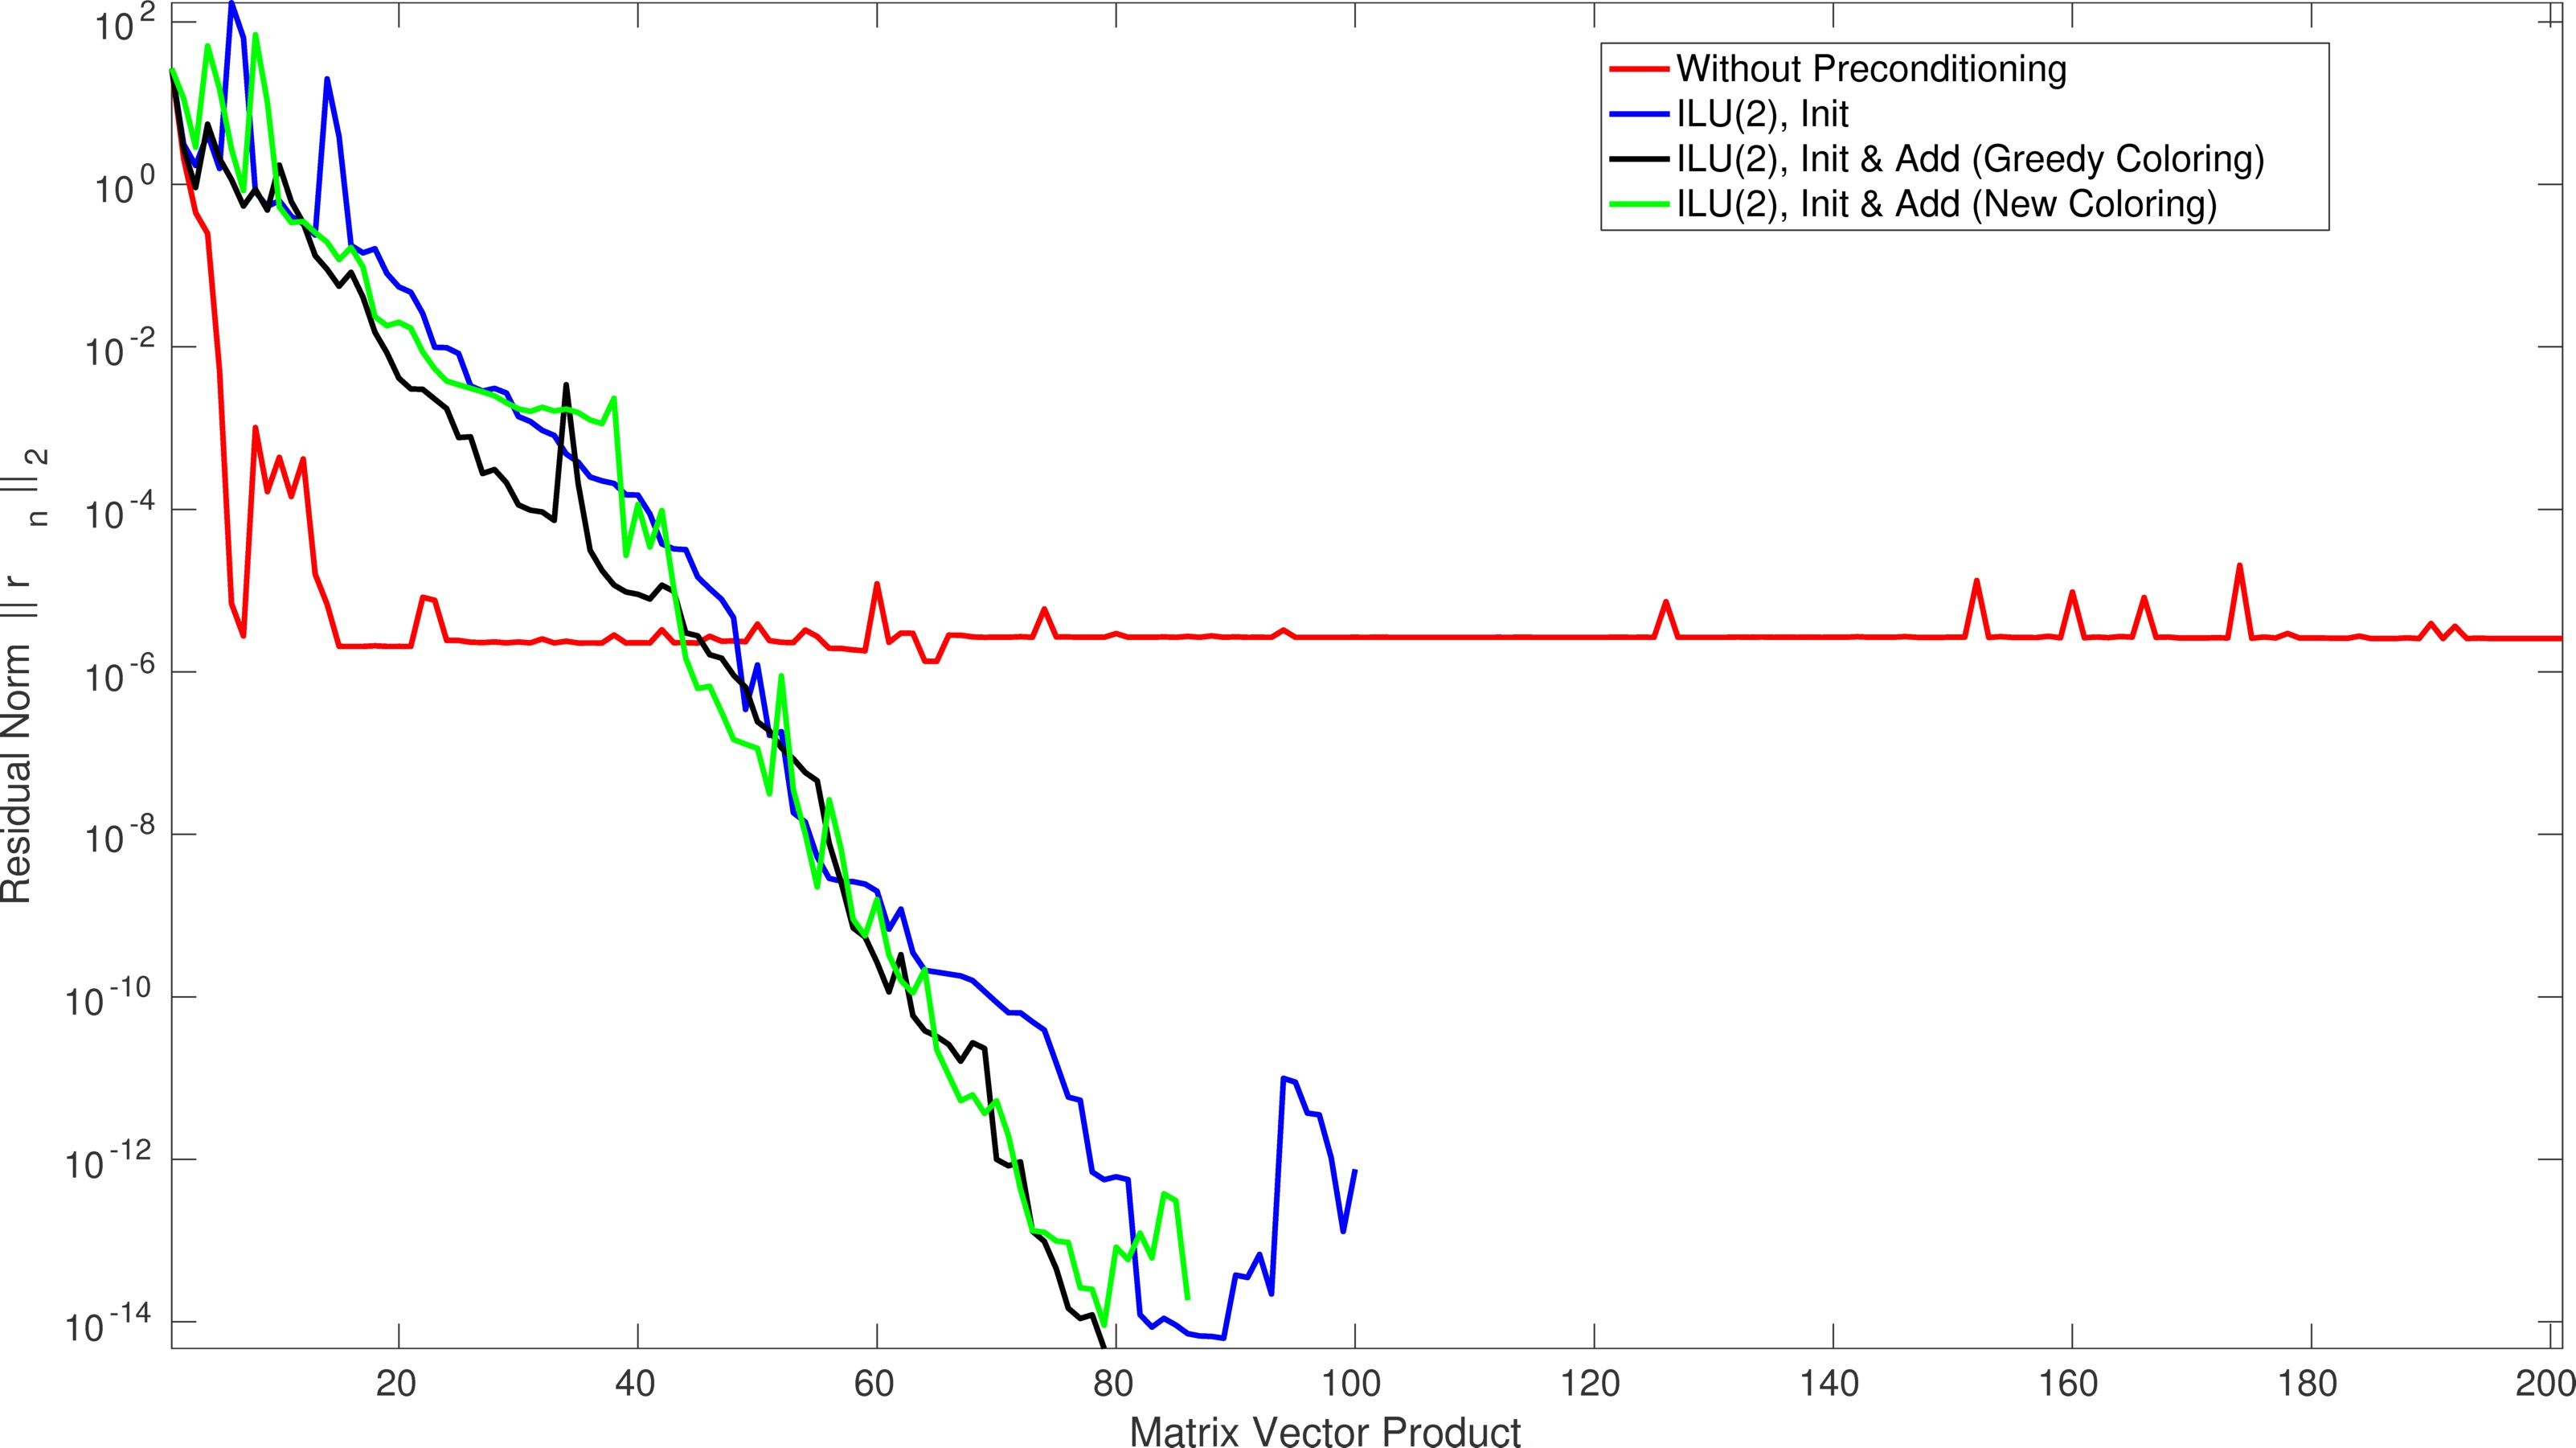
\includegraphics[width=0.8\linewidth]{jac_convergence_greedy_new_bl2.jpg}
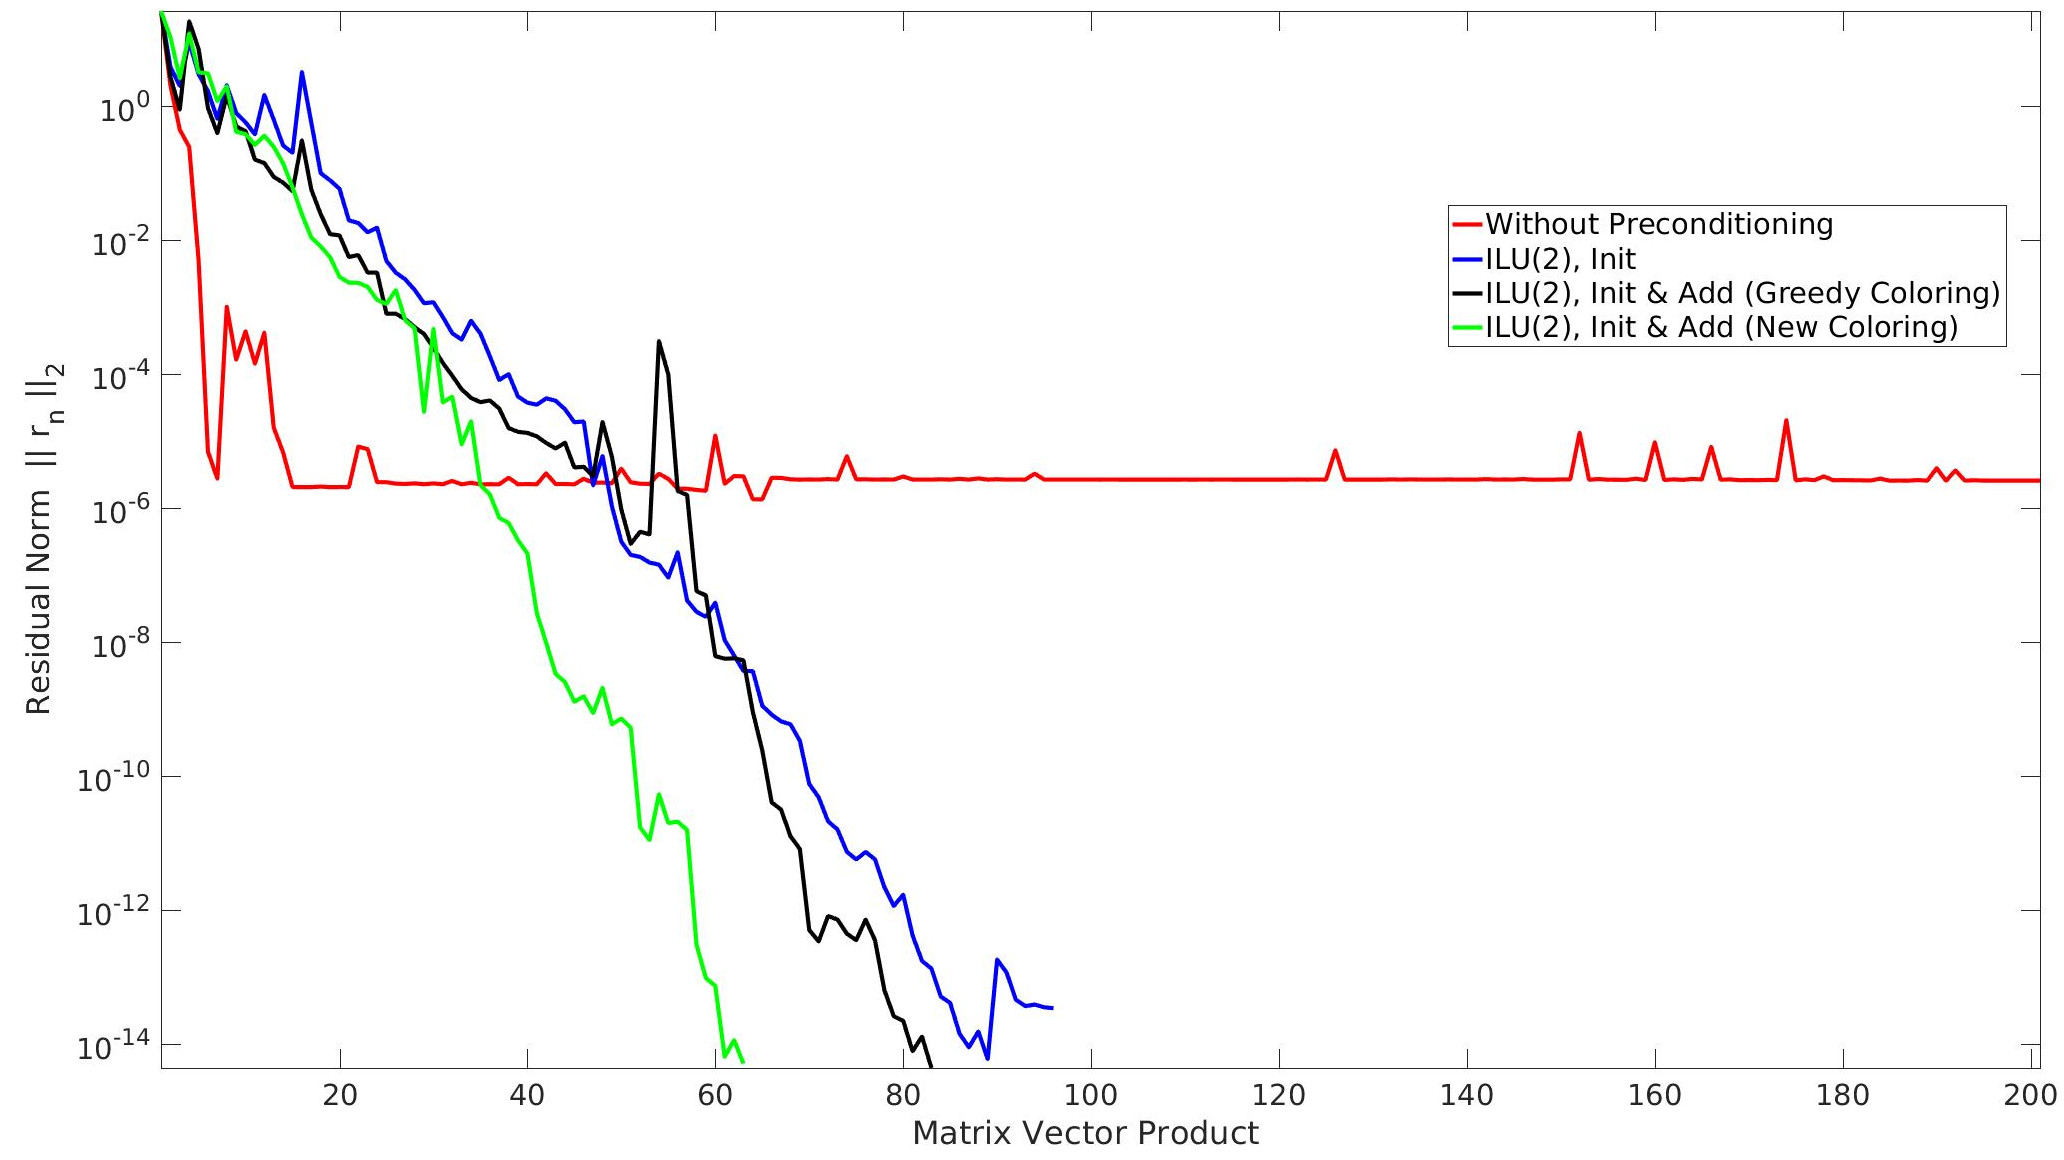
\includegraphics[width=\linewidth]{jac_convergence_greedy_new.jpg}
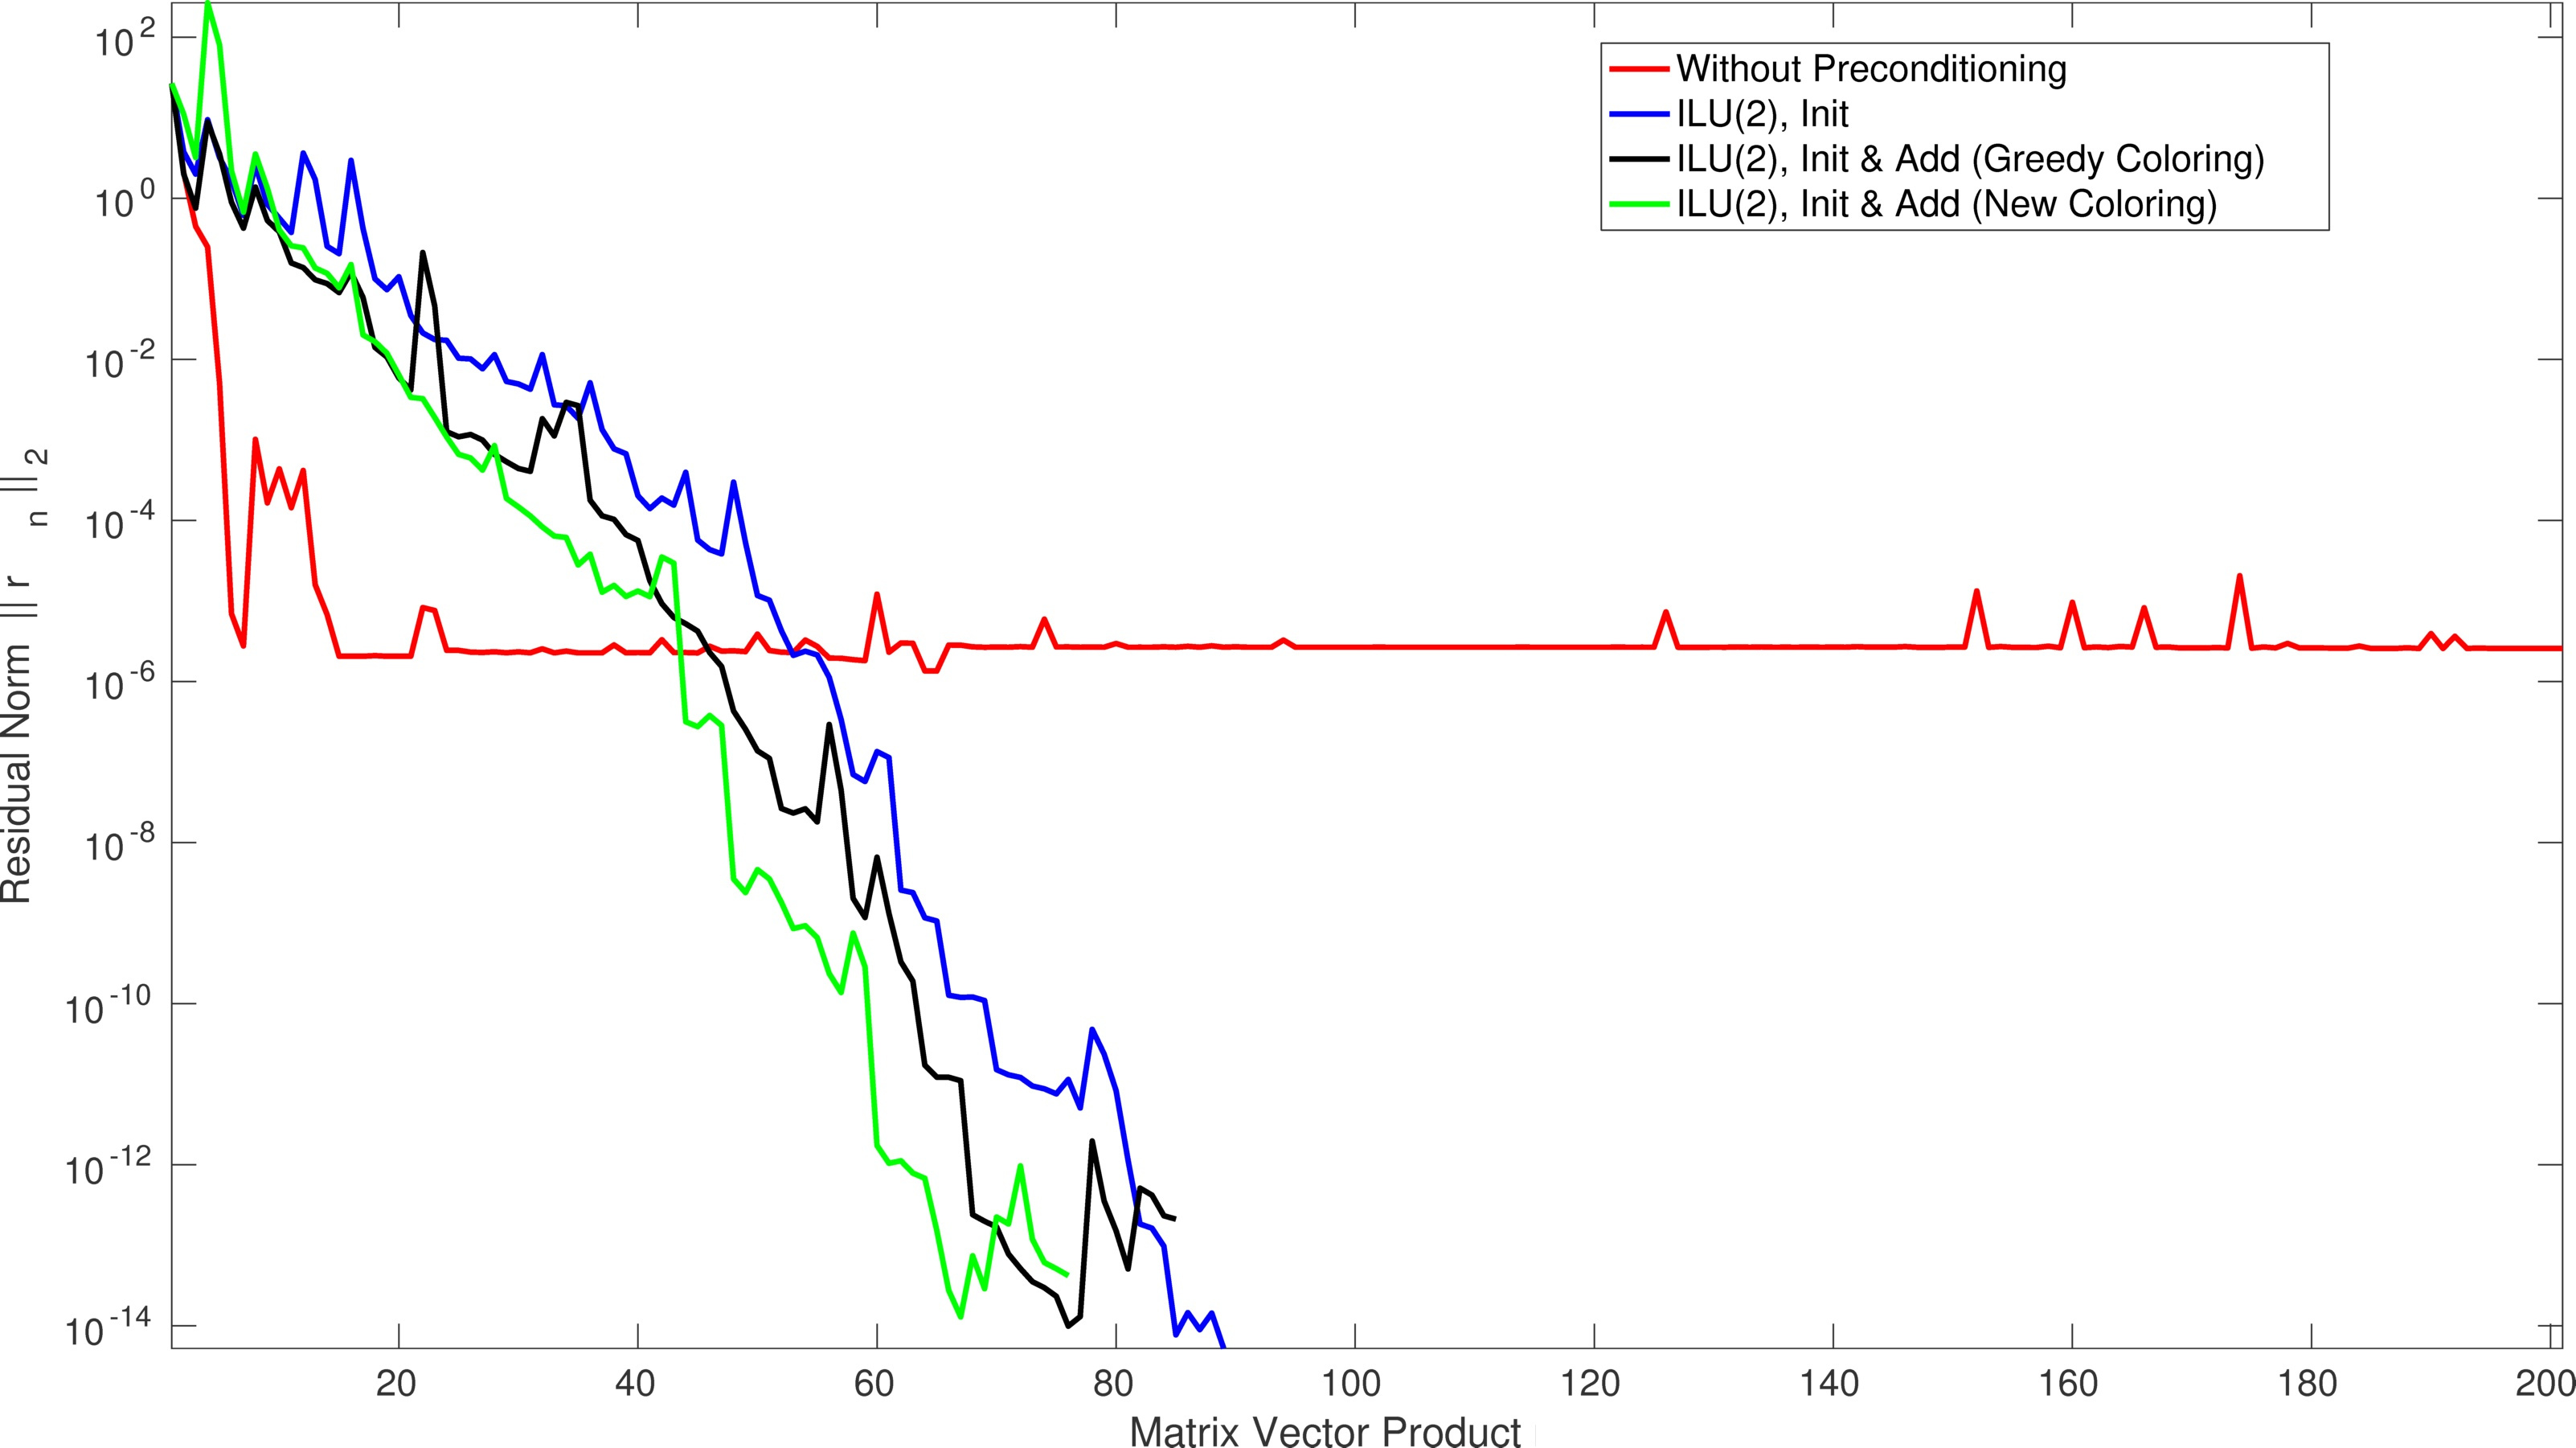
\includegraphics[width=\linewidth]{jac_convergence_greedy_new_bl20.jpg}
\caption{
The history of the residual norms is visualized based on the 
the number of matrix-vector products comparing four different methods:
without preconditioning (red color), 
with preconditioning with $S=R_i$ (blue color),
with preconditioning with $S=R_i + R_a$ in which 
the set $R_a$ is computed based on the greedy coloring (black color),
and with preconditioning with $S=R_i + R_a$ in which 
the set $R_a$ is computed based on the new coloring (green color).
The level parameter of the ILU preconditioning is $2$.
(Top) The block size is $10$. 
(Bottom) The block size is $20$.
}
\label{f.convergence_greedy_new2}
\end{figure}

\clearpage
%%%%%%%%%%%%%%%%%%%%%%%%%%%%%%%%%%%%%%%%%%%%%%%%%%%%%%%%%%%%%%%%%%%%%%%%%%%%%%%%%%%%%%%%%%%%%%
\section{Coloring restricted to diagonal elements}
\label{s.part.color.diag}
%%%%%%%%%%%%%%%%%%%%%%%%%%%%%%%%%%%%%%%%%%%%%%%%%%%%%%%%%%%%%%%%%%%%%%%%%%%%%%%%%%%%%%%%%%%%%%
So far, we consider the partial Jacobian computation with an arbitrary
set of required elements. However, a better heuristics is proposed if the
pattern of the required elements is prior known.
Lülfesmann~\cite{Lulfesmann2012Fap} shows that the minimum number of colors of
the partial star bicoloring restricted to diagonals $\chi_{sb}$ is equal to
the minimal number of colors of the partial distance-$2$ coloring restricted
to diagonals $\chi_{d2}$. It means the bidirectional compression restricting to diagonals is not better than
a distance-$2$ coloring. 
This theorem can be written as two Lemmas,
\begin{itemize}
\item Lemma 1: $\chi_{sb} > \chi_{d2}$
\item Lemma 2: $\chi_{sb} < \chi_{d2}$
\end{itemize}
The proof of Lemma 1 is clear since
a given distance-$2$ coloring with the fewest number of colors is also a star bicoloring.
The proof of Lemma 2 is more tricky. A sketch of the proof comes as follow.
\begin{figure}
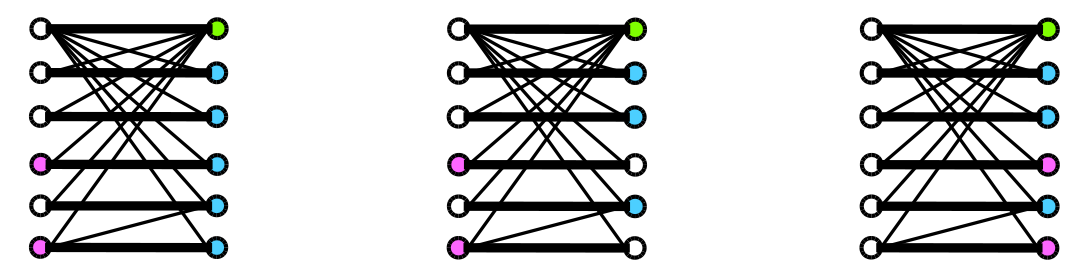
\includegraphics[width=\linewidth]{proof1.png}
\caption{
(Right) An example of a partial star bicoloring restricted to diagonals
transformed to a valid distance-$2$ coloring.}
\label{proof1}
\end{figure}


The idea is to transform a valid star bicoloring with the fewest number of colors $\Phi_{sb}$ to 
a valid distance-$2$ coloring where the number of colors is not larger.
This transformation includes two steps:
\begin{enumerate}
\item The minimal star bicoloring $\Phi_{sb}$ is transformed 
to the valid star bicoloring $\Phi_{sb}^{*}$ 
where exactly one of both incident vertices of each required edge is colored nonzero.
\item The valid coloring $\Phi_{sb}^{*}$ is transformed 
to the valid star bicoloring $\Phi_{sb}^{'}$ where all row vertices are colored by zero.
This star bicoloring is also a distance-$2$ coloring.
\end{enumerate}
An example of this transformation can be seen in \figref{proof1}. 

Looking at the proof, this theorem can be generalized by considering any
coloring instead of the optimal coloring.
On the other hand, the set of diagonal elements in the theorem
can be replaced by any set of required elements
in which each column and row contain only one required nonzero elements.
This property is nothing than a matching~\cite{bondy2008graph} in a graph language.
Given a graph and the vertex and edge set $G=(V,E)$, a matching $M\subset E$ contains
a list of edges which do not have any vertex in common.
A maximum matching is a matching with a maximum possible number of edges.
Then, a diagonal for example in our bipartite graph is a maximum matching.

Now, we can formulate a new theorem on the comparison of one directional and
bidirectional coloring as follows,
\begin{theorem}
\label{t.matching}
Given the bipartite graph $G=(V_r\cup V_c,E)$ and a matching $M\subset E$ representing
the required elements, any valid partial star bicoloring $Q_{sp}$ restricted to $M$
with the number of colors $\chi_{sp}$
can be transformed to a valid distance-$2$ coloring restricted to $M$
with the number of colors $\chi_{d2}$ such that $\chi_{sp} \leq \chi_{d2}$.
These numbers of colors can be different than the minimal number of colors.
\end{theorem}
This theorem is a generalization of Theorem 3.7 of \cite{Lulfesmann2012Fap}.
Theorem 3.7 of \cite{Lulfesmann2012Fap} discusses only the mapping with minimal coloring
and the coloring restricted to diagonal elements. We consider any coloring
and the coloring restricted to a matching. This generalization gives us an idea
to find new heuristics for coloring. The proof of Theorem~\ref{t.matching}
is resulted from the proof from \cite{Lulfesmann2012Fap} considering two following points,
\begin{itemize}
\item The minimality of mappings are only used to show the equality in the number of colors which is not
the case in our theorem.
\item The property of being diagonal elements are used in the proof from \cite{Lulfesmann2012Fap} only to
make the required edges disjoint from each other which is the definition of a matching in graphs.
\end{itemize}

Based on the column-intersection graph model presented in \cite{cscpaper},
it is easy to see
that the coloring restricted to diagonal is still an NP-complete problem.
In this paper, a classical graph coloring problem on an undirected graph
is formulated from the partial Jacobian computation.
We know that a graph coloring is an NP-complete problem
(see \cite{np-complet-graph-coloring})).
So the coloring restricted to the diagonal elements should be NP-complete too.

Therefore, we should still use some heuristics to compute these colorings.
The examples in Table~\ref{table.starbic.d2.diag} from Florida sparse collection shows that the
inequality in Theorem~\ref{t.matching} can happen. The second column of this table
shows the number of colors computed by the heuristic for star bicoloring.
The third column shows the number of colors computed by the greedy distance-$2$ coloring
in which the minimum number of colors between the row and column version is selected.
It can be seen that even for a small matrix as the matrix \textit{cage3} which has only
$5$ rows and columns, the star bicoloring can produce a better result.
However, the difference between the number of colors is not so high for these examples.
So, it is not maybe efficient to run the star bicoloring to get a better coloring for
the one-sided coloring. Hence, a new heuristic is proposed with a lower complexity
to compute the same coloring.
\begin{table}
\centering
\begin{tabular}{|c|c|c|}
\hline
Matrix & $\Phi_{sb}$ & min($\Phi_r$,$\Phi_c$)\\\hline
\textit{cage3} & $3$ & $4$\\\hline
\textit{cage4} & $3$ & $4$ \\\hline
\textit{cage5} & $5$ & $7$\\\hline
\textit{cage7} & $7$  & $8$\\\hline
\textit{cage8} & $8$  & $10$\\\hline
\textit{cage9} & $9$  & $11$\\\hline
\textit{cage10} & $10$ & $11$\\\hline
\textit{cage12} & $13$ &  $14$\\\hline
\end{tabular}
\hfill
\begin{tabular}{|c|c|c|}
\hline
Matrix & $\Phi_{sb}$ & min($\Phi_r$,$\Phi_c$)\\\hline
\textit{ex7} & $18$ & $22$ \\\hline
\textit{nos3} & $10$ & $10$ \\\hline
\textit{steam1} & $6$ & $6$ \\\hline
\textit{steam2} & $8$ & $8$ \\\hline
\textit{rajat01} & $8$ & $8$ \\\hline
\textit{gyro\_m} & $15$ & $15$\\\hline
\textit{ex33} & $12$ & $11$\\\hline
\textit{cavity16} & $20$ & $18$ \\\hline
\end{tabular}

\caption{The comparison of number of colors in star bicoloring and in
distance-$2$ coloring restricted to diagonals.
The ordering is the natural ordering of the matrix for the both colorings.
%the value of $\alpha$ is equal $1.0$
}
\label{table.starbic.d2.diag}
\end{table}

We have developed some ideas based on Theorem~\ref{t.matching}
for a better heuristic. The idea is that a heuristic for star bicoloring maybe
find a better coloring because of the inequality in the theorem.
As theorem proposes, every required nonzero element
is determined by either a column or a row and not both. Hence, a heuristic
can iterate on the required element and selects between the row and column of
the nonzero in favor of minimal coloring.
Thus, the star bicoloring heuristic can be rewritten for a better computational complexity.
Regarding these ideas, the star bicoloring is rewritten as in \coderef{star.diagonal}.
\begin{figure}
\begin{lstlisting}[
caption=An improved star bicoloring restricted to diagonal elements.
As the theorem says this coloring generates an equivalent distance-$2$ coloring.,
label=star.diagonal,mathescape]
function star_diag($G=(V_r\cup V_c)$, $E_R$)
  for $v\in V_c$
    $\Phi(v)=-1$
    $forbiddenColors1[v] = 0$
    $forbiddenColors2[v] = 0$

  for $e=(v,u)\in E_R$
    $forbiddenColors1[0] = v$
    $forbiddenColors2[0] = u$

    for $n\in N2(G,v)$
      if $\Phi(n) > 0$
        $forbiddenColors1[\Phi(n)] = v$

    forbiddenColors[0] = u;
    for $n\in N2(G,u)$
      if $\Phi(n) > 0$
        $forbiddenColors2[\Phi(n)] = u$

    $c_1 = min(\{j>0: forbiddenColors1[j] \neq v\})$
    $c_2 = min(\{j>0: forbiddenColors2[j] \neq u\})$

    if $c_1 < c_2$
      $\Phi(v) = c_1$
    else
      $\Phi(u) = c_2$

    for $v\in V_c$ with $\Phi(v)>0$
      $\Phi(v) = \Phi(v) + max(\{ \Phi(u):u\in V_r \})$

    for $v\in V_r\cup V_c$ with $\Phi(v) = -1$
      $\Phi(v) = 0$
\end{lstlisting}
\end{figure}

%%%%%%%%%%%%%%%%%%%%%%%%%%%%%%%%%%%%%%%%%%%%%%%%%%%%%%%%%%%%%%%%%%%%%%%%%%%%%
\section{A new heuristic based on exact coloring of small subgraphs}
\label{s.exact}
%%%%%%%%%%%%%%%%%%%%%%%%%%%%%%%%%%%%%%%%%%%%%%%%%%%%%%%%%%%%%%%%%%%%%%%%%%%%%
As discussed in \cite{Fomin2013}, a prominent approach used by various graph coloring
algorithms is based on finding independent sets. A subset of the vertices $S\subset V$ is
called an independent set if there is no edge between any of these vertices, i.e.,
$$
\forall u,v\in S: (u,v)\notin E.
$$

An exhaustive search iterating over all possibilities to color the $n$ vertices using $k$
colors has the computational complexity $k^n$. However, the dynamic programming approach
can improve this computational complexity. The fastest exact algorithm of graph coloring is proposed by
Bj{\"o}rklund, Husfeldt, and Koivisto~\cite{bjorklund2009} and has the complexity
$O(2.2416^n)$. The idea behind this novel algorithm is based on the principle of
inclusion and exclusion, which leads to the following definition.

Let $A$ and~$B$ denote two sets whose elements are also sets. Their product, $A\times B$,
is then defined as
$$
A\times B := \bigcup_{a\in A, b\in B}{a \cup b}.
$$
For example, if $A=\bigl\{ \{1\}, \{3,4\} \bigr\}$ and $B=\bigl\{ \{2\}, \{3,5\} \bigr\}$, then
their product is given by
\begin{equation}
\label{eq:axb}
A \times B=\bigl\{ \{1,2\}, \{1,3,5\}, \{2,3,4\}, \{3,4,5\} \bigr\} .
\end{equation}

The graph coloring algorithm proposed in \cite{bjorklund2009} consists of computing $k$
products of a set $I$, i.e.,
$$
I^k := I \times I  \times \cdots \times I .
$$
Here, $I$ is the set of all independent sets of the graph~$G$. Then, the chromatic number
of $G$ is shown to be the smallest~$k$ such that $V\in I^k$.

In general, larger powers of $I$ are necessary for the solution of graph coloring
problems. We stress that these powers may be difficult to compute. An elegant way
introduced in~\cite{bjorklund2009} is to compute these powers via zeta transforms. The
underlying idea is based on first transforming a set $A$ into its zeta transform defined
by
$$
Z(A) := \cup_{a \subset A} a.
$$
The product $A \times B$ is then computed by first transforming $A$ and $B$ into $Z(A)$
and $Z(B)$ and then using the identity
$$
A\times B = Z^{-1} \bigl( Z(A) \cup Z(B) \bigr)
$$
where the inverse of the zeta transform can be defined similarly. This way, the product
of sets is transformed into a union of sets in the zeta space. Finally, there is a way to
compute a zeta transform and its inverse efficiently by means of a so-called fast zeta
transform \cite{Knuth:1997:ACP:270146}.

Here, we introduce a new heuristic based on this exact coloring.
The idea is to divide a large graph to small subgraphs and apply an exact coloring
on these small subgraphs. Then, integrate the remaining parts into these colored
subgraphs.
More clearly, these are the steps which we follow,
\begin{itemize}
\item find a vertex separator for example by the nested dissection algorithm
\item remove the vertex separator
\item find the exact coloring of the remaining components separately
\item color the subgraph of vertex separator in the original graph considering
the computed exact coloring in the remaining components 
\end{itemize}

A question is if it gives a better coloring at all since the coloring of vertex separator
can lead us to a worse coloring.
We build an example in which we found a better coloring by the second strategy.
We first build a graph and its heuristic coloring which generates a worse coloring
than an exact coloring as shown in~\figref{f.coloring.graph} (Left). If we follow
the numbering of the vertices as the ordering for a greedy coloring, we need
at least $4$ colors while the exact coloring needs only $3$ colors.
Now, we make a copy of this graph and add an extra vertex $15$ as in
~\figref{f.coloring.graph} (Right). The vertex $15$ is the only element of
a vertex separator for the new graph. We added the incident edges of $15$ such that
the resulting graph becomes a worst case for the greedy coloring here.
In this new graph, the greedy coloring needs at least $5$ colors
as in~\figref{f.coloring.compared} (Left).

Suppose we color first the components after removing the vertex $15$ separately with
an exact coloring which needs only $3$ colors. Now, even a bad implementation of the
new idea would need $4$ colors, i.e., one colors fewer than the greedy algorithm.
A good implementation color the graph only with $3$ colors.
The construction of given example can go further by creating several copies of 
this graph, make the separator part a complete graph, and connect the separator vertices
with same fashion to each copy.
\begin{figure}
\centering
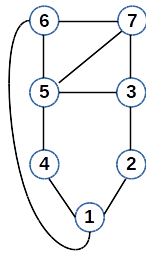
\includegraphics[width=0.18\linewidth]{coloring0}
\hfill
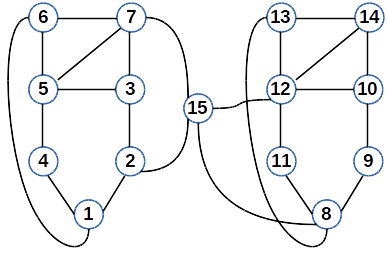
\includegraphics[width=0.48\linewidth]{coloring1}
\caption{
An example of a graph in which the division into two parts can be seen directly.
The numbering of the graph vertices are the ordering that the greedy coloring follows.
}
\label{f.coloring.graph}
\end{figure}

\begin{figure}
\centering
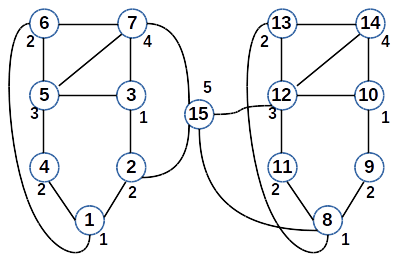
\includegraphics[width=0.48\linewidth]{coloring2}
\hfill
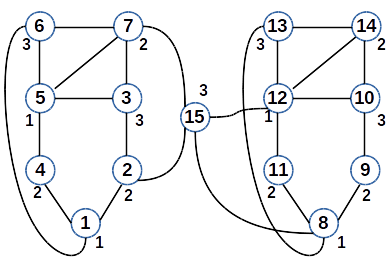
\includegraphics[width=0.48\linewidth]{coloring3}
\caption{Comparison of colorings by a greedy coloring and
by the new suggested coloring.}
\label{f.coloring.compared}
\end{figure}

We saw that large powers of $I$ are computed during the algorithm.
The storage size increases dramatically when the number of vertices
in the graph increases. To solve the storage size, we consider each 
subset as a binary number as follows. A binary number in which
the number of bits is the number of vertices, represents a subset.
It means if the $i$th bit is $1$ then the $i$th element is in that subset.
We used the class \text{bitset} from C++ to decrease the memory usage as much
as possible.

For a further evaluation of this algorithm, we use the toolbox \textit{MESHND}
of MATLAB to generate a set of matrices and their equivalent nested dissection ordering.
The command \textit{meshnd($m$,$n$,$k$)} constructs an $m$-by-$n$-by-$k$ 3D mesh $M$
and computes the nested dissection ordering of the corresponding sparse matrix.
To get the corresponding sparse matrix, we need to call the command 
\textit{meshsparse($M$,$S$)} in which the variable $S$ specifies the size
of the stencil.
Table~\ref{table.exact.greedy} compares the number of colors in our new 
heuristics considering the exact coloring on subgraphs $\chi_{x}$ and 
the number of colors in the greedy coloring.
\begin{table}
\centering
\begin{tabular}{|c|c|c|c|c|c|}
\hline
Matrix & Size & Nonzeros & Stencil & Greedy Coloring & $\chi_{x}$ \\\hline
\textit{meshnd(10,10,4)} & $400$ & $1740$ & $7$ & $14$ & $12$\\\hline
\textit{meshnd(10,10,5)} & $500$ & $3100$ & $7$ & $15$ & $12$\\\hline
\textit{meshnd(5,10,10)} & $500$ & $3100$ & $7$ & $15$ & $12$\\\hline
\textit{meshnd(10,10,10)} & $1000$ & $6400$ & $7$ & $16$ & $13$\\\hline
\textit{meshnd(20,20,20)} & $8000$ & $53600$ & $7$ & $15$ & $13$\\\hline
\textit{meshnd(20,30,40)} & $24000$ & $162800$ & $7$ & $17$ & $13$\\\hline
\textit{meshnd(20,20,20)} & $8000$ & $67280$ & $9$ & $16$ & $10$\\\hline
\textit{meshnd(20,30,40)} & $24000$ & $204160$ & $9$ & $17$ & $10$\\\hline
\end{tabular}
\caption{The number of colors in the new heuristics considering the exact coloring on subgraphs
compared with the number of colors in the greedy coloring.}
\label{table.exact.greedy}
\end{table}

%Although this algorithm seems convincing, the computation of nested dissection is still
%a tricky part.


%%%%%%%%%%%%%%%%%%%%%%%%%%%%%%%%%%%%%%%%%%%%%%%%%%%%%%%%%%%%%%%%%%%%%%%%%%%%%
\section{The computational package: PreCol 1.0}
\label{s.extend}
%%%%%%%%%%%%%%%%%%%%%%%%%%%%%%%%%%%%%%%%%%%%%%%%%%%%%%%%%%%%%%%%%%%%%%%%%%%%%
We develop a piece of software to implement our proposed heuristics.
Specially, the software is designed employing concepts from the object-oriented programming
such that it can be extended later with any new coloring heuristic as well as any preconditioning algorithm.
The developers can implement new extensions without going into details of core implementation.
Two main ingredients coloring and orderings can be implemented now only by deriving an interface.
For example, a new coloring and ordering can be added as easy as the following code.
\begin{lstlisting}
class New_Ordering : public Ordering {
  bool order(const Graph &G, vector<unsigned int> &ord, bool restricted) {...}
};

class New_Coloring : public ColAlg {
  int color() {...}
};
\end{lstlisting}

The developer needs to implement this new class in an only-header fashion~\cite{headeronly},
since the goal is to write an extension with a few code. So, the developer should
move the new header file to the corresponding directory which is the ordering directory
for this new ordering and \textit{algs} directory for coloring algorithms.
Now, building the software would bring this new ordering into the software execution.

The input matrix is in the format of the matrix market~\cite{matrix-market}. 
After reading this matrix, we convert it to the different graph models 
like a column-intersection graph or a bipartite graph. 
Any result matrix like the sparsified matrix also will be saved in this file format.

\textit{PreCol} is developed in \textit{C++} using STL (the standard library) and
the boost library\cite{boost}.
Using new concepts of functional programming
in new C++ release~\cite{Sutherland2015}, we provide different functions which can be used
by developer to work on graphs. For example, the iteration of vertices
or edges can be easy as follows,
\begin{lstlisting}
for_each_v(G, f);
for_each_v(G, [&](Ver v) {...});
for_each_e(G, f);
for_each_e(G, [&](Edge e) {...});
\end{lstlisting}
, in which the variable $f$ is a function which gets an input parameter
of a vertex or an edge, respectively.
Also, the other syntax is the lambda function
from the new C++ functional programming to implement a function in place.

Following a unique solution, we implement all the possible part of algorithms
with the use of standard library of C++ which also improves the readability.
This strategy reduces the amount of the code dramatically and
make the code more readable.
Also, the standard algorithms would be automatically parallel in the next
release of C++ (C++17) next year~\cite{parallelcpp}.

As it is presented in \figref{f.structure}, both computations of coloring and ILU preconditioning
are in one package available in C++. we also introduced
two interfaces in MATLAB and JAVA languages which we will explain in
Section~\ref{s.interfaces}.
%-----------------------------------------------------------------------------------------------
\begin{figure}
\centering
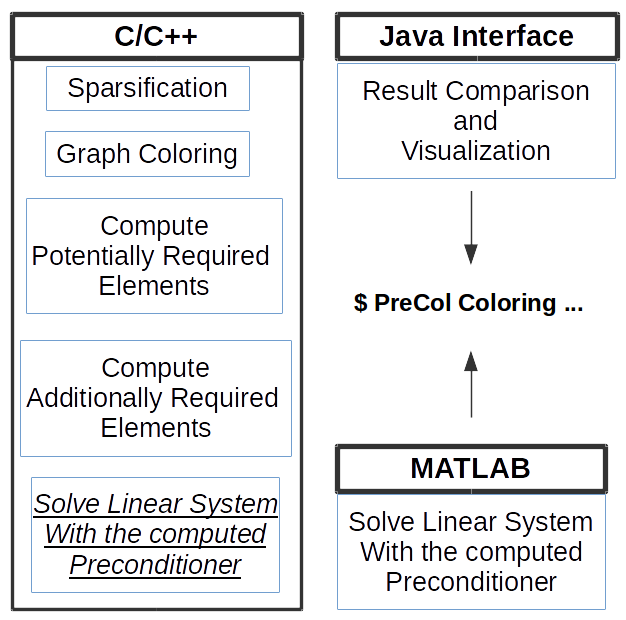
\includegraphics[width=0.52\textwidth]{new_struct}
\caption{
The software PreCol and its two interfaces written in MATLAB and Java are visualized.}
\label{f.structure}
\end{figure}
%-----------------------------------------------------------------------------------------------

To use the software, the user can use a command-line command in addition to
the interfaces in JAVA and MATLAB. So, the user needs to specify different
options for coloring algorithms, orderings, the block size, and so.
These options can be entered directly in the terminal together with command.
An example is as follows,
\begin{lstlisting}
precol PartialD2RestrictedColumns LFO_Nat BlockDiagonal 30 2 ex33.mtx
\end{lstlisting}
in which the \textit{PartialD2RestrictedColumns} is the coloring algorithm,
two strings of \textit{LFO} and \textit{Nat} are for the coloring and ILU ordering.
The next parameter \textit{BlockDiagonal} specifies the sparsification method
which is followed by the size of the block $30$. The next number $2$ specifies
the level parameter of ILU and finally comes the matrix name.

We also generated a new documentation as a website which is available
under the website: http://csc.c3e.de/precol/html.
This website is generated automatically by Doxygen~\cite{Lischner2013}.
We implemented some new HTML/CSS template for doxygen to include extra
texts and documentation in the website.

%\todo{zero or one}
%mohem ... discussion about the sparsification in MATLAB and C/C++
%staring from zero or one ???

\subsection{User interfaces}
\label{s.interfaces}
We extend our JAVA software GraphTea~
\cite{2014:07,2014:15,2014:16,2015:05,2015:06,2015:07,2015:08} to have a
set of reports for graph coloring and preconditioning. It has two different modes
to compute independently or to call the software \textit{PreCol}.
%Chemical Graph theory\cite{2015:05,2015:06,2015:07,2015:08}
GraphTea is a graph editing framework designed specifically to compute and visualize
different parameters of graphs interactively.
Figure~\ref{f.graphtea} shows a snapshot of the
graph window together with two additional windows that give more details on the solution
of different graph problems. These separate windows providing additional information are
called ``reports.''

A report can be computed in GraphTea in two different ways:
a single report or an incremental report.
A single report means to compute some parameters on graph and look at the results
in a textual way. However, an incremental report happens when we have at least
two parameters for computation. So, we change one of the parameters in
some range and would generate a table.

The primary goal of developing GraphTea is to support the researcher through their research.
The following abilities of GraphTea could help the research in different dimensions:
\begin{itemize}
\item Generate different class of graphs and compute the parameters on them.
\item Get reports on the graph beside the parameter and find the connections.
\item Compute the operations on graphs and influence of these operations on parameters
of the graph.
\end{itemize}

If we divide the researcher's works follows,
\begin{enumerate}
\item Guess a hypothesis like a bound for coloring number
\item Evaluate this bound on different graphs
\item Prove the hypothesis
\end{enumerate}
The second step, i.e., evaluation, is always an important step since many first errors and
improvements could be found.
However, the researcher can only do this evaluation for small examples if they do not
use computer tools.
Different aspects of GraphTea can be used to overcome this evaluation.
The researchers can generate any graph up to any computationally-reasonable size
and compute the parameter.
This process of so-called conjecture checking on different graphs could often lead to a better guess.
%-----------------------------------------------------------------------------------------------
\begin{figure}
\centering
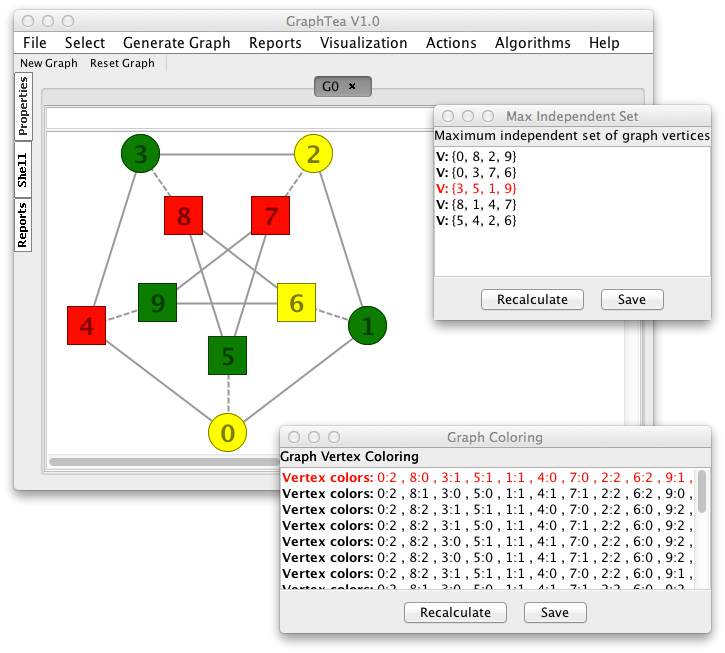
\includegraphics[width=0.7\textwidth]{graphtea}
\caption{An overview of GraphTea: A graph drawing window and
two floating dialogs with reports on a given graph.}
\label{f.graphtea}
\end{figure}
%-----------------------------------------------------------------------------------------------

Beside the automatic generation of graphs up to any size, we added the ability of loading
different sparse matrix as graphs to GraphTea.
A new data structure for the sparse matrix, called \textit{SpMat}, is designed
to handle the large sparse matrices. This data structure is an array.
The size of this array is the number of rows. Each cell of this array points to
an array which is the corresponding columns of nonzeros in this row.

The MATLAB interface is just a wrapper function which calls \textit{precol} with
the same number of parameter as follows,
\begin{lstlisting}
function [req,pot,add,F,num_col] = precol(coloring,
	coloring_order,ilu_order,block_size,ILU_level_parameter,MatrixName,alpha)
...
end
\end{lstlisting}
%%%%%%%%%%%%%%%%%%%%%%%%%%%%%%%%%%%%%%%%%%%%%%%%%%%%%%%%%%%%%%%%%%%%%%%%%%%%%%%%%%%%%
\chapter{Interactive educational modules}
\label{explain}
%%%%%%%%%%%%%%%%%%%%%%%%%%%%%%%%%%%%%%%%%%%%%%%%%%%%%%%%%%%%%%%%%%%%%%%%%%%%%%%%%%%%%
We develop an extensible collection of educational modules (\mbox{EXPLAIN})
to teach combinatorial scientific computing in classroom.
There is an increasing need for such educational tools since the connection
between the problems from scientific computing and the corresponding combinatorial
problem is tricky for the students. This chapter summerizes our previous publications
\cite{2013:05,2014:01,2014:02,2014:09,2015:3} and also provides some new features.

Since graphs are ubiquitous in computer science, mathematics, and a variety of other scientific
disciplines there are plenty of software tools for teaching graph-theoretical topics and graph
algorithms. However, to the best of the authors' knowledge, there is no other software than EXPLAIN
that provides the simultaneous visualization of a graph and a matrix next to each other. This
overall layout of EXPLAIN is crucial to better understand the relationship between the graph
problem and the corresponding matrix problem. These two different views of the same problem are
critical for establishing an understanding of the problem at hand.

Though there is no previous work directly related to that area, we shortly mention the Gato/CATBox
\cite{gato2002} software whose focus is on animation of graph algorithms. Similarly, the
CABRI-Graph \cite{CABRI96} software is mainly used for algorithm visualization. There are also many
software tools in the area of information visualization like
Tulip~\cite{auber:tulip3,tulippython2012} that visualize and analyze graphs. However, all these
graph software tools do not involve any aspects of scientific computing. On the other hand,
existing tools with a focus on scientific computing do not involve any aspects from graph theory.
Examples include the interactive Java applets devoted to the textbook by Heath~\cite{MH96SCAIS} and
the NCM software to be used in conjunction with the textbook by Moler~\cite{mol:num}.

During this chapter, we first look at the concept and design of the software in
\secref{s.concept}. Then, we apply the gamification ideas on the software in
\secref{s.game} to involve the students more into the usage of \mbox{EXPLAIN}.
After looking at the available modules in \secref{s.av.modules}, we look at
implementation details in \secref{s.impl.explain}.
\mbox{EXPLAIN} has two releases 1.0 and 2.0 which we will explain in more
detail in \secref{s.impl.explain}. Some of the modules
are only available in the new release. Both releases
are available now since they were developed on different technologies and have
pros and cons. However, the release 2.0 is an improved version and is developed
regularly.
%%%%%%%%%%%%%%%%%%%%%%%%%%%%%%%%%%%%%%%%%%%%%%%%%%%%%%%%%%%%%%%%%%%%%%%%%%%%%%%%%%%%%
\section{Concept and design}
\label{s.concept}
%%%%%%%%%%%%%%%%%%%%%%%%%%%%%%%%%%%%%%%%%%%%%%%%%%%%%%%%%%%%%%%%%%%%%%%%%%%%%%%%%%%%%
Throughout the design stage of \mbox{EXPLAIN}, our focus is on the following goals.
\mbox{EXPLAIN} is not a self-study tool.
Rather, the connection between the scientific computing
and combinatorial problems is explained by a teacher in classroom.
The students can follow the algorithm on the graph by either
clicking on the vertices or edges.
So, neither the matrix nor its nonzero elements are not clickable.
Clicking vertices or edges results in modifications in both graph and matrix.
The available modifications on graph and matrix can be one or more actions
from the following list,
\begin{itemize}
\item Removing, adding, or coloring a vertex
\item Removing, adding, or coloring an edge
\item Changing the positions of vertices
\item Permuting matrix columns or rows or both.
\item Coloring any element, column, or row of matrix
\end{itemize}

The input to the program is a sparse matrix in the format of the matrix market~\cite{matrix-market}.
We build the corresponding graph from the matrix.
The type of graph can be different based on the module and the algorithm.
A list of possible graph types is as follows,
\begin{itemize}
\item Simple graph: an undirected graph without self-loops considering 
the given symmetric matrix as an adjacency matrix of the graph.
\item Directed graph: a directed graph without self-loops considering
the given nonsymmetric matrix as an adjacency matrix of the graph.
\item Column-intersection graph: the graph model explained in \defref{d:cig}.
\item Bipartite graph: the bipartite graph model explained in \defref{d.bip.graph}.
\end{itemize}
The matrix and the corresponding graph are visualized side by side.
Based on our goal to visualize the connection of the algorithm on the matrix and graph sides simultaneously,
we design the software to have the four sections and a header as illustrated in \figref{explain-design} (Left).
The header contains the textual feedback to the user. For example, the completion of an algorithm is a textual feedback. 
The four sections are the graph view, the matrix view, the control panel, and the feedback diagram.
The graph is drawn on the circular layout first. Other layouts can be selected later
in the control panel. The matrix is visualized also at the right side and
its nonzero elements are shown by the notation $\times$.
\figref{explain-design} (Right) shows an actual example of the implemented view of
the nested dissection module.

%%%%%%%%%%%%%%%%%%%%%%%%%%%%%%%%%%%%%%%%%%%%%%%%%%%%%%%%%%%%%%%%%%%%%%%%%%%%%%%%%%%%%%
\begin{figure}
\centering
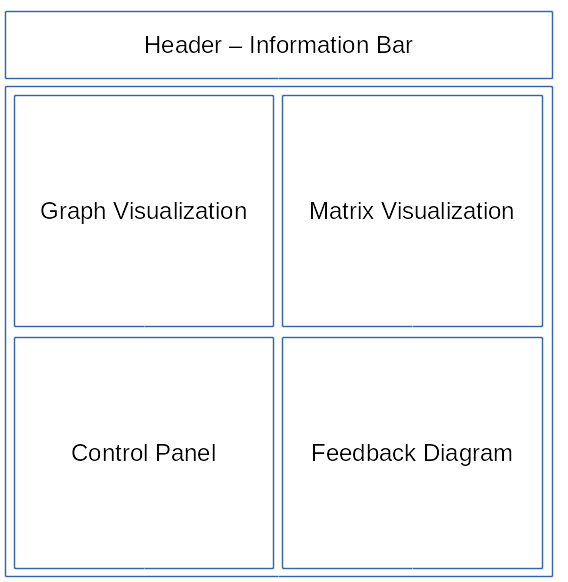
\includegraphics[width=0.44\textwidth]{explain-vis.png}
\hfill
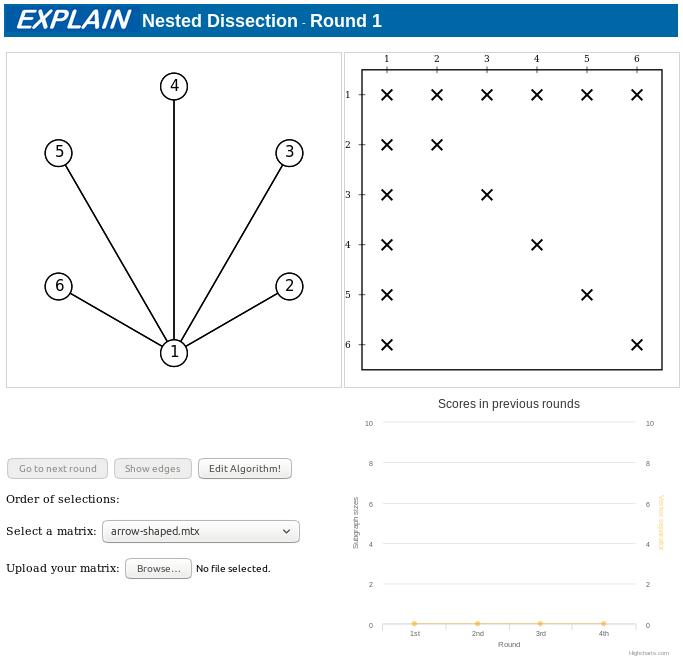
\includegraphics[width=0.48\textwidth]{explain2-init.png}
\caption{
(Left)~\mbox{EXPLAIN} has a fixed layout consists of four sections and a header.
(Right)~An example of the actual implemented view of \mbox{EXPLAIN}.}
\label{explain-design}
\end{figure}
%%%%%%%%%%%%%%%%%%%%%%%%%%%%%%%%%%%%%%%%%%%%%%%%%%%%%%%%%%%%%%%%%%%%%%%%%%%%%%%%%%%%%

We define a set of predefined colors which can be selected by
the corresponding numbers, for example
$\{1=\text{green}, 2=\text{turquoise}, 3=\text{orange}, 4=\text{violet},
5=\text{red}, 6=\text{yellow}, ...\}$.
These colors are selected such that they look perceptually distinct.
However, a user can define any new color by a function that specifies an \textbf{rgb} value.
Another aspect of the design is to use the same colors in graph and matrix view
as well as in the feedback diagram.
This consistent use of colors in the graph
view, the matrix view, and in the feedback diagram makes it easier for the student to understand
the algorithm. We will see examples of this aspect in the different modules
which we explain in \secref{s.av.modules}.


%%%%%%%%%%%%%%%%%%%%%%%%%%%%%%%%%%%%%%%%%%%%%%%%%%%%%%%%%%%%%%%%%%%%%%%%%%%%%%%%%%%%%
\section{Gamification}
\label{s.game}
%%%%%%%%%%%%%%%%%%%%%%%%%%%%%%%%%%%%%%%%%%%%%%%%%%%%%%%%%%%%%%%%%%%%%%%%%%%%%%%%%%%%%
To engage the students more in the teaching process, we improved EXPLAIN such that the students get
more feedback from the software. 
This concept is called gamification~\cite{deterding2011:gug,deterding2011}.
The use of elements from game design in the context of
computer science education is not new. In particular, programming assignments can involve
implementations of games. In \cite{la2007:gfa}, for instance, an introductory programming course is
taught under the common umbrella of two-dimensional game development. Similarly, a game project is
used in a course on software architecture~\cite{Wang2011:EEU}. Programming assignment can also
involve pieces of software that act as a player in an existing game. Rather than implementing a game, we are
interested in situations where students learn by playing a game. 
A publication addressing this aspect of gamification is given in
\cite{Hakulinen2011:usg} where game-based learning is used to teach a course in data structures and
algorithms. A collaborative game is described in \cite{shl:bsc} that aims at improving the teaching
quality of a course on mathematical logic.

The gamification of \mbox{EXPLAIN} is based on finding a solution to a combinatorial scientific problem.
We interpret each solution to a problem instance as a \textit{round}.
The feedback diagram reports the results of previous rounds.
The idea of gamification is used to solve a combinatorial
minimization problem. For example, the gamification in the nested dissection ordering 
consists of minimizing the size of the vertex separator while, at the same
time, balancing the sizes of the remaining components.


\section{Available modules}
\label{s.av.modules}
%%%%%%%%%%%%%%%%%%%%%%%%%%%%%%%%%%%%%%%%%%%%%%%%%%%%%%%%%%%%%%%%%%%%%%%%%%%%%%%%%%%%%
In \mbox{EXPLAIN}, we have already implemented several modules.
After discussing the module for the full one-sided Jacobian compression using the column-intersection graph model,
we explain the modules for the full and partial two-sided Jacobian computation. 
Then, two other modules of nested dissection ordering and parallel matrix-vector
are presented to see other features of the software.
%%%%%%%%%%%%%%%%%%%%%%%%%%%%%%%%%%%%%%%%%%%%%%%%%%%%%%%%%%%%%%%%%%%%%%%%%%%%%%%%%%%%%
\subsection{Column compression}
\label{s.column-compression}
%%%%%%%%%%%%%%%%%%%%%%%%%%%%%%%%%%%%%%%%%%%%%%%%%%%%%%%%%%%%%%%%%%%%%%%%%%%%%%%%%%%%%
In \cite{2013:05,2014:01}, we presented a module of \mbox{EXPLAIN} which visualizes the
coloring algorithm for the column compression interactively.
\figurename~\ref{fig1} shows a screenshot of the column compression module. 
The matrix and the corresponding column intersection graph are visualized beside each other.
In the bottom of the page, different preloaded matrices can be selected 
or a new matrix can be uploaded from a file on the file system of the student's computer. 
The tool provides an interactive interface for the student who can control the algorithm
such as returning to previous steps or loading different graphs and matrices. 
Selecting the vertices in different orderings generates different colorings corresponding to different column compressions.

\begin{figure}
\centering
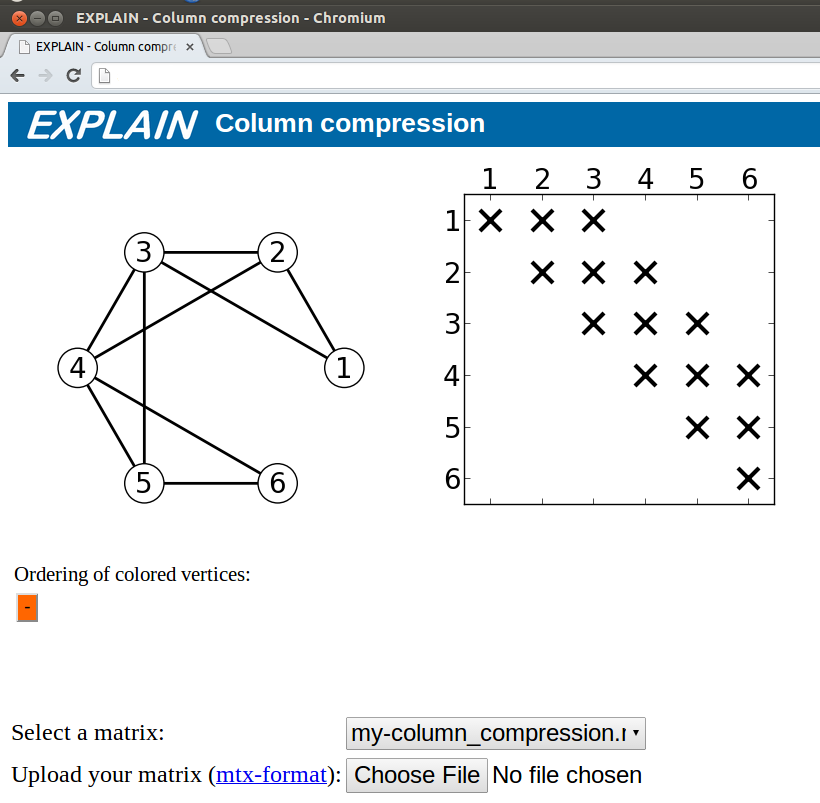
\includegraphics[width=0.5\textwidth]{fig1.png}
\caption{The initial layout of EXPLAIN for some given column compression problem.}
\label{fig1}
\end{figure}
The module allows to select and, thus, color the vertices of a given graph step by step. The order in which the vertices are colored is interactively selected by the student. In each step, when the student selects a vertex, the program checks all of its neighbors regarding the colors. A color of the current step is then greedily selected from the predefined list of colors such that it differs from the colors of those neighbors that are already colored. Recall that a group of columns corresponds to a set of vertices in the graph with the same color. To indicate this, we do not color only the vertices in the graph but also the corresponding columns in the matrix.

Suppose a vertex is selected in the first step. 
This vertex is then colored using the first color of the predefined list. 
Continuing the process of vertex selection, 
different colors are chosen and an ordered list of vertices is created 
which is indicated in the subfigures of \figref{algorihtm} marked by ''Ordering of colored vertices.'' 
Each button of this list is clickable, causing \mbox{EXPLAIN} to return to that step of the algorithm. 
The process continues until all vertices are colored. 
The button labeled by the minus sign will go back to the first step.


\begin{figure}
\centering
\subfigure[Student selected $v_2$ and $v_6$ in that order.]{
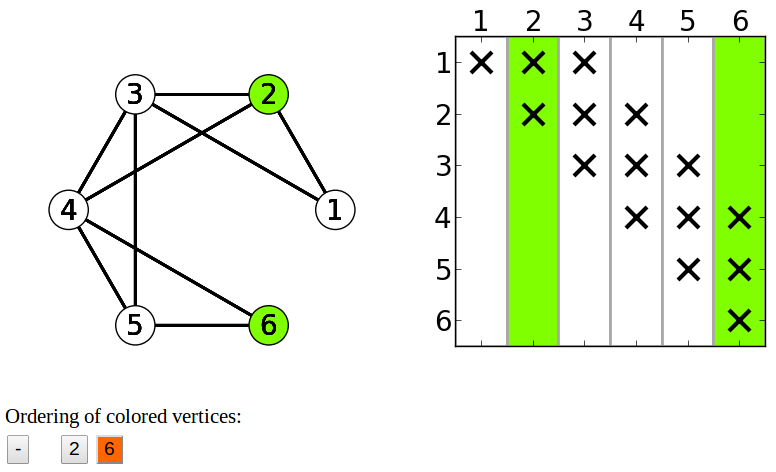
\includegraphics[width=0.47\textwidth]{fig2.png}
\label{fig2}
}
\centering
\subfigure[Student selected $v_2$, $v_6$, $v_3$, $v_5$, $v_1$, and $v_4$ in that order.]{
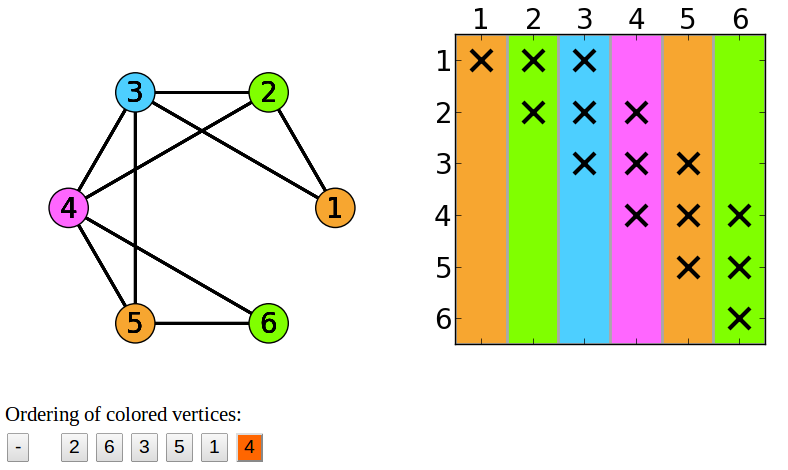
\includegraphics[width=0.47\textwidth]{fig3.png}
\label{fig3}
}
\centering
\subfigure[Student selected vertices as in \figurename~\protect\ref{fig3} and then jumped back to $v_2$.]{
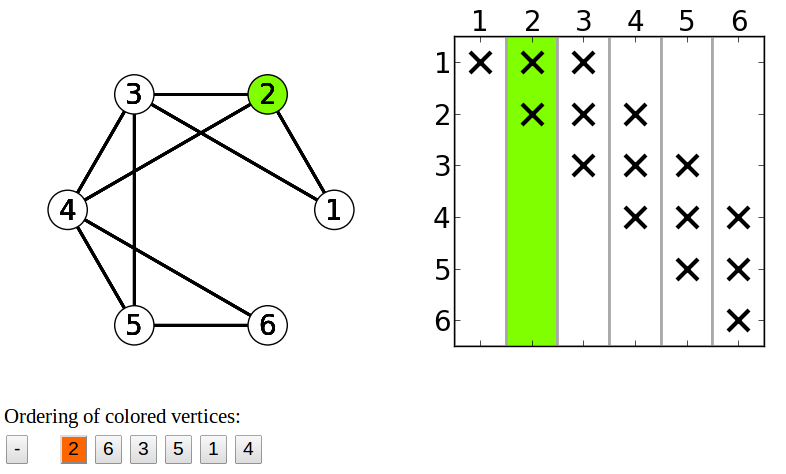
\includegraphics[width=0.47\textwidth]{fig4.png}
\label{fig4}
}
\centering
\subfigure[Student selected $v_2$, $v_1$, $v_3$, $v_4$, $v_5$, and $v_6$ in that order.]{
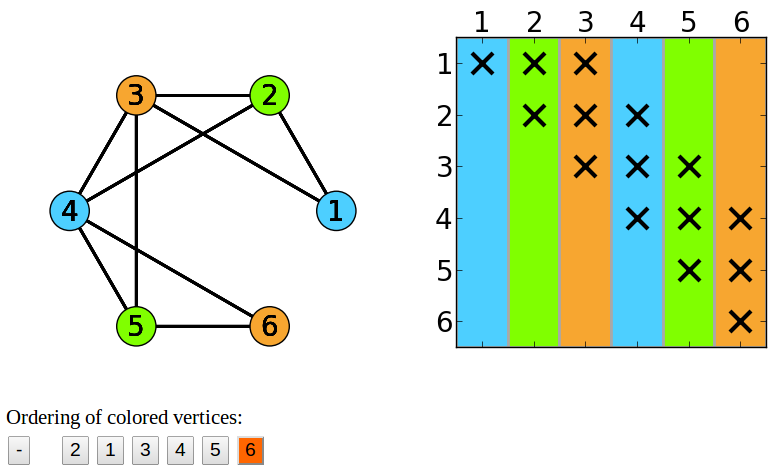
\includegraphics[width=0.47\textwidth]{fig5.png}
\label{fig5}
}
\caption{Display of various situations after interactively choosing vertices.}
\label{algorihtm}
\end{figure}
\figref{fig2} shows a representation of a nonzero pattern of the possible following matrix
\begin{equation}
\label{e:matrixJ}
J =
\begin{bmatrix}
1 & 2 & 3 & 0 & 0 & 0 \\
0 & 4 & 5 & 6 & 0 & 0 \\
0 & 0 & 7 & 8 & 9 & 0\\
0 & 0 & 0 & 10 & 11 & 12\\
0 & 0 & 0 & 0 & 13 & 14 \\
0 & 0 & 0 & 0 & 0 & 15
\end{bmatrix},
\end{equation}
and the related column-intersection graph in which the student has already selected the two vertices $v_2$ and $v_6$. Both vertices are colored with the same since they are not connected by an edge. \figref{fig3} represents the final step which shows that four colors are needed when the vertices are selected in the order $(v_2, v_6, v_3, v_5, v_1, v_4)$ displayed in the vertex list. The group of columns with the same color is compressed to a single column in the seed matrix as follows,
\begin{equation}
\label{e:matrixS}
J \cdot S =
J \cdot
\begin{bmatrix}
 0  & 0 & 1 & 0 \\
 1  & 0 & 0 & 0 \\
 0  & 1 & 0 & 0 \\
 0  & 0 & 0 & 1 \\
 0  & 0 & 1 & 0 \\
 1  & 0 & 0 & 0
\end{bmatrix}
=
\begin{bmatrix}
2 & 3 & 1 & 0 \\
4 & 5 & 0 & 6 \\
0 & 7 & 9 & 8 \\
12 & 0 & 11 & 10\\
14 & 0 & 13 & 0 \\
15 & 0 & 0 & 0
\end{bmatrix}.
\end{equation}
Furthermore, the coloring of \figurename~\ref{fig3} is the one corresponding to that compressed Jacobian~\eqref{e:matrixS}.

Since we want to provide the possibility to return to some step of the algorithm, a history of the selection process is kept in the ordered vertex list. Now, suppose the student selects to return to the step $1$ where the vertex $v_2$ was selected, then the program returns to that step of the algorithm. The resulting state is depicted in \figref{fig4}. Notice that the program keeps the whole history and the student can click on any other buttons in the history list.

On the other hand, the student can select a completely new selection order from the current step which can generate a smaller or larger number of colors. Employing the different ordering $(v_2,v_1,v_3,v_4,v_5,v_6)$ shown in \figurename~\ref{fig5} leads to a reduction of one color compared to the first ordering given in \figurename~\ref{fig3}. In fact, this is the minimum number of colors needed to color this graph. The corresponding seed matrix is given by
$$
S =
\begin{pmatrix}
1 & 0 & 0 \\
0 & 1 & 0 \\
0 & 0 & 1 \\
1 & 0 & 0 \\
0 & 1 & 0 \\
0 & 0 & 1 \\
\end{pmatrix}.
$$
%%%%%%%%%%%%%%%%%%%%%%%%%%%%%%%%%%%%%%%%%%%%%%%%%%%%%%%%%%%%%%%%%%%%%%%%%%%%%%%%%%%%%
\subsection{Full and partial Jacobian computation}%Bidirectional compression}
\label{s.bidirectional}
%%%%%%%%%%%%%%%%%%%%%%%%%%%%%%%%%%%%%%%%%%%%%%%%%%%%%%%%%%%%%%%%%%%%%%%%%%%%%%%%%%%%%
In our publication~\cite{2014:09}, we design and implement an interactive module to
teach bidirectional compression and its connection to star bicoloring.
Figure~\ref{f.explain} shows an overview of the layout of the new module whose top and
bottom part are shown in~(a) and~(b), respectively. In the top part, a graph and a matrix
are visualized next to each other. Here, a matrix with a sparsity pattern in the form of
an arrow is taken as an example. The nonzero pattern of the matrix is shown right and the
corresponding bipartite graph is depicted left. A vertex $r_i$, which is placed on the
left part of the graph, represents the $i$th row of the matrix. Likewise, a vertex on the
right part of the graph labeled $c_i$ corresponds to the $i$th column of the matrix.

%------------------------------------------------------------------------------------------------
\begin{figure}
\centering
\subfigure[]{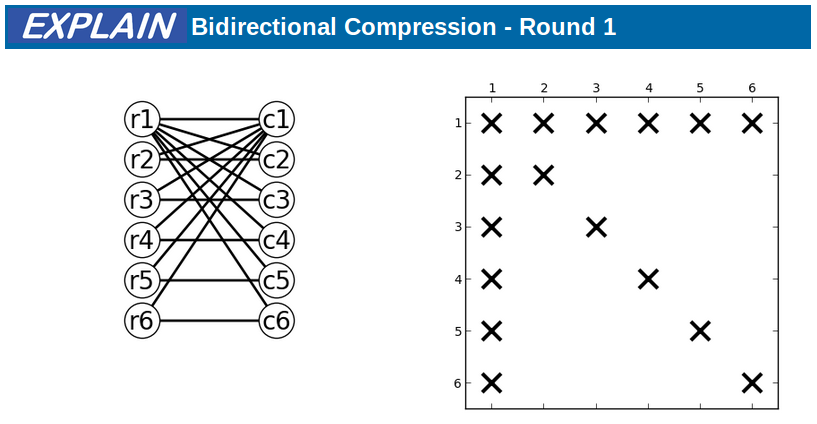
\includegraphics[width=0.43\textwidth]{init-bipartite}}
\hfill
\subfigure[]{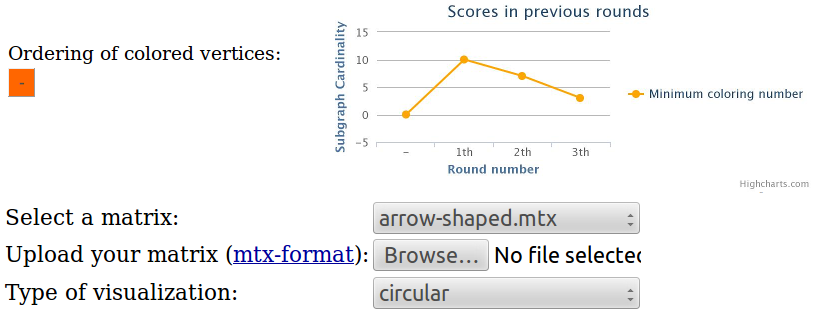
\includegraphics[width=0.55\textwidth]{explain_bottom}}
\caption{The general layout of the bidirectional compression module. (a) The top part
contains the visualization of the graph and its corresponding matrix. (b)
The bottom part contains the intermediate steps, the input, and the
history of selections.}
\label{f.explain}
\end{figure}
%------------------------------------------------------------------------------------------------


%------------------------------------------------------------------------------------------------
\begin{figure}
\centering
\subfigure[]{%
% Matrix C: after choosing 2 vertices
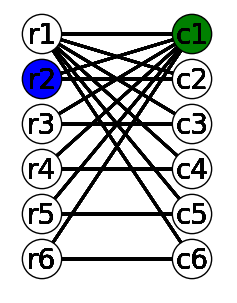
\includegraphics[width=0.18\textwidth]{arrow-shaped-bipartite-graph-twoselected}
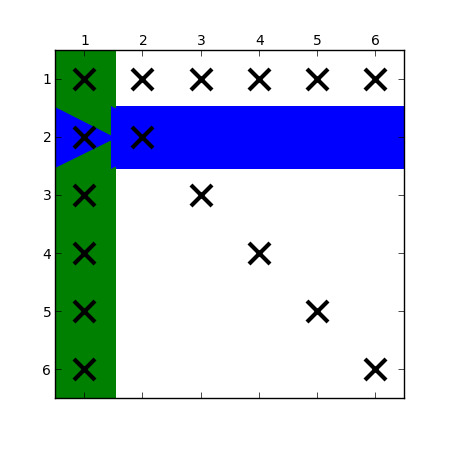
\includegraphics[width=0.26\textwidth]{arrow-shaped-matrix-twoselected}
}
\hfill
\subfigure[]{%
% Matrix C: after having completed the solution process
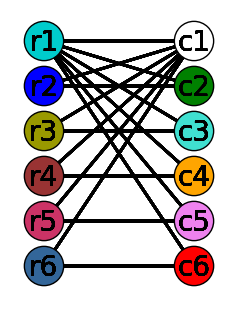
\includegraphics[width=0.18\textwidth]{arrow-shaped-almost-worst-coloring-graph}
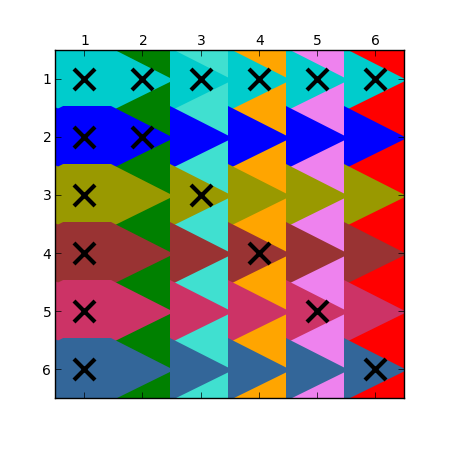
\includegraphics[width=0.26\textwidth]{arrow-shaped-almost-worst-coloring-matrix}
}%
\caption{The graph and the nonzero pattern (a) taken from Fig.~\protect\ref{f.explain}
after the student interactively selected the vertices $r_2$
and $c_1$. A star bicoloring (b) of that example after trying to solve
\MinStaBic\ interactively. This star bicoloring uses $11$ colors.}
\label{f.arrow-shaped2}
\end{figure}
%------------------------------------------------------------------------------------------------

Using any web browser, the student can interactively solve Problem~\ref{p.coloring}, \MinStaBic,
by clicking on
vertices of the bipartite graph. The selection of a vertex by a click refers to choosing
this vertex to be colored next. This coloring is visualized simultaneously in the graph
as well as in the matrix where the neutral color is the color white. By clicking on a row
vertex, the vertex itself and the corresponding row is colored. This color should obey
the rules specified in the definition of a star bicoloring. By clicking on a column
vertex, this vertex and the corresponding column are colored. Recall that a nonzero
element may be in both a colored column as well as in a colored row. In this case, we
divide the square surrounding this element into a triangle and the remaining part. The
triangle part is colored with the row color and the remaining part of the rectangle with
the column color.

%------------------------------------------------------------------------------------------------
\begin{figure}
\centering
\subfigure[]{%
% Matrix C: Minimal number of colors
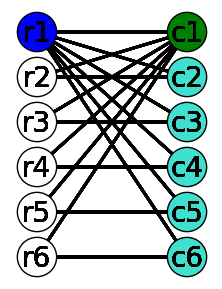
\includegraphics[width=0.18\textwidth]{arrow-shaped-best-coloring-graph}
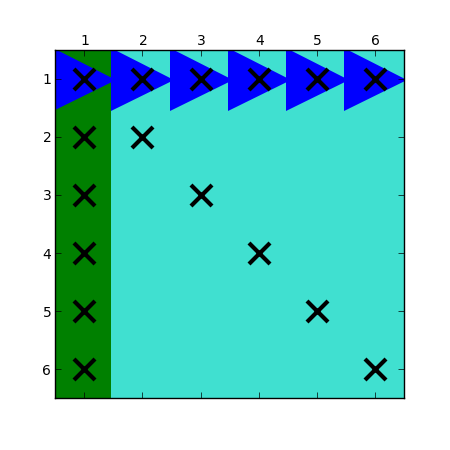
\includegraphics[width=0.26\textwidth]{arrowshaped-best-coloring-matrix}
}%
\hfill
\subfigure[]{%
% A different matrix : after having completed the solution process
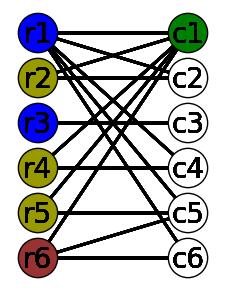
\includegraphics[width=0.18\textwidth]{arrow-shaped2-best-coloring-graph}
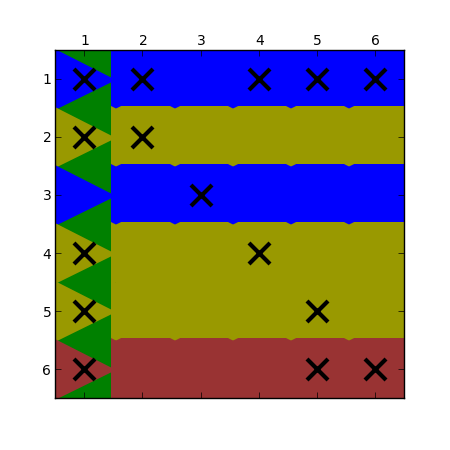
\includegraphics[width=0.26\textwidth]{arrow-shaped2-best-coloring-matrix}
}%
\caption{A star bicoloring (a) of the problem instance from
Fig.~\protect\ref{f.explain} also considered in Fig.~\protect\ref{f.arrow-shaped2}. This
star bicoloring uses $3$ colors and is an exact solution of \MinStaBic. A star bicoloring
(b) of a different problem instance using $4$ colors which is also an exact
solution of \MinStaBic} \label{f.arrow-shaped4}
\end{figure}
%------------------------------------------------------------------------------------------------

We now take the problem with the arrow-shaped nonzero pattern from Fig.~\ref{f.explain}
as an example. Here and in the following, we zoom into the graph and matrix view of the
layout. The student interactively selects a sequence of row and column vertices to solve
\MinStaBic. Figure \ref{f.arrow-shaped2} (a) shows the situation after the student
selected the vertices $r_2$ and $c_1$.
The interactive selection then goes back and forth until a correct star bicoloring is
found. Recall, the process of computing a solution of \MinStaBic\ is called a round.
The current round number is displayed at the top of the web page; see
Fig.~\ref{f.explain}~(a). When a coloring is found at round number $x$, the page shows
the message ``Round $x$ is completed!''

Selecting vertices in different orders will typically result in different star
bicolorings. A star bicoloring which is interactively chosen will not always have a
minimal number of colors. For example, the order of vertex selection visualized in
Fig.~\ref{f.arrow-shaped2}~(b) leads to a star bicoloring using $11$ colors, which is
obviously not the minimal number of colors. Here, all columns and rows are colored
differently. In contrast, Fig.~\ref{f.arrow-shaped4}~(a) illustrates an exact solution of
\MinStaBic\ for this problem instance using the minimal number of $3$ colors.

After completing a round, the student can solve the same problem instance once more. In
this case, the round number will be incremented, the colors will be removed, and another
round is started using the initial situation depicted in Fig.~\ref{f.explain}~(a). The
history of the number of non-neutral colors used in previous rounds is displayed below
the matrix in a score diagram as shown in Fig~\ref{f.explain}~(b).

The subtle issues in understanding the connection between bidirectional compression and
star bicoloring are more lucid when considering more irregularly-structured nonzero
patterns. Another problem instance with a different nonzero pattern is shown in
Fig.~\ref{f.arrow-shaped4}~(b). Here, it is more difficult to find out that this star
bicoloring with $4$ colors is indeed an exact solution to \MinStaBic.

%\subsection{Partial Jacobian computation}
We extend this module to support
the partial Jacobian computation. Here, the student should
first select the required elements which are edges in Bipartite graphs.
So, when the student clicks on an edge, the color of this edge
as well as the color of the corresponding nonzero element will be changed to red.
These selected edges and nonzero elements are added to the required elements
as shown in Figure~\ref{partial_coloring_bad_coloring}.

As soon as the student starts to click the vertices, the required elements
become fixed, i.e., no new required element can be added.
The process of coloring is completely like the previous module.
Figure~\ref{partial_coloring_good_coloring} (a) shows a selection in which 
the student selects only column vertices. The result is a star bicoloring
restricted to red edges with $4$ colors.
A coloring with a smaller number of colors 
is shown in Figure~\ref{partial_coloring_good_coloring} (b)
in which a row vertex is selected first.

\begin{figure}
\centering
\subfigure[]{
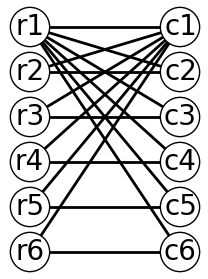
\includegraphics[width=0.18\textwidth]{arrow_shaped_partial_coloring_oneselect_graph}
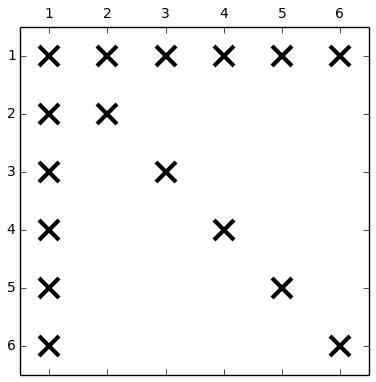
\includegraphics[width=0.26\textwidth]{arrow_shaped_partial_coloring_oneselect_matrix}}
\hfill
\subfigure[]{
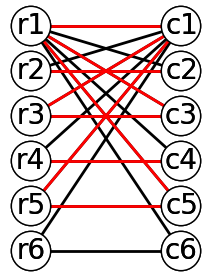
\includegraphics[width=0.18\textwidth]{arrow_shaped_partial_coloring_init_graph}
\includegraphics[width=0.26\textwidth]{arrow_shaped_partial_coloring_init_matrix}}
\caption{
(a) The initial view of the module when no required edges are selected.
(b) The user selects first the required edges. These required edges and the corresponding
nonzero elements get the red color.}
\label{partial_coloring_bad_coloring}
\end{figure}

\begin{figure}
\centering
\subfigure[]{
\includegraphics[width=0.18\textwidth]{arrow_shaped_partial_coloring_init_graph_bad_coloring}
\includegraphics[width=0.26\textwidth]{arrow_shaped_partial_coloring_init_matrix_bad_coloring}}
\hfill
\subfigure[]{
\includegraphics[width=0.18\textwidth]{arrow_shaped_partial_coloring_init_graph_good_coloring}
\includegraphics[width=0.26\textwidth]{arrow_shaped_partial_coloring_init_matrix_good_coloring}}
\caption{
(a) A graph coloring with four colors in which only column vertices are selected.
(b) A graph coloring with three colors in which the user colors a row vertex first.}
\label{partial_coloring_good_coloring}
\end{figure}

\subsection{Nested dissection ordering}
In our paper~\cite{2014:02}, we present the nested dissection module to
illustrate the connection between the following scientific computing and combinatorial problems,
\begin{problem}[Nested Dissection Ordering]
\label{p.nest.dissect}
Given a sparse symmetric positive
definite matrix $A$, find a symmetric permutation $P^T A P$ of~$A$ in the form of 
\begin{equation}
\label{e.A}
A^{\prime} =
\begin{bmatrix}
A_1 & 0   & B_1^T \\[0.2em]
0   & A_2 & B_2^T \\[0.2em]
B_1 & B_2 & C
\end{bmatrix} ,
\end{equation}
such that the size of the block~$C$ is minimized while the sizes of the blocks $A_1$ and $A_2$ are
balanced.

\end{problem}
\begin{problem}[Small Vertex Separator]
\label{p.small.ver.sep} Given the graph $G$ associated with a sparse
matrix $A$, find a disjoint decomposition of the vertices $V = V_1 \cup V_2 \cup S$ with a vertex
separator $S$ such that the size of the vertex separator, $|S|$, is minimized while the sizes of
the two remaining components, $|V_1|$ and $|V_2|$, are balanced.
\end{problem}

The graph model of this problem has the simple graph layout considering the matrix
as the adjacency matrix of a graph.
The algorithm from~\cite{2014:02} searches for a so-called vertex-separator set
corresponding to the block $C$ here. A vertex separator $S$ of the given graph $G$
is a subgraph of $G$ if removing $S$ and its adjacent edges from $G$ results in two
disconnected components $V_1$ and $V_2$ of $G$.
Suppose we move rows and columns corresponding to the vertex separator to the end of
the matrix and bringing together
the corresponding columns of $V_1$ and $V_2$ by a permutation,
then a nested dissection would be visualized on the matrix.

In this module representing a bisection, a round consists of finding a vertex separator.
Figure~\ref{initial_10} shows the initial layout of an example
and the selection of the vertex $v_10$ for the set of vertex separator. 
The module moves the
column corresponding to the selected vertex to the end of the matrix
and both the vertex and its corresponding column get the orange color.
Additionally, the adjacent edges of the vertex are removed for a better visualization
(compare \figref{initial_10} (a) and \figref{initial_10} (b)).

\begin{figure}
\centering
\subfigure[]{
\includegraphics[width=0.23\textwidth]{graph_initial}
\includegraphics[width=0.23\textwidth]{matrix_initial}}
\hfill
\subfigure[]{
\includegraphics[width=0.23\textwidth]{graph_10_selected}
\includegraphics[width=0.23\textwidth]{matrix_10_selected}}
\caption{
(a) Two equivalent representations in terms of a graph and a matrix.
(b) Graph and matrix view after selecting the vertex number~10.
The decomposition into two blocks is still not shown as the graph is not yet
decomposed into two disconnected components.}
\label{initial_10}
\end{figure}

Figure~\ref{selected_4_10_8_10} shows two scenarios.
We have an unbalanced result in~\figref{selected_4_10_8_10}(a)
in which the vertex $v_4$ is selected after the initial selection of $v_10$.
However, \figref{selected_4_10_8_10}(b) results in a balanced result
by only selecting $v_8$ instead of $v_4$.
When a vertex separator is found, 
the software performs the permutation 
and colors the two disconnected components of graph
as well as the distinct block on diagonals with blue and red.

\begin{figure}
\centering
\subfigure[]{
\label{selected410}
\includegraphics[width=0.23\textwidth]{graph_4_10_selected}
\includegraphics[width=0.23\textwidth]{matrix_4_10_selected}}
\hfill
\subfigure[]{
\label{selected810}
\includegraphics[width=0.23\textwidth]{graph_8_10_selected}
\includegraphics[width=0.23\textwidth]{matrix_8_10_selected}}
\caption{
(a) Graph and matrix view after selecting the vertices number 10 and then 4.
The selection is not adequate as the sizes of blocks are not balanced.
(b) Graph and matrix view after selecting the vertices number 10 and then 8. The block sizes are balanced and the separator size is minimized.}
\label{selected_4_10_8_10}
\end{figure}

The feedback diagram from different rounds looks
like \figref{diagram}. Here, the blue and red curves should have
values close to each other since this indicates the balancing condition.
The orange curve should be as small as possible
because it represents the minimization of the separator size.
In in the last round of this figure, we see a balanced result with minimal separator size.
\begin{figure}
\centering
\includegraphics[width=0.47\textwidth]{diagram}
\caption{Score diagram resulting from four different rounds.}
\label{diagram}
\end{figure}

Based on the new features of \mbox{EXPLAIN 2.0}, we update the previous
bisection to a recursive bisection algorithm.
It contains the bisection itself. So, the student selects the vertex separator
as before until the graph becomes disconnected.
In this new version, the vertex separator is shown in orange on the bottom
of the graph. Also the two remaining components of the graph are shown separately
in two different colored circles at the top of this figure.
In Figure~\ref{bad_bisection}, the result of a selection is visualized which
is not balanced.
Figure~\ref{good_bisection} also shows the results of a balanced selection.

\begin{figure}
\centering
\includegraphics[width=0.8\textwidth]{bad_bisection}
\caption{A selection results in an unbalanced bisection of graph.}
\label{bad_bisection}
\end{figure}

\begin{figure}
\centering
\includegraphics[width=0.8\textwidth]{good_bisection}
\caption{A selection results in a balanced bisection of graph.}
\label{good_bisection}
\end{figure}

\begin{figure}
\centering
\includegraphics[width=0.8\textwidth]{bad_disection}
\caption{A complete nested dissection with an unbalanced result.}
\label{bad_disection}
\end{figure}


\begin{figure}
\centering
\includegraphics[width=0.8\textwidth]{good_disection}
\caption{A complete nested dissection with a balanced result.}
\label{good_disection}
\end{figure}

\begin{figure}
\centering
\includegraphics[width=0.8\textwidth]{good_disection2}
\caption{A complete nested dissection with an even more balanced result.}
\label{good_disection2}
\end{figure}

Now, in contrast to the previous version, the student can click further
on the vertices of each component. This selection would trigger a recursive
bisection of two components of matrix as well. Again, this selection goes forward until
both graph components become disconnected. The vertex separators
are moved to the bottom of the graph components as well as the graph components
are shown separately.
Figure~\ref{bad_disection} and Figure~\ref{good_disection} 
illustrate two unbalanced and balanced results of nested dissection,
respectively. Figure~\ref{good_disection2} shows how the results can
get even more balanced.

The corresponding feedback diagram is modified such that
both the size of vertex separator as well as the size of four graph components
can be visualized. In this diagram, the separator size shows the sum of all
the vertex separators of all recursion levels.
Figure~\ref{barchart} shows a possible selection history.
The line chart shows the size history of the vertex separator
and four bar chart grouped together shows the size history of the graph parts.
The colors are also the same colors used in the graph and matrix visualizations.
The goal here is to minimize the size of vertex separator as well as balancing the
size of subgraphs. We achieved a balanced results in the fourth round of selection.
\begin{figure}
\centering
\includegraphics[width=0.6\textwidth]{chart2}
\caption{The size of four subgraphs, shown as bar charts,
resulted from nested dissection compared in different rounds.
The color of bar charts are related to the colors of corresponding subgraph.
The curve of the orange color is also the size of vertex separator.}
\label{barchart}
\end{figure}

%%%%%%%%%%%%%%%%%%%%%%%%%%%%%%%%%%%%%%%%%%%%%%%%%%%%%%%%%%%%%%%%%%%%%%%%%%%%%%%%%%%%%%%%%%%%%%%%
\clearpage
\subsection{Parallel matrix-vector product}
%%%%%%%%%%%%%%%%%%%%%%%%%%%%%%%%%%%%%%%%%%%%%%%%%%%%%%%%%%%%%%%%%%%%%%%%%%%%%%%%%%%%%%%%%%%%%%%%
In our paper~\cite{2015:3}, we present a module for a parallel matrix-vector
product to illustrate the connection between the following scientific computing and combinatorial problems.
\begin{problem}[Scientific Computing Problem]
\label{p.par.mat.vec}
Given a large sparse matrix $A$ with a symmetric nonzero pattern and a dense
vector $x$. Suppose we want to compute the sparse matrix-vector product
$y \leftarrow Ax$ on a computer with distributed memory. Find a non-redundant
data distribution of the nonzero elements of $A$ in a row-wise fashion and a
consistent distribution of $x$ and $y$ such that the communication between
processes is minimized while the number of arithmetic operations is balanced
between the processors.
\end{problem}
\begin{problem}[Combinatorial Problem]
\label{p.par.mat.vec.graph}
Given an undirected connected graph $G$, find a partition of the vertices $V$ into
nonempty disjoint subsets such that the number of edges with incident vertices
in different partitions is minimized while the number of vertices of the subsets
is balanced.
\end{problem}
These two products are connected by letting a row $i$ of $A$ be represented by a vertex $v_i$
in $G$ and the nonzero elements in the positions $(i,j)$ and $(j,i)$ correspond to
an edge between vertices $v_i$ and $v_j$.
Let $P: V \rightarrow \{1, 2, \dots, p\}$ be the vertex partition to $p$ processes
that decomposes the set of nodes $V$ of the graph into~$p$ subsets $V_1$, $V_2$, \dots,
$V_p$ such that
$$
V = V_1 \cup V_2 \cup \dots \cup V_p
$$
with $V_i \cap V_j = \emptyset$ for~$i \neq j$. This decomposition of $V$ represents 
the distribution of the rows of $A$ to $p$ processes.

Assuming that the number of nonzeros is roughly the same for each row of $A$, the
computation is evenly balanced among the $p$ processes if the partition $P$ is
$\varepsilon$-balanced defined as
\begin{equation}\label{e.bal}
\max_{1 \leq i \leq p} |V_i| \leq (1 + \varepsilon) \frac{|V|}{p} ,
\end{equation}
for some given $\varepsilon > 0$. The graph partitioning problem consists of minimizing
the number of edges with incident vertices in different partitions (the so-called cut size) 
of an $\varepsilon$-balanced partition. It is a hard combinatorial problem~\cite{gj:com}.


The parameter $\varepsilon$ introduced in~\eqref{e.bal} is used to quantify the degree of
imbalance allowed in a data distribution. If $\varepsilon = 0$ all processes are assigned
exactly $|V|/p$ rows of $A$, meaning that no imbalance is allowed at all. When
increasing $\varepsilon$ the load balancing condition~\eqref{e.bal} is relaxed. The
larger $\varepsilon$ is chosen, the larger is the allowed imbalance. Thus, in some way,
$\varepsilon$ quantifies the deviation from a perfect load balance. An equivalent form
of~\eqref{e.bal} is given by
\begin{equation}\label{e.bound}
\frac{p}{|V|} \max_{1 \leq i \leq p} |V_i| - 1 \leq \varepsilon ,
\end{equation}
which can be interpreted as follows. Suppose that you are not looking for an
$\varepsilon$-balanced partition $P$ for a given $\varepsilon$, but rather turn this
procedure around and ask: ``Given a partition $P$, how large need $\varepsilon$ at least
be so that this partition is $\varepsilon$-balanced?'' Then the left-hand side of the
inequality~\eqref{e.bound} which we call \emph{deviation bound} gives an answer to that
question. The extreme cases for the deviation bound are given by $0$ if the distribution is
perfectly balanced and $p-1$ if there is one process that gets all the data. 

Figure~\ref{f.explain.matvec} shows the overall layout of this interactive
module for sparse matrix-vector multiplication.
The top of this figure visualizes 
the representation of the problem regarding the graph~$G$ as well as in terms
of the matrix $A$ and the vector $x$. Below on the left, there is a panel of
colors representing different processes and another panel displaying the order of
selecting vertices of the graph. Next, on the right, there is a feedback diagram recording
values characterizing communication and load balancing.

%------------------------------------------------------------------------------------------
% Overall Layout of Module
\begin{figure}
\centering
\includegraphics[width=0.7\textwidth]{final}
\caption{Overall structure of the sparse matrix-vector multiplication module.}
\label{f.explain.matvec}
\end{figure}
%------------------------------------------------------------------------------------------

This figure gives an overall impression of the status of the module after a data
distribution is completed. Here, $p=4$ processes represented by the colors blue, green,
red, and yellow get data by interactive actions taken by the student.
Figure~\ref{f.beginning} now shows the status of the module in a phase that is more
related to the beginning of that interactive procedure. For a given matrix, the student
can distribute the data to the processes by first clicking on a color and then clicking
on an arbitrary number of vertices. That is, the distribution of vertices to a single
process is determined by first clicking on a color $j$ and then clicking on a particular
number of vertices such that these vertices are distributed to the process $j$.
Then, by clicking on the next color, this procedure can be repeated until
all vertices are interactively colored and, thus, the data distribution $P$ is finally
determined.

Figure~\ref{f.beginning} illustrates the situation after the student distributed
vertices~$\{ v_1, v_2, v_3 \}$ to the blue process
and the vertices~$\{ v_7, v_8, v_{10}\}$ to the green
process. By interactively assigning a vertex to a process, not only the vertex is colored
by the color representing this process, but also the row in the matrix as well as the
corresponding vector entry of $x$ are simultaneously colored with the same color.
This way, the data distribution is visualized in the graph and the matrix
simultaneously which emphasizes the connection between the matrix representation and the
graph representation of that problem. By inspection of that panel
in~\figref{f.explain.matvec}, we find out that the status depicted in \figref{f.beginning} is an
intermediate step of the interactive session that led to the data distribution
in~\figref{f.explain.matvec}. Any box labeled with the number of the chosen vertex in that panel
is also clickable allowing the student to return to any intermediate state and start a
rearrangement of the data distribution from that state.

%------------------------------------------------------------------------------------------
% Interactive Selection of Vertices
\begin{figure}
\centering
\includegraphics[width=0.7\textwidth]{twoColors}
\caption{The intermediate state after the student selected six vertices.}
\label{f.beginning}
\end{figure}
%------------------------------------------------------------------------------------------

In this module, the problem consists of distributing all data needed to
compute the matrix-vector product to the processes. Equivalently, the distribution of all
vertices of the corresponding graph to the processes is a round. Suppose that round~2 is
completed in \figref{f.explain.matvec}. Then, the student can explore the data distribution in
more detail by clicking on a color in the panel labeled ``Color of processes.'' Suppose
that the student chooses the red process, then this action will modify the appearance of
the vector $x$ in the matrix representation to the state given
in~\figref{f.communication}. Here, all vector entries that need to be communicated to the
red process are now also colored red. 
The background color in the vector still represents the process
that stores that vector entry. 

%------------------------------------------------------------------------------------------
% Communication structure
\begin{figure}
\centering
\includegraphics[width=0.7\textwidth]{redComm}
\caption{All vector entries $x_i$ to be communicated to the red process are drawn in red.}
\label{f.communication}
\end{figure}
%------------------------------------------------------------------------------------------

After completion of a round, it is also instructive to focus on the quality of the data
distribution $P$. Recall that the graph partitioning problem aims at minimizing the cut
size of~$P$ while balancing the computational load evenly among the processes. 
\figref{f.score} shows the feedback diagram. For each round, this diagram shows the cut size
using the label ``communication volume.''
In that feedback diagram, the student can attempt to minimize the communication volume over some rounds.

%------------------------------------------------------------------------------------------
% Score diagram
\begin{figure}
\centering
\includegraphics[width=0.8\textwidth]{chart}
\caption{The communication volume and the deviation bound versus various rounds.}
\label{f.score}
\end{figure}
%------------------------------------------------------------------------------------------
The feedback diagram shows the value of the deviation bound for each round.
A low deviation bound
indicates a partition that balances the computational load evenly, whereas a large
deviation bound represents a significant imbalance of the load. The score diagram helps the
student to evaluate the quality of a single data distribution and to compare it with
distributions obtained in previous rounds. This feedback to the student is in
the spirit of computer games, where a score has only a low immediate relevance to the
current game. However, the idea is to achieve a ``high score'' and try to motivate the
player to beat that score in subsequent rounds, thus offering an extra challenge. For
this educational module, a ``high score'' would consist of a low communication value
together with a small deviation bound.

%%%%%%%%%%%%%%%%%%%%%%%%%%%%%%%%%%%%%%%%%%%%%%%%%%%%%%%%%%%%%%%%%%%%%%%%%%%%%%%%%%%%%%
\section{New Features in EXPLAIN 2.0}
\label{s.alg.edit}
%%%%%%%%%%%%%%%%%%%%%%%%%%%%%%%%%%%%%%%%%%%%%%%%%%%%%%%%%%%%%%%%%%%%%%%%%%%%%%%%%%%%%%
EXPLAIN 2.0 came with various features which are
discussed in the following paragraphs. 
The new major feature is an algorithm editor.
In EXPLAIN 2.0, the student can see and edit the source code of an algorithm
beside the visualization of the graph and matrix.
There is a new button in the control button named as \textit{Edit Algorithm!}.
Clicking this button shows an editor with the source code of the corresponding module.
This source code is written in a simple scripting language.
Figure~\ref{f.custom_module} illustrates the column compression module.
As it can be seen, an editor with the corresponding source code of 
the column compression module is shown in the right part of the figure.
Additionally, the student can see an animation of this algorithm
by first selecting and ordering and then clicking the button 
named as \textit{animate}.
An animation goes through the vertices and executes each line of the algorithm
one by one to visualize the algorithm during the time.
The student can stop the algorithm and select the speed of execution.

Figure~\ref{f.bottom_new_explain} shows the control panel of EXPLAIN 2.0 for the 
nested dissection module in the left figure and the column compression
module in the right figure. 
Comparing to EXPLAIN 1.0, we have here three new buttons for the three functionalities:
going to next round, doing a postprocessing, and editing an algorithm.
The first button named as \textit{Go to next round} goes to the next round even if 
the current round is not completed. The second button is for a postprocessing
step. A postprocessing is an action which can be done when a round is completed.
It can be different for each module.
For example, Figure~\ref{f.bottom_new_explain} (Left) has the postprocessing named
as \textit{Show edges}. This shows the edges between the vertex separators
and the subgraphs which we remove during the selection.
Another example is Figure~\ref{f.bottom_new_explain} (Right) which does not have
any postprocessing. So, the button is disabled.
The third button is to show and hide the algorithm editor.
The label of the button is first \textit{Edit Algorithm!}
and changed to \textit{Finish Editing!} after clicking.

Another minor change is the reference to a publication which explains the 
module. Figure~\ref{f.bottom_new_explain} (Left) and (Right) shows the two publications
\cite{2013:05} and \cite{2014:02} for the nested dissection and the column compression module
and the link to the publishers.
%------------------------------------------------------------------------------------------
% Custom Module
\begin{figure}
\centering
\includegraphics[width=\textwidth]{custom_module}
\caption{The code of the corresponding module is visualized beside
graph and matrix. This code is in a simple scripting language.
The user specifies the order and this code is executed based on that order.}
\label{f.custom_module}
\end{figure}
%------------------------------------------------------------------------------------------

%------------------------------------------------------------------------------------------
% Custom Module
\begin{figure}
\centering
\includegraphics[width=0.45\textwidth]{bottom_new_explain1}
\hfill
\includegraphics[width=0.45\textwidth]{bottom_new_explain}
\caption{The control panel of EXPLAIN 2.0 is visualized.
It has three new buttons for going to the next round,
doing a postprocessing step, and editing the algorithm.
Additionally, it has a new reference link to a publication
for this module.
(Left) The control panel is visualized for the nested dissection module.
Here, the postprocessing step is to show the missing edges which we remove
during the selection processes. 
(Right) The control panel is visualized for the column compression module. 
In this module, we do not have any postprocessing step. Hence, the button is disabled.}
\label{f.bottom_new_explain}
\end{figure}
%------------------------------------------------------------------------------------------
\section{Implementation Details}
\label{s.impl.explain}
Lülfesmann~\cite{Lulfesmann2010} first introduced an standalone EXPLAIN needed a client with administrator privileges to install Python libraries as well as the software itself.
Here, we introduce two new releases of EXPLAIN.
\subsection{EXPLAIN 1.0}
\label{s.impl.explain1}
This section is a summary of the implementation details 
of EXPLAIN 1.0 in our publication~\cite{2013:05}.
In EXPLAIN 1.0, the software is moved to the online platform which means the student needs just a web browser to work with the software.
EXPLAIN 1.0 combines several Python packages. More precisely, the graph data structure is handled by \textit{NetworkX} \cite{networkx2008}. It provides different operations like creation and deletion of vertices and edges. It also allows the programmer to access characteristic graph information such as the neighbor vertices and the number of vertices. Using this library together with \textit{matplotlib} \cite{matplotlib2007} covers the different aspects of visualization. This library produces different layouts of graphs as well as the properties of vertices and edges. The matrix manipulation and visualization are handled by \textit{Scipy}~\cite{scipy2001}, specifically the construction and the visual layout of sparse matrices.

The conversion from the standalone to the online version needs the Python library \textit{Mod\_python}~\cite{modpython2013}. It comes from the \textit{Apache} project including the Python interpreter in the given Apache web server. Using this library helps to keep the previous program structure as much as possible.

The library \textit{Mod\_python} assists to implement folder management, user interaction, cookie handling, and the web interface. Specifically, the \textit{Mod\_python} modules like \textit{Apache}, \textit{util}, and \textit{PSession} are used to migrate the previous version of \mbox{EXPLAIN} to a web version. As already mentioned, the Python interpreter is embedded into the web server by the \textit{Mod\_python} module.

In the standalone version, an event was handled by a local Python function but, in the new version, there are two sides: server and client. The web browser at client side shows HTML websites with embedded Javascript source code while the server side is a Python server. Since the buttons are HTML buttons and the events are Javascript functions, a Javascript function submits a form to the server containing the execution request and parameters to the related Python function. Then, the called Python function writes the dynamically generated result as an HTML string to the Apache request. The server sends back the HTML string and the client shows the string as a web
page.

As an example, 
the basic algorithm of coloring in the column compression module and 
keeping the history is shown in the pseudo-codes given in \figurename~\ref{f:alg}. The first procedure represents what happens when a student clicks on a vertex. The second one shows how the history of matrix and graph images are loaded when the student clicks on one of the history buttons.

The first procedure, \textsc{VertexClicked}, takes the selected vertex $v$ as an input parameter. To color this vertex $v$, it finds the first color from the list $ColorList$ that is different from the colors of the neighbors of $v$. The coloring of the graph is then changed, shown, and saved as an image. 
Also, the vertex $v$ is added to the ordered list, $Hist$, of selected vertices for the history.

The second procedure, \textsc{HistClicked}, takes the selected history $h$. This history will be used to find and plot the previously stored images of the matrix and the graph. Also, the variable $IsInHist$ specifies that the program is in the ``history mode'' which is important if the user selects a vertex different from the previous order. In this case, the program overwrites the current history and saves new images.

\begin{figure}
\centering
\begin{algorithmic}[1]
\State $ColorList \gets \{\text{green}, \text{turquoise}, \text{orange}, \text{violet}, ...\}$
\State $Hist \gets \{\}$\Comment{History of selected vertices.}
\State $WhereInHist \gets 0$\Comment{Where in history are we?}
\State $IsInHist \gets False$\Comment{Are we in history mode?}
\State
\Procedure{VertexClicked}{$v$}\Comment{User clicks vertex $v$.}
\State $ns\gets$ neighbors($v$)
\State $ColorIndex \gets 1$\Comment{Allowed color index}
\For{$i \gets 1$ \textbf{to} size$(ColorList)$}
\State $AllowedColor \gets True$
\For{$j \gets 1$ \textbf{to} size$(ns)$}
\If{$ColorList[i] =$ color$(ns[j])$}
\State $AllowedColor \gets False$
\EndIf
\EndFor
\If{$AllowedColor = True$}
\State $ColorIndex \gets i$
\State Break
\EndIf
\EndFor
\State Color $v$ with the color $ColorList[ColorIndex]$
\State
\If{graph and matrix images are not already saved}
\State SaveMatrix()\Comment{Using a specific name}
\State SaveGraph()\Comment{Using a specific name}
\EndIf
\If{$IsInHist = True$}
\For{$i\gets WhereInHist+1$ \textbf{to} size($Hist$)}
\State $Hist.removeElementAtPosition(i)$
\EndFor
\State $Hist$.add($v$)
\State $IsInHist \gets False$
\Else
\State $Hist$.add($v$)
\EndIf
\State Update($Hist$)\Comment Update history buttons
\EndProcedure
\State
\State
\Procedure{HistClicked}{$h$}\Comment{User clicks history $h$.}
\State OpenMatrix($h$)\Comment{Plot/load matrix with specific name}
\State OpenGraph($h$)\Comment{Plot/load graph with specific name}
\State $WhereInHist \gets find(Hist,h)$\Comment{The location of $h$}
\State $IsInHist \gets True$
\EndProcedure
\end{algorithmic}
\caption{Pseudocode of the event handling in EXPLAIN}
\label{f:alg}
\end{figure}


\subsection{EXPLAIN 2.0}
\label{s.impl.explain2}
In EXPLAIN 2.0, we changed the code such that it becomes more efficient and easier to extend.
In the previous version, the module was mainly based on the Python libraries:
\textit{NetworkX} \cite{networkx2008} for the graph data structure,
\textit{matplotlib} \cite{matplotlib2007} for the visualization aspects,
\textit{Scipy}~\cite{scipy2001} for the sparse matrix computation, and
\textit{Mod\_python}~\cite{modpython2013} for the web-based version.

There were two problems with the previous implementation. First, the final visualization
of graph and matrix was always an image.
So, the time for saving and loading the image was always a problem.
Second, since the final result was HTML/JS code and the computation part was in Python,
an overhead of the server management for \textit{Mod\_python} is always added to the system.

In the new implementation, we replace all Python parts with the Javascript code.
We chose the Javascript library D3 (Data-Driven Documents)
because of its power of control and visualization.
We apply the data structure of adjacency list for graph
combined with the object structure of the Javascript. 
Figure~\ref{f.graph-ds} shows an illustration
of this graph data structure. There is an array representing the vertices.
Each cell of array this points to another array \textit{edges} which contains
the identity of the vertices which are neighbors of that vertex.
Here, we show that the data structure contains other properties like colors.
Using the object structure of Javascript,
it can be extended dynamically to include any other properties which may be necessary later. For example, two properties \textit{distance} and \textit{parent} are added
in the implementation of Breadth-First Search (BFS).

%-----------------------------------------------------------------------------------------------
\begin{figure}
\centering
\includegraphics[width=0.38\textwidth]{graph}
\caption{The graph data structure which is implemented in EXPLAIN 2.0.}
\label{f.graph-ds}
\end{figure}
%-----------------------------------------------------------------------------------------------
We consider a model-view-control (MVC) design pattern~\cite{osmani2012learning} for our implementation.
An important aspect of our design is the suitable connection of the
model and view. A practical approach enables the direct change in view while keeps the
separation of the view and model. 
So, we have unique ids for
edges and vertices. The unique ids for vertices are the concatenation of the
string “ver” and the actual id of the vertex. Similarly, the unique ids for edges are
defined as the concatenation of the four strings “edge”, the source vertex, “-“,
and the target vertex. The same idea applies to the matrix view. Each cell of the matrix
is accessible through a unique id combining the strings “cell”, the row index,
"-", and the column index. 
Each nonzero of the matrix also gets the unique id that is built in a similar way
as the cell id, but replacing the string "cell" by the string "nnz".

The previous discussion of the view access enables us to select the
specific element and change its behavior and properties. For example, the following
code changes the color of the vertex with the id~\textit{i} to the red color 
and the color of a matrix cell to the blue color,
\begin{lstlisting}
d3.select("#ver"+i).set_color(red);
d3.select("#cell"+i+"-"+j).set_color(blue);
\end{lstlisting}

Another aspect of the implementation is the order of drawing edges and
vertices. Since we do not want to draw the edges on the top of the vertices,
the edges should be drawn first. On the other hand, we draw an edge
only by getting its vertices positions. This direct connection helps to avoid
the several update of view.
To solve this problem, 
we draw the edges and vertices in order by using the grouping concepts of D3.

After the first design of the software, we then considered the actual interface
for the developer. Since we do not need all the functionality which the
programming language provides, we design a new script language which
has particular functions for working with matrix and graph.
Table~\ref{command-table} shows some of these functions.
\begin{table}
\begin{tabular}{ | c | c |}
\hline
neighbors($l_v$) & returns the neighbors of the list $l_v$ of vertices \\ \hline
color\_vertex($v$,$c$) & colors the vertex $v$ with the color $c$ \\\hline
color\_column($i$,$c$) & colors the column $i$ with the color $c$ \\\hline
color\_row($j$,$c$) & colors the row $j$ with the color $c$ \\\hline
min($l$) and max($l$) & finds minimum and maximum of the list of integers $l$ \\\hline
diff($A$,$B$) & finds $A - B$ \\\hline
get\_colors($l_v$) & return a list of colors of the list $l_v$ of vertices\\\hline
\end{tabular}
\caption{The list of functions available in the new scripting language.}
\label{command-table}
\end{table}

Having such scripting language empowers us to have a dynamic script editor
together with EXPLAIN which makes the creation of new modules efficient and fast.
The developer of a new module needs only to write the action command of the vertex
click and the global variables which he/she needs.
There are some predefined variables for required data.
As an example, the variable \textit{current} and \textit{colors}
represents the current vertex and the list of predefined colors, respectively.
The following code shows the code for the column compression
module as an example.
\begin{lstlisting}
var ns = neighbors(current);
var col_ns = get_colors(ns);
var new_col = min(diff(colors,col_ns));
color_column(current, new_col);
color_vertex(current,new_col);
\end{lstlisting}
Each module in EXPLAIN 2.0 consists of four functions with particular
name conventions. For example, the following list represents these functions
for the column compression module. 
Here, all functions except the one which computes one step of algorithm
have the ending made up from the first characters of the name of the module.
\begin{itemize}
\item column\_compression: The function which computes one step of the algorithm.
\item reference\_cc: This function defines two strings: a bibliography for a reference (\textit{reference\_text}) and the actual reference url (\textit{reference\_url}).
\item global\_cc: This function contains any global variable. Particularly, the user should define some required variables which we discuss in the following paragraph.
\item post\_processing\_cc: This is an action to a post processing button. As we discussed, the postprocessing shows the missing edges in the nested dissection module.
\end{itemize}

A sample source code showing the previous functions for the column compression algorithm is as follows.
\begin{lstlisting}
var reference_cc = function () {
    reference_text= "H. M. Buecker, M. A. Rostami, M. Luelfesmann : " +
        "An interactive educational module illustrating sparse matrix compression via graph coloring.";
    reference_url= "10.1109/ICL.2013.6644591";
};

var global_cc = function () {
    graph_format="cig";
    colors = range(0,22);
    chart_yaxis1_text = "Number of colors";
    chart_group5_text = 'Number of colors';
    start_matrix = "nestedDissection3.mtx";
    animation = true;
};

var column_compression = function() {
    var ns = neighbors(current);
    var col_ns = get_colors(ns);
    var new_col = min(diff(colors, col_ns));
    color_column(current, new_col);
    color_vertex(current, new_col);
    if (get_colored_vertices().length == currentg.vertices.length) {
     gather_round_data(min(diff(colors, get_colors(get_colored_vertices()))));
     round_completed();
    }
};

var post_processing_cc = function () {

};
\end{lstlisting}

\chapter{Conclusion and future Work}
\label{conc}
This work is to develop the new ideas in combinatorial scientific mixing AD and preconditioning which we explained in \secref{s.precond}.
In \secref{package}, we introduce new heuristics to increase the number of potentially required elements and the number of additionally required
elements while the number of colors remains almost the same.
Although there is much research, many dimensions of the problem can be improved. Most of the works toward mixing AD and preconditioning looks at solutions for a general matrix. However, the study of Hessian matrix and its connection to fill-in of Cholesky factorization might offer more degree of freedom in coloring.

On the other hand, we considered only the ILU preconditioning. What if we replace ILU with the approximate inverse preconditioning (AINV)~\cite{ainv98} which produces no fill-in. There is a need to review the AINV algorithms. An algorithm for this technique takes a pattern for preconditioner $M$ as input and gradually updates this starting pattern and the nonzero values.
So we can do first a sparsification as usual which leads to $R_p$ and take $R_i + R_p$ as starting pattern for $M$. Then, we would have two separate problems of coloring and AINV preconditioning.
So, we color the graph given two input matrices $R_i$ and $M$.
It is a different coloring problem than the usual restricted coloring problem.
However, this seems to be the same as restricted coloring with a larger set of required elements.
When applying AINV to an initial $M$, is there any effect on $M$? For
instance, does the pattern of $M$ vary? How does it vary? Does the
variation depend on the structure of the initial pattern only? Or
does the pattern change based on the values of $M$ that are available
at runtime? Perhaps, one can estimate/approximate the pattern of $M$
conservatively without taking the values of $M$ into account. (This
would then be similar to the fill-in when using ILU.) Need to look
at AINV algorithms more closely.
What if we transform program for function $f(x)$ not only to a program for $\frac{df}{dx}$ (traditional AD),
but also to another program for matrix-vector product $Mx$ where $M$ is an AINV preconditioner for the Jacobian $\frac{df}{dx}$.

Another future work is to consider blocks of submatrices for coloring instead of just a complete row or column? Steihaug and Hossain~\cite{Steihaug1997GCa} discuss this idea for blocks of rows and the same column intersection graph model as before and show it has advantages in the unidirectional coloring. A first improvement is to search for the similar approach in the bidirectional coloring and restricted coloring. Finally, a new area is to look at the same ideas for the hypergraph model for fine-grained coloring.

Additionally in \secref{package}, we discussed a new heuristic for the coloring restricted to the diagonal elements
as well as the first ideas toward a new heuristic based on the exact coloring in the small subgraphs.
We should do more evaluations and computations for these heuristics later.

Finally, in \secref{explain}, we developed an interactive educational module 
for teaching the concepts of combinatorial scientific computing. 
In this chapter, we discussed our previous publications
\cite{2013:05,2014:01,2014:02,2014:09,2015:3} and also the new features which 
we have not published yet. There is still a lot of space 
for the new ideas in this software. Beside developing new modules,
we need to improve the usability and extensibility of the software.
Also, we need an extensive evaluation of the software to find
the new ways of further developments.

\bibliographystyle{IEEEtran}
\bibliography{refs}
\chapter*{Appendix}
\label{appendix}
\setcounter{chapter}{1}
\addcontentsline{toc}{chapter}{Appendix}
\renewcommand\thechapter{\Alph{chapter}}
%%%%%%%%%%%%%%%%%%%%%%%%%%%%%%%%%%%%%%%%%%%%%%%%%%%%%%%%%%%%%%%%%%%%%%
\section{Different orderings for coloring}
\label{app.ord}
%%%%%%%%%%%%%%%%%%%%%%%%%%%%%%%%%%%%%%%%%%%%%%%%%%%%%%%%%%%%%%%%%%%%%%
Here are some orderings for coloring,
\begin{itemize}
\item Largest-First Ordering (LFO)~\cite{LFO} chooses a vertex with the minimum degree in each step.
\item Incidence-degree Ordering (IDO)~\cite{IDO} chooses first the vertex with the maximum degree in $G$, namely $v$. Then, it selects the matrix with the maximal degree in the subgraph induced by $V(G)-v$. It means the vertex with the maximum incidence degree is selected.
\item Saturation-degree Ordering (SDO)~\cite{SDO} chooses first the vertex with the maximum degree in $G$, namely $v$. Then, it determines the vertex with the maximum saturation degree in
$V$. The saturation degree of the vertex $v$ is the number of different colored vertices in the neighbors of $v$.
\item Smallest last ordering (SLO)~\cite{ordering1} makes a set of vertices ${v_1,v_2,...,v_n}$ in a so-called smallest-last
order whenever $v_i$ has minimum degree in the maximal subgraph on the vertices $v_1,v_2,...,v_i$ for all $i$.
\end{itemize}
The computation of this ordering can have a higher complexity than the complexity of the greedy coloring ($\mathcal{O}(n+m)$) or to have the same complexity. For example, the \textit{SLO} ordering has the same time complexity~\cite{ordering1} although it has the different space complexity. These various orderings should be considered in new heuristic coloring which we propose. to improve the results of coloring.
\clearpage
%%%%%%%%%%%%%%%%%%%%%%%%%%%%%%%%%%%%%%%%%%%%%%%%%%%%%%%%%%%
\section{Comparing the computation of Algorithm 3.1 and Algorithm 3.2}
\label{app.compare.alg31.alg32}
%%%%%%%%%%%%%%%%%%%%%%%%%%%%%%%%%%%%%%%%%%%%%%%%%%%%%%%%%%%
Here, we illustrates the figures for the comparison of Algorithm 3.1 and Algorithm 3.2.
Each figure contains three computations of the potentially required elements in the top figure,
the additionally required elements in the middle figure, and the number of colors in the bottom figure.
\figref{ex33_alg31_alg32_bls_nat}, \figref{ex33_alg31_alg32_bls_lfo},
and \figref{ex33_alg31_alg32_bls_slo} are for the computation for the natural ordering,
the LFO ordering, and the SLO ordering, respectively.
Also, \figref{crystm01_alg31_alg32_bls_nat} shows this comparison for the matrix \textit{crystm01}
with the natural ordering.
\begin{figure}
\centering{
\includegraphics[width=0.75\linewidth]{ex33_alg31_alg32_bls_nat_pot}
\includegraphics[width=0.75\linewidth]{ex33_alg31_alg32_bls_nat_add}
\includegraphics[width=0.75\linewidth]{ex33_alg31_alg32_bls_nat_cols}
}
\caption{The computation carried out the matrix \textit{ex33} and for the natural ordering.}
\label{ex33_alg31_alg32_bls_nat}
\end{figure}

\begin{figure}
\centering
\includegraphics[width=0.75\linewidth]{ex33_alg31_alg32_bls_lfo_pot}
\includegraphics[width=0.75\linewidth]{ex33_alg31_alg32_bls_lfo_add}
\includegraphics[width=0.75\linewidth]{ex33_alg31_alg32_bls_lfo_cols}
\caption{The computation carried  out the matrix \textit{ex33} and for the LFO ordering.}
\label{ex33_alg31_alg32_bls_lfo}
\end{figure}

\begin{figure}
\centering
\includegraphics[width=0.75\linewidth]{ex33_alg31_alg32_bls_slo_pot}
\includegraphics[width=0.75\linewidth]{ex33_alg31_alg32_bls_slo_add}
\includegraphics[width=0.75\linewidth]{ex33_alg31_alg32_bls_slo_cols}
\caption{The computation carried  out the matrix \textit{ex33} and for the SLO ordering.}
\label{ex33_alg31_alg32_bls_slo}
\end{figure}

\begin{figure}
\centering
\includegraphics[width=0.75\linewidth]{crystm01_alg31_alg32_bls_nat_pot}
\includegraphics[width=0.75\linewidth]{crystm01_alg31_alg32_bls_nat_add}
\includegraphics[width=0.75\linewidth]{crystm01_alg31_alg32_bls_nat_cols}
\caption{The computation carried  out the matrix \textit{crystm01} and for the natural ordering.}
\label{crystm01_alg31_alg32_bls_nat}
\end{figure}

\clearpage
%%%%%%%%%%%%%%%%%%%%%%%%%%%%%%%%%%%%%%%%%%%%%%%%%%%%%%%%%%%
\section{Comparing the computations of Algorithm 3.2 and Algorithm 3.4}
\label{app.compare.alg32.alg34}
%%%%%%%%%%%%%%%%%%%%%%%%%%%%%%%%%%%%%%%%%%%%%%%%%%%%%%%%%%%
\begin{table}
\centering
\begin{tabular}{|c|c|c|c|c|c|c|}
\hline
Matrix (NAT) & \multicolumn{2}{c|}{$|R_{add}|$} & \multicolumn{2}{c|}{$|R_{pot}|$} & \multicolumn{2}{c|}{$|\Phi|$}\\\hline
{} & Alg.\ref{code.new.d2.nreq}& Alg.\ref{code.new.impr1} & Alg.\ref{code.new.d2.nreq} & Alg.\ref{code.new.impr1}& Alg.\ref{code.new.d2.nreq} & Alg.\ref{code.new.impr1}\\\hline
\textit{steam1.mtx} & $630$ & $64$ & $786$ & $64$ & $10$ & $7$\\\hline
\textit{steam2.mtx} & $1400$ & $240$ & $1880$ & $240$ & $17$ & $9$\\\hline
\textit{nos3.mtx} & $4296$ & $1106$ & $6756$ & $1638$ & $19$ & $13$\\\hline
\textit{ex7.mtx} & $25054$ & $29174$ & $34954$ & $38554$ & $55$ & $56$\\\hline
\textit{ex33.mtx} & $5572$ & $4920$ & $8934$ & $7408$ & $18$ & $18$\\\hline
\textit{crystm01.mtx} & $28318$ & $10388$ & $47556$ & $17822$ & $22$ & $14$\\\hline
\textit{coater1.mtx} & $7448$ & $7684$ & $11558$ & $11722$ & $27$ & $28$\\\hline
\textit{pesa.mtx} & $33094$ & $31010$ & $41154$ & $36972$ & $13$ & $12$\\\hline
\end{tabular}
\vspace*{1cm}\newline
\begin{tabular}{|c|c|c|c|c|c|c|}
\hline
Matrix (LFO) & \multicolumn{2}{c|}{$|R_{add}|$} & \multicolumn{2}{c|}{$|R_{pot}|$} & \multicolumn{2}{c|}{$|\Phi|$}\\\hline
{} & Alg.\ref{code.new.d2.nreq}& Alg.\ref{code.new.impr1} & Alg.\ref{code.new.d2.nreq} & Alg.\ref{code.new.impr1}& Alg.\ref{code.new.d2.nreq} & Alg.\ref{code.new.impr1}\\\hline
\textit{steam1.mtx} & $666$ & $64$ & $1048$ & $64$ & $12$ & $7$\\\hline
\textit{steam2.mtx} & $1248$ & $240$ & $2624$ & $240$ & $17$ & $9$\\\hline
\textit{nos3.mtx} & $4442$ & $1246$ & $6882$ & $1880$ & $21$ & $16$\\\hline
\textit{ex7.mtx} & $24060$ & $28904$ & $33426$ & $37080$ & $53$ & $59$\\\hline
\textit{ex33.mtx} & $6888$ & $7170$ & $10564$ & $10574$ & $18$ & $19$\\\hline
\textit{crystm01.mtx} & $21194$ & $12256$ & $36634$ & $20326$ & $17$ & $17$\\\hline
\textit{coater1.mtx} & $7536$ & $7410$ & $11512$ & $11312$ & $24$ & $24$\\\hline
\textit{pesa.mtx} & $31884$ & $31790$ & $41676$ & $42490$ & $11$ & $11$\\\hline
\end{tabular}
\vspace*{1cm}\newline
\begin{tabular}{|c|c|c|c|c|c|c|}
\hline
Matrix (SLO) & \multicolumn{2}{c|}{$|R_{add}|$} & \multicolumn{2}{c|}{$|R_{pot}|$} & \multicolumn{2}{c|}{$|\Phi|$}\\\hline
{} & Alg.\ref{code.new.d2.nreq}& Alg.\ref{code.new.impr1} & Alg.\ref{code.new.d2.nreq} & Alg.\ref{code.new.impr1}& Alg.\ref{code.new.d2.nreq} & Alg.\ref{code.new.impr1}\\\hline
\textit{steam1.mtx} & $754$ & $64$ & $1294$ & $64$ & $14$ & $7$\\\hline
\textit{steam2.mtx} & $1912$ & $240$ & $3192$ & $240$ & $17$ & $9$\\\hline
\textit{nos3.mtx} & $4382$ & $1132$ & $6772$ & $1682$ & $21$ & $13$\\\hline
\textit{ex7.mtx} & $24164$ & $27044$ & $34448$ & $36486$ & $55$ & $51$\\\hline
\textit{ex33.mtx} & $7138$ & $5186$ & $10754$ & $8024$ & $20$ & $17$\\\hline
\textit{crystm01.mtx} & $26782$ & $14252$ & $45166$ & $24478$ & $20$ & $16$\\\hline
\textit{coater1.mtx} & $7878$ & $7004$ & $11702$ & $10476$ & $24$ & $21$\\\hline
\textit{pesa.mtx} & $34044$ & $29034$ & $44624$ & $39606$ & $13$ & $10$\\\hline
\end{tabular}

\caption{The comparison between the number of potentially and additionally required
elements as well as the number of colors computed with \coderef{code.new.impr1} and \ref{code.new.d2.nreq}.
The block size is fixed to $10$. The orderings for coloring are (Top) the natural ordering,
(Middle) LFO, and (Bottom) SLO.}
\label{mats.pot.add.modified.vs.nreq}
\end{table}


\clearpage
%%%%%%%%%%%%%%%%%%%%%%%%%%%%%%%%%%%%%%%%%%%%%%%%%%%%%%%%%%%
\section{Comparing the computation of Algorithm 3.5 with different block sizes}
\label{app.compare.alg35.alphas}
%%%%%%%%%%%%%%%%%%%%%%%%%%%%%%%%%%%%%%%%%%%%%%%%%%%%%%%%%%%
Here is the comparison of the number of colors and the number of additionally required elements
prodcued by Algorithm 3.5 with different values of $\alpha$ and the varying block sizes.

\begin{figure}
\centering
\includegraphics[width=0.9\linewidth]{ex33_alg35_alpha_0_2_6_10_bls_lfo_cols}
\caption{
The comparison of the number of colors in \coderef{code.new.impr2}
with $\alpha\in{0,2,6,10}$ and the LFO ordering.}
\label{ex33_alg35_alpha_0_2_6_10_bls_lfo_cols}
\end{figure}

\begin{figure}
\centering
\includegraphics[width=0.9\linewidth]{ex33_alg35_alpha_0_2_6_10_bls_lfo_adds}
\caption{
The comparison of the number of additionally required elements in \coderef{code.new.impr2}
with $\alpha\in{0,2,6,10}$ and the LFO ordering. }
\label{ex33_alg35_alpha_0_2_6_10_bls_lfo_adds}
\end{figure}

%%%%%%%%%%%%%%%%%%%%%%%%%%%%%%%%%%%%%%%%%%%%%%%%%%%%%%%%%%%
\section{Comparing the computation of Algorithm 3.5 ($\alpha=0$) with  our new star bicoloring algorirthm}
\label{app.compare.alg35.alphas.star}
%%%%%%%%%%%%%%%%%%%%%%%%%%%%%%%%%%%%%%%%%%%%%%%%%%%%%%%%%%%
\begin{table}
\centering
\begin{tabular}{|c|c|c|c|c|}
\hline
Matrix (LFO) & \multicolumn{2}{c|}{$|R_{pot}|$} & \multicolumn{2}{c|}{$|R_{add}|$}\\\hline
{} & \coderef{orig.star.bicoloring} & Our new algorithm & \coderef{orig.star.bicoloring} & Our new algorithm\\\hline
\textit{steam1.mtx} & $786$ & $590$ & $630$ & $454$ \\\hline
\textit{steam2.mtx} & $1880$ & $2352$ & $1400$ & $1648$ \\\hline
\textit{nos3.mtx} & $6756$ & $4614$ & $4296$ & $3050$ \\\hline
\textit{ex7.mtx} & $34954$ & $36486$ & $25054$ & $28796$ \\\hline
\textit{ex33.mtx} & $8934$ & $11180$ & $5572$ & $7510$ \\\hline
\textit{crystm01.mtx} & $47556$ & $22716$ & $28318$ & $13978$ \\\hline
\textit{coater1.mtx} & $11558$ & $14442$ & $7448$ & $8262$ \\\hline
\textit{pesa.mtx} & $41154$ & $41460$ & $33094$ & $33956$ \\\hline
\end{tabular}
\vspace*{1cm}\newline
\caption{The comparison between the number of potentially and additionally required
elements computed with \coderef{orig.star.bicoloring} and our new algorithm.
The block size and the ordering are fixed to $10$ and LFO, respectively.}
\label{mats.pot.add.gr.vs.nreq.star.bls}
\end{table}
\end{document}
